\PassOptionsToPackage{colorlinks=true, allcolors=black}{hyperref}
\documentclass[
	%----------------------------------------------------------------------------------------%
	% Opções da classe 'memoir'
	%----------------------------------------------------------------------------------------%
	12pt,		% Tamanho da Fonte.
	a4paper,	% Tamanho da página.
	openright,  % Capítulos começam em páginas ímpares (insere uma página vazia se necessário).
	oneside,	% Para impressão em frente e verso utilizar twoside.
	%----------------------------------------------------------------------------------------%
	% Opções da classe 'abntex2'
	%----------------------------------------------------------------------------------------%
	chapter=TITLE,		%Títulos de capítulos convertidos em letras maiúsculas.
	section=TITLE,		%Títulos de seções convertidos em letras maiúsculas.
	%----------------------------------------------------------------------------------------%
	% Opções da classe 'babel'
	%----------------------------------------------------------------------------------------%
	english,	%Idioma adicional para hifenização (Abstract).
	brazilian   %Idioma principal do documento.
	%----------------------------------------------------------------------------------------%
]{abntex2}

%----------------------------------------------------------------------------------------%
% P A C O T E S
%----------------------------------------------------------------------------------------%
\usepackage{style}                  %Pacote Básico de formatação no padrão da UNESP/FEG
\usepackage{color}		            %Controle das cores.
\usepackage{graphicx}	            %Inclusão de gráficos.
\usepackage{subcaption}	            %Suporte a subfiguras emparelhadas.
\usepackage{lipsum}		            %Para geração de 'Dummy Text'.
\usepackage{pdfpages}               %Para inclusão de arquivos pdf
\usepackage[alf]{abntex2cite}       %Para inclusão das referências
\usepackage[table,xcdraw]{xcolor}
\hypersetup{plainpages=false,pdfpagelabels=true}

%----------------------------------------------------------------------------------------%
% I N F O R M A Ç Õ E S   B Á S I C A S   S O B R E   O   T R A B A L H O
%----------------------------------------------------------------------------------------%
%----------------------------------------------------------------------------------------%
% D A D O S   P E S S O A I S
%----------------------------------------------------------------------------------------%
% Nome completo do autor do presente Trabalho acadêmico:
\newcommand{\nomeDoAutor}{José Carlos da Silva Filho}

% Nome do curso:
\newcommand{\nomeDoCurso}{Ciência da Computação}

%----------------------------------------------------------------------------------------%
% D A D O S   S O B R E   O   T R A B A L H O
%----------------------------------------------------------------------------------------%
% Título do presente trabalho:
\newcommand{\tituloDoTrabalho}{ALF-MoE}

% Subtítulo do presente trabalho, se houver:
\newcommand{\subtituloDoTrabalho}{Redes Especialistas com Fusão Aprendível Baseada em Atenção
para Classificação de Ataques Cibernéticos}

% Tipo do trabalho (Trabalho de Conclusão de Curso)
\newcommand{\tipoDeTrabalho}{Trabalho de Conclusão de Curso}

% Nome do curso
\newcommand{\NomeDoCurso}{Ciência da Computação}

%Grau acadêmico (Bacharel / Licenciatura)
\newcommand{\GrauAcademico}{Bacharel}

%Mês da entrega do trabalho
\newcommand{\dataDeDefesa}{12/10/2026}

%Ano da entrega do trabalho
\newcommand{\anoDeEntrega}{2026}

%----------------------------------------------------------------------------------------%
% D A D O S   D O S   O R I E N T A D O R E S,   B A N C A   E   C O O R D E N A D O R
%----------------------------------------------------------------------------------------%
% Nome do orientador do presente trabalho:
\newcommand{\nomeDoOrientador}{Rubens Barbosa Filho}
% acrescentar intituição
% Título do orientador:
\newcommand{\tituloDoOrientador}{Profº. Dr.}

% Nome do coorientador, se houver:
% \newcommand{\NomeDoCoorientador}{}

% Título do coorientador:
% \newcommand{\tituloDoCoorientador}{}

% Instituição do orientador
\newcommand{\instituicaoorientador}{Universidade Estadual de Mato Grosso do Sul}

% Instituição do coorientador
% \newcommand{\instituicaocoorientador}{}

% Nome do Membro da Banca 1:
\newcommand{\nomeDoMembroA}{André Chastel Lima}
% Título do Membro da Banca 1:
\newcommand{\tituloDoMembroA}{Profº. Dr.}
% Instituição do Membro da Banca 1
\newcommand{\instituicaomembroA}{Universidade Estadual de Mato Grosso do Sul}

% Nome do membro da Banca 2:
\newcommand{\nomeDoMembroB}{Glaucia Gabriel}
% Título do Membro da Banca 2:
\newcommand{\tituloDoMembroB}{Profª. Dra.}
% Instituição do Membro 2
\newcommand{\instituicaomembroB}{Universidade Estadual de Mato Grosso do Sul}

%Nome do membro da Banca 3:
\newcommand{\nomeDoMembroC}{Raquel Marcia Müller}
% Título do Membro da Banca 3:
\newcommand{\tituloDoMembroC}{Profª. Dra.}
% Instituição do Membro 3
\newcommand{\instituicaomembroC}{Universidade Estadual de Mato Grosso do Sul}

%----------------------------------------------------------------------------------------%
% D A D O S   D A   I N S T I T U I Ç Ã O
%----------------------------------------------------------------------------------------%
% Nome da cidade de defesa
\newcommand{\nomeDaCidade}{Dourados}

%Nome da Universidade Nome do Curso - Campus nome da Cidade
\newcommand{\nomeDaUniversidade}{
	UNIVERSIDADE ESTADUAL DE MATO GROSSO DO SUL -- UEMS\\
\NomeDoCurso -- Unidade Universitária de\ \nomeDaCidade}

%----------------------------------------------------------------------------------------%
% I N Í C I O   D O   D O C U M E N T O - P R É   T E X T U A L
%----------------------------------------------------------------------------------------%
\begin{document}
\imprimircapa
\imprimirfolhaderosto

% F O L H A   D E   A P R O V A Ç Ã O
%
% OBRIGATÓRIO. Este é o modelo de folha de aprovação que deve ser digitalizada após as assinaturas da banca.
% Utilize um software de edição de PDF para substituição posterior dessa folha. Se possível, utilize um
% recurso de assinatura digital fornecido pela ferramenta de edição de PDF, evitando assim a digitalização da
% folha toda.
%------------------------------------------------------------------------------------%
\begin{folhadeaprovacao}

	\begin{center}
		\normalsize{\textbf{\MakeUppercase\nomeDoAutor}}
		\\
		\vspace*{1cm}
		\normalsize{\textbf{\MakeUppercase\tituloDoTrabalho:}}
		\\
		\subtituloDoTrabalho
	\end{center}

	\vspace*{2cm}

	\noindent\tipoDeTrabalho\ apresentado à Universidade Estadual de Mato Grosso do Sul
	(UEMS),\ \NomeDoCurso,\ \nomeDaCidade, para obtenção do título de\ \GrauAcademico{ }\em\ \nomeDoCurso.
	\par
	\vspace*{1cm}

	\noindent Data de defesa: \dataDeDefesa
	\vspace*{1cm}

	\noindent{BANCA EXAMINADORA}

	\vspace*{1cm}

	\raggedright\makebox[2.5in]{\hrulefill}\\
	\tituloDoOrientador \nomeDoOrientador \\ UEMS -- \NomeDoCurso\ -- Unidade Universitária de \nomeDaCidade

	\vspace*{1cm}

	\raggedright\makebox[2.5in]{\hrulefill}\\
	\tituloDoMembroA\ \nomeDoMembroA \\ \instituicaomembroA

	\vspace*{1cm}

	\raggedright\makebox[2.5in]{\hrulefill}\\
	\tituloDoMembroB\ \nomeDoMembroB \par \instituicaomembroB

	\vspace*{1cm}

	\raggedright\makebox[2.5in]{\hrulefill}\\
	\tituloDoMembroC\ \nomeDoMembroC \\ \instituicaomembroC

\end{folhadeaprovacao}


%------------------------------------------------------------------------------------%
% D E D I C A T Ó R I A
%
% ELEMENTO OPCIONAL. Se não for utilizar uma dedicatória, basta apagar essa seção.
%------------------------------------------------------------------------------------%
\begin{dedicatoria}
	\vspace*{\fill}
	\begin{flushright}
		% Para as crianças adultas curiosas que cresceram sozinhas com um computador e um universo inteiro dentro
		% da cabeça — e para todos os que, ainda que tenham se perdido no labirinto dos próprios pensamentos,
		% encontraram forças para continuar vivendo.

		\textit{À todas as curiosas crianças adultas, que (re)encontraram seu propósito mesmo perdidos no labirinto da
		própria mente.}

		% À todos que vislumbraram o vazio e escolheram apenas continuar.

		% Ao pequeno cientista que ousou sonhar com o infinito, e ao adulto que, mesmo atravessando o silêncio do
		% próprio labirinto, escolheu não desistir de descobri-lo.

		% Para a criança que encontrou um universo dentro de uma tela e para o sobrevivente que, entre o caos da
		% mente e o peso do mundo, provou que persistir é o ato mais puro de descoberta.

		% À criança que sempre soube que o mundo era vasto e ao adulto que, embora perdido nas sombras do próprio
		% pensamento, encontrou na ciência a lanterna necessária para sair do labirinto.

		% Ao pequeno cientista que viu o infinito em uma tela e ao adulto que sobreviveu ao colapso do próprio
		% universo: descobrimos, enfim, que existir é a pesquisa mais difícil de todas.
		% \textit{À criança que sonhava ser cientista para entender o mundo e ao homem que precisou reaprender a
		% respirar nele: obrigado por não ter deixado o nosso laboratório ficar às escuras.}
	\end{flushright}
	\vspace*{1cm}
\end{dedicatoria}

%------------------------------------------------------------------------------------%
% A G R A D E C I M E N T O S
%
% ELEMENTO OPCIONAL. PORÉM É OBRIGATÓRIO PARA BOLSISTAS.
% Citar as pessoas, instituição, agência de fomento, entre outros que contribuíram de % maneira relevante à
% elaboração do trabalho e na vida acadêmica.
% Se não for utilizar os agradecimentos, basta apagar todo o código dessa seção.
%------------------------------------------------------------------------------------%
\begin{agradecimentos}

	\par{Agradeço, primeiramente, a Deus, cuja providência me sustentou mesmo nos momentos em que me senti
		distante. Obrigado por não me conceder fardo maior do que o que eu poderia carregar e por ser a força
		silenciosa que me manteve de pé. À Maria, Mãe de Deus, agradeço pelo acalento materno e zeloso; por ser meu
		refúgio nas horas de aflição, minha proteção contra as sombras e a clareza necessária nas madrugadas de
	questionamento e exaustão.}

	\par{À minha mãe, Rosirei, que transformou a escassez que viveu em abundância de oportunidades para o meu
		futuro. Obrigado por responder a cada um dos meus ``porquês'' e por instigar a curiosidade que hoje me torna
		cientista; cresci desejando ser tão inteligente quanto você. Através do seu exemplo, aprendi que o esforço é
		a ponte para o impossível. Guardo com carinho a memória de acordarmos antes do raiar do sol para que você
		trabalhasse e, à noite, ainda estudasse — você me pedia desculpas por me levar às suas aulas, sem saber que
		para mim era o maior dos privilégios ver de perto a sua garra. Vi seus medos e incertezas, mas jamais a vi
		recuar. À mulher que multiplicou o pouco para que eu tivesse tudo, e que me ensinou que o caráter e o
	conhecimento são as únicas riquezas inalienáveis, dedico esta vitória.}

	\par{À minha noiva, Maria Eduarda, a quem devo a doçura e a estabilidade desta conquista. Você foi muito
		mais que uma companheira; foi o porto seguro onde ancorei nos dias de tempestade. Em meio à lógica fria dos
		códigos e à pressão exaustiva da academia, seu amor foi a constante que me manteve íntegro. Obrigado por ser
		o fôlego e a paciência nos momentos em que o \textit{burnout} tentou silenciar meu entusiasmo, e por ter a
		sabedoria de me impulsionar quando minhas próprias forças falhavam. Você não apenas esteve ao meu lado; você
		iluminou o caminho para que eu pudesse enxergar além das minhas limitações e exaustões. Obrigado por dividir
		o peso da jornada e multiplicar a alegria da chegada. Este diploma é apenas o prefácio de uma vida inteira
	que pretendo escrever ao seu lado. Amo você.}

	\par{Ao meu psicólogo, Dr. Ricardo Tiosso Panassiol, por ser o guia que me auxiliou a encontrar o caminho de
		volta em meio ao caos da ansiedade generalizada e do \textit{burnout}. Obrigado por me ensinar a reconstruir
		minha perspectiva e por fornecer as ferramentas de resiliência necessárias para enfrentar as adversidades.
	Sua atuação foi fundamental para que eu não apenas concluísse este trabalho, mas recuperasse a posse de mim mesmo.}

	\par{Ao meu orientador, Prof. Dr. Rubens Barbosa Filho, expresso minha mais profunda admiração. Agradeço
		pela orientação técnica impecável, mas, acima de tudo, pelo impacto do seu exemplo. Jamais esquecerei o dia
		em que lhe apresentei um problema do \textit{Beecrowd} que me desafiava há quatro anos; vê-lo demonstrar que
		o embasamento teórico — através da Transformada Rápida de Fourier — resolve o que a força bruta jamais
		alcançaria, foi um divisor de águas em minha formação. Obrigado por me mostrar que a excelência nasce da
	paixão pelo conhecimento. Você é a minha maior referência de onde pretendo chegar como profissional.}

	\par{Aos meus ``irmãos de guerra'' do ``Bonde do Óclin'': Gustavo de Carvalho Brás Martins Lopes (Gustavin),
		Leonardo Hirata (Hiratinha) e Luis Eduardo de Souza Vasconcelos (Louis). Nossa união transcendeu as salas de
		aula, tornando-se uma irmandade de apoio mútuo. Obrigado pelas horas intermináveis de algoritmos, pelos
	debates sobre cálculos e por tornarem o peso da graduação muito mais leve com sua lealdade e amizade.}

	\par{Aos amigos Alexandre Arruda (Alê), Gabriel Fagá (Fagas) e Pedro Henrique Zaccaria (Z), Sizenando França e 
        Felipe Vilhalva, agradeço pelos momentos de descontração e pelas pausas necessárias. 
        Seja nas partidas de \textit{Minecraft} ou nas conversas sem pressa, vocês foram o alívio essencial 
        para que a mente pudesse descansar e o riso pudesse retornar. 
        A jornada foi mais feliz por causa de vocês.
    }

	\par{Aos mestres do Curso de Ciência da Computação da UEMS, cujas lições vão além dos livros. Em especial à
		Profa. Dra. Glaucia Gabriel, pela imensa empatia e humanidade demonstradas em meus momentos mais difíceis;
		ao Prof. Dr. André Chastel Lima, pela generosidade em compartilhar seu domínio sobre a Teoria dos Grafos. A
	dedicação de vocês é o que sustenta a qualidade desta instituição.}

	\par{Por fim, agradeço à Universidade Estadual de Mato Grosso do Sul (UEMS) e ao Curso de Ciência da
		Computação, que me proporcionaram a base acadêmica necessária para a realização deste trabalho. Agradeço a
	todos os funcionários que, direta ou indiretamente, contribuíram para minha formação.}

\end{agradecimentos}

%------------------------------------------------------------------------------------%

%------------------------------------------------------------------------------------%
% E P Í G R A F E
%
% ELEMENTO OPCIONAL. Texto em que o autor apresenta uma citação, seguida de indicação % de autoria.
% Se não for utilizar uma epígrafe, basta apagar todo o código dessa seção.
%------------------------------------------------------------------------------------%
\begin{epigrafe}
	\vspace*{\fill}
	\begin{flushright}
		\textit{
			``Se você só fizer o que sabe, nunca será mais do que é agora.''\\
			Shifu -- Kung Fu Panda 3 (2016)
		}
	\end{flushright}
\end{epigrafe}

% TODO: Falta adicionar
%------------------------------------------------------------------------------------%
% R E S U M O   N O   I D I O M A   D O   T E X T O
%
% OBRIGATÓRIO. Elaborado conforme a NBR 6028.
% Deve ser redigido em um só parágrafo contendo de 150 a 500 palavras e ressaltar: objetivo, método,
% resultados e as principais conclusões.
% Após o resumo, são listadas palavras-chave relacionadas à temática do trabalho, separadas entre si por
% ponto e virgula (;) e finalizadas por ponto final.  (NBR 6028)
%------------------------------------------------------------------------------------%
\begin{resumo}
	O texto deve ser composto por frases concisas em parágrafo único, utilizando o verbo na terceira pessoa.
	Evite símbolos e contrações que não sejam de uso corrente. Evite fórmulas, equações, diagramas etc., que não
	sejam absolutamente necessários; quando seu emprego for imprescindível, defini-los na primeira vez que
	aparecerem. Um resumo deve conter entre 150 a 500 palavras. As palavras-chave devem ficar logo abaixo do
	resumo, separadas entre si por ponto e vírgula e finalizadas por ponto. Além disso, devem ser grafadas com
	as iniciais em letra minúscula, exceto nomes próprios e nomes científicos. Para a escolha das palavras-chave
	consulte descritores autorizados da área, que representam o conteúdo do trabalho.

	\vspace*{0.5cm}
	\noindent\textbf{{Palavras-Chave: }} palavra-chave; palavra-chave; palavra-chave.
\end{resumo}

% TODO: Falta adicionar
%------------------------------------------------------------------------------------%
% A B S T R A C T :   R E S U M O   N O   I D I O M A   E S T R A N G E I R O
%
% OBRIGATÓRIO. Elaborado com as mesmas características do resumo em língua portuguesa.
% Se redigido em inglês-ABSTRACT. Após o resumo, são listadas palavras-chave %relacionadas à temática do
% trabalho no idioma escolhido. Se redigido em inglês - KEYWORDS.
%------------------------------------------------------------------------------------%
\begin{resumo}[Abstract]
	% Substitua 'Abstract' pela palavra no idioma desejado, caso precise.
	The text should consist of concise sentences in a single paragraph, using the third person singular form of
	the verb. Avoid symbols and contractions that are not commonly used. Avoid formulas, equations, diagrams,
	etc., unless absolutely necessary; when their use is essential, define them the first time they appear. An
	abstract should contain between 150 to 500 words. Keywords should be placed right below the abstract,
	separated by semicolons and ending with a period. Additionally, they should be written in lowercase except
	for proper names and scientific names. To choose keywords, consult authorized descriptors in the field that
	represent the content of the work.

	\vspace*{0.5cm}

	%Subistitua 'Keywords' pela palavra no idioma desejado, caso precise.
	\noindent\textbf{{Keywords: }} keyword; keyword; keyword.
\end{resumo}

%------------------------------------------------------------------------------------%
% L I S T A   D E   I L U S T R A Ç Õ E S
%
% ELEMENTO OPCIONAL. Deve ser elaborada de acordo com a ordem em que se apresenta no texto, podendo ser em
% lista própria para cada tipo de ilustração ou lista única para variados tipos de ilustrações (figuras,
% fotografias, organogramas, quadros, etc).(NBR: 14724)
% Se não for utilizar uma Lista de Ilustrações, basta apagar todo o código dessa seção.
%------------------------------------------------------------------------------------%

\listoffigures*
\newpage

%------------------------------------------------------------------------------------%
% L I S T A   D E   T A B E L A S
%
% ELEMENTO OPCIONAL. Deve ser elaborada de acordo com a ordem em que se apresenta no texto.
% Se não for utilizar uma Lista de Tabelas, basta apagar todo o código dessa seção.
%------------------------------------------------------------------------------------%

\listoftables*
\newpage

%------------------------------------------------------------------------------------%
% L I S T A   D E   A B R E V I A T U R A S   E   S I G L A S
%
% ELEMENTO OPCIONAL. Deve ser elaborada em ordem alfabética, seguidas das palavras ou expressões
% correspondentes por extenso.
% Se não for utilizar uma Lista de Abreviaturas, basta apagar todo o código dessa seção.
%------------------------------------------------------------------------------------%
% TODO: Falta verificar e adicionar
\begin{siglas}
  \item [DDoS] Ataque Distribuído de Negação de Serviço (\emph{Distribuited Denial of Service})
  \item [DoS] Ataque de Negação de Serviço (\emph{Denial of Service})
  \item [IoT]	Internet das Coisas (\emph{Internet of Things})
\end{siglas}

%------------------------------------------------------------------------------------%
% L I S T A   D E   S Í M B O L O S
%
% ELEMENTO OPCIONAL. Deve ser elaborada de acordo com a ordem em que se apresenta no texto, acompanhado com
% seus respectivos significados. Se não for utilizar uma Lista de Símbolos, basta apagar todo o código dessa seção.
%------------------------------------------------------------------------------------%
% TODO: Falta verificar e adicionar
\begin{simbolos}
\item[$\alpha$] Letra Grega Alfa
\item[$\beta$] Letra grega Beta
\item[$\gamma$] Letra grega Gama
\item[$e$] Número de Euler
\item[R\$] Unidade monetária Brasileira (Real)
\end{simbolos}

%------------------------------------------------------------------------------------%
% S U M Á R I O
%
% OBRIGATÓRIO. Recomenda-se atualizar o sumário apenas no fim da elaboração do trabalho.
% Havendo mais de um volume, cada um deve conter o sumário completo do trabalho (NBR: 6024; NBR: 6027).
% Não se deve confundir sumário com índice.
%------------------------------------------------------------------------------------%
\tableofcontents*
\newpage

%------------------------------------------------------------------------------------%
%                                                                                    %
%                           C O R P O   D O   T E X T O                              %
%                                                                                    %
%                     Seu trabalho começa a ser digitado aqui.                       %
%                                                                                    %
% Início do corpo do texto. A partir desse comando será impresso o número de páginas.%
%------------------------------------------------------------------------------------%
\textual
\pagestyle{simple}

%------------------------------------------------------------------------------------%
% Para melhorar a organização do texto, você pode salvar cada capítulo em um arquivo % % separado e
% incluí-los, na sequência com o comando \input{nomedocapítulo}

\chapter{Introdução}
\label{cap:introducao}
\section{Contextualização e Motivação}
\label{sec:contextualizacao}

A contínua expansão das infraestruturas de redes de computadores, impulsionada pela computação em nuvem, por ecossistemas corporativos distribuídos e pela proliferação ubíqua de dispositivos conectados, transformou a transmissão contínua de dados em um dos pilares estruturantes da sociedade contemporânea. Entretanto, essa interconectividade extensiva acarretou uma ampliação proporcional da superfície de ataque exposta a intervenções maliciosas, tornando os ambientes computacionais alvos recorrentes de ameaças de complexidade técnica crescente \cite{cyberrisk2025}. Relatórios econômicos indicam que as perdas financeiras globais decorrentes de incidentes de segurança cibernética atingem a escala de trilhões de dólares anuais, englobando prejuízos materiais diretos, interrupções operacionais não programadas, violações de privacidade, penalidades regulatórias e o comprometimento da confiabilidade de ativos estratégicos de informação \cite{aiimpact2026}.

Nesse cenário de permanente vulnerabilidade, os Sistemas de Detecção de Intrusão em Redes (\emph{Network Intrusion Detection Systems} -- NIDS) consolidaram-se como elementos indispensáveis na arquitetura de defesa cibernética em profundidade (\emph{defense-in-depth}) \cite{advancedids2024, p4nids2025}. Historicamente, a operação dos NIDS fundamentava-se em dois paradigmas preponderantes: a detecção por assinaturas determinísticas e a inspeção profunda de pacotes (\emph{Deep Packet Inspection} -- DPI), alicerçadas na identificação de portas estáticas da camada de transporte e no exame direto do conteúdo textual ou binário da carga útil (\emph{payload}) dos pacotes transmitidos pela rede. 

Contudo, transformações substanciais nos padrões e protocolos de comunicação da Internet debilitaram a viabilidade prática dessas abordagens legadas. A adoção generalizada de mecanismos de criptografia ponta a ponta, tais como os protocolos TLS~1.3, HTTPS e DNS sobre HTTPS (\emph{DNS over HTTPS} -- DoH), combinada à utilização disseminada de Redes Privadas Virtuais (\emph{Virtual Private Networks} -- VPN) e à alocação dinâmica de portas efêmeras, tornou a carga útil dos pacotes inteiramente opaca aos dispositivos intermediários de monitoramento e filtragem \cite{standard2021, trafficmoe2026}. Sob tais condições operacionais, os métodos fundamentados na inspeção direta do conteúdo tornaram-se ineficazes para a identificação de ameaças encapsuladas em fluxos cifrados.

Como alternativa às limitações da análise estática de carga útil, consolidou-se na literatura o paradigma de análise comportamental de tráfego fundamentado em Aprendizado de Máquina (\emph{Machine Learning} -- ML) e Aprendizado Profundo (\emph{Deep Learning} -- DL) \cite{survey2025dl, neuralcyber2025}. Tais metodologias operam sobre fluxos de rede bidirecionais (\emph{bidirectional network flows}), extraindo padrões estatísticos e temporais a partir de agregados de tráfego --- tais como duração da conexão, taxas de transmissão, contagens de pacotes e bytes por sentido, tempos entre chegadas consecutivas de pacotes (\emph{Inter-Arrival Time} -- IAT) e sinalizadores de controle das camadas de rede e transporte (TCP/IP).

Não obstante os avanços demonstrados pelos classificadores baseados em Aprendizado Profundo, parcela expressiva das soluções propostas na literatura é concebida sob uma perspectiva homogênea ou restrita de representação de atributos (\emph{single-view representation}) \cite{timematters2025, temporal2025}. Tais modelos monolíticos empregam predominantemente uma única família arquitetural: Redes Neurais Totalmente Conectadas (\emph{Dense Neural Networks} -- DNN) para sumários estatísticos tabulares, Redes Neurais Convolucionais (\emph{Convolutional Neural Networks} -- CNN) para examinar correlações espaciais, ou Redes Neurais Recorrentes (\emph{Recurrent Neural Networks} -- RNN) para dependências sequenciais.

Essa restrição metodológica contrasta frontalmente com a natureza intrinsecamente multifacetada do tráfego malicioso contemporâneo, no qual diferentes classes de ameaças manifestam comportamentos em domínios informacionais amplamente divergentes entre si \cite{ciciot2023, ugr162021}:
\begin{itemize}
    \item \textbf{Ataques de Negação de Serviço (\emph{Denial of Service} -- DoS) e Negação de Serviço Distribuída (\emph{Distributed Denial of Service} -- DDoS):} caracterizam-se por perturbações estatísticas volumétricas agudas, marcadas por taxas extremas de pacotes por segundo e saturação do canal de transmissão;
    \item \textbf{Varreduras de portas e de rede (\emph{Port Scans} e \emph{IP Sweeps}):} caracterizam-se por estruturas espaciais esparsas, com distribuição sistemática de pacotes reduzidos entre múltiplos destinos em intervalos comprimidos;
    \item \textbf{Canais de Comando e Controle (C2), Botnets e Infiltrações:} utilizam mensagens compactas e cadências temporais programadas para mimetizar conexões legítimas, tornando os intervalos entre chegadas consecutivas (IAT) e as dinâmicas transitórias a dimensão prioritária de discriminação;
    \item \textbf{Fluxos de exfiltração de dados e abusos sobre aplicações web:} exibem padrões de densidade espectral, ciclicidade e periodicidade harmônica que encontram representação ótima no domínio da frequência.
\end{itemize}

Modelos monolíticos que operam sob uma única perspectiva tendem a apresentar desempenho subótimo na identificação de ataques cujas assinaturas determinantes residem em domínios ignorados pelo extrator. Embora estratégias baseadas em Aprendizado em Conjunto (\emph{Ensemble Learning}) busquem atenuar essa deficiência combinando múltiplos classificadores \cite{hsae2025, moevd2025}, as abordagens convencionais comumente recorrem à fusão tardia estática (\emph{late fusion}), agregando decisões via média aritmética simples, votação majoritária ou concatenação linear de escores \cite{alfmoe2026}. Esse procedimento estático desconsidera a interdependência dos domínios durante o processo de aprendizagem e falha em modular dinamicamente a relevância de cada modelo com base no perfil particular do fluxo em análise \cite{trafficmoe2026}.

Com o objetivo de superar essas deficiências estruturais, \citeonline{alfmoe2026} introduziram a arquitetura ALF-MoE (\emph{Attention-Based Learnable Fusion of Specialized Expert Networks}). O ALF-MoE alicerça-se no paradigma de Mistura de Especialistas (\emph{Mixture of Experts} -- MoE) \cite{jacobs1991adaptive, shazeer2017outrageously}, distribuindo o aprendizado de representações entre cinco redes neurais profundas dedicadas, cada qual concebida para extrair padrões de uma modalidade informacional distinta do tráfego:
\begin{enumerate}
    \item \textbf{Dense Neural Network (DNN):} especializada na representação de atributos estatísticos globais e tabulares agregados da conexão ($\mathbf{x}_g$), tais como duração da sessão, contagens totais de pacotes e bytes por direção e contadores de sinalizadores TCP;
    \item \textbf{Convolutional Neural Network (CNN):} dedicada ao aprendizado de correlações espaciais e padrões morfológicos locais ($\mathbf{x}_s$) a partir de arranjos dimensionais derivados das grandezas de cabeçalho do tráfego;
    \item \textbf{Gated Recurrent Unit (GRU):} orientada à captura de variações estatísticas sequenciais e dinâmicas temporais de curta cadência ($\mathbf{x}_v$), focando primordialmente nos intervalos temporais entre chegadas consecutivas de pacotes (IATs);
    \item \textbf{Convolutional Autoencoder (CAE):} projetado para a extração de representações comprimidas no domínio da frequência ($\mathbf{x}_f$), processadas mediante janelamento periódico de Hann e o cômputo da magnitude da Transformada Rápida de Fourier Real (\emph{Real Fast Fourier Transform} -- RFFT) sobre os vetores de tráfego, acoplado a perdas compostas de reconstrução espectral;
    \item \textbf{Long Short-Term Memory (LSTM):} encarregada de modelar dependências temporais de longo alcance e transições de estado ($\mathbf{x}_t$) ao longo do ciclo de vida da conexão (tempos de atividade e inatividade).
\end{enumerate}

Para coordenar a cooperação entre os múltiplos especialistas, a arquitetura ALF-MoE integra uma Rede de Roteamento Dinâmico (\emph{Gating Network}) a um módulo de Fusão Aprendível Baseada em Atenção (\emph{Attention-Based Learnable Fusion} -- ALF) dotado de refinamento atencional \cite{alfmoe2026}. Em nível arquitetural de alto nível, o processo ocorre em etapas coordenadas:
\begin{enumerate}
    \item Cada rede especialista processa de maneira independente seu respectivo subespaço informacional, gerando uma distribuição probabilística preliminar sobre as classes do problema via função de ativação \emph{softmax};
    \item Concomitantemente, a \emph{Gating Network} analisa o vetor global do fluxo e estima escores contextuais de relevância para cada especialista. Com a finalidade de aumentar a seletividade e prevenir o colapso prematuro de modelos minoritários, esses escores brutos sofrem normalização e passam por uma etapa de refinamento atencional afim com estabilização logarítmica e limitação não linear;
    \item As predições individuais dos cinco especialistas são consolidadas por meio de uma soma ponderada pelos pesos atencionais gerados pela \emph{Gating Network}, formando uma representação unificada intermediária;
    \item Por fim, o módulo de fusão ALF processa essa representação combinada por meio de camadas densas não lineares profundas com normalização em lote (\emph{Batch Normalization}) e ativações LeakyReLU, gerando a predição final de probabilidade calibrada para o fluxo de rede.
\end{enumerate}

A conjugação entre especialização em domínios complementares, roteamento atencional dinâmico e fusão aprendível não linear confere à arquitetura ALF-MoE uma notável capacidade de generalização e adaptação representacional perante a diversidade do tráfego de rede contemporâneo.

\section{Definição do Problema}
\label{sec:problema}

A despeito dos promissores resultados obtidos no estudo original de \citeonline{alfmoe2026}, no qual o ALF-MoE alcançou acurácias superiores a 97\% em tarefas de classificação de tráfego de aplicações e segregação de conexões VPN e não-VPN sobre bases como ISCX VPN-nonVPN, Unicauca e UNSW-IoTraffic, a transposição direta dessa arquitetura para o domínio dos Sistemas de Detecção de Intrusão em Redes (NIDS) multiclasse impõe desafios conceituais e metodológicos substanciais, os quais delimitam o problema investigado nesta tese:

Em primeiro lugar, existe uma disparidade estrutural basilar entre a classificação de aplicações e a identificação de ataques em redes operacionais. Em tarefas de classificação de aplicações, as instâncias distribuem-se de maneira comparativamente homogênea entre os rótulos de serviço, com fluxos contínuos e volumes amostrais estáveis. Em contrapartida, conjuntos de dados canônicos de referência em segurança cibernética --- a exemplo de CSE-CIC-IDS2018 \cite{Sharafaldin2018TowardGA} e CIC-UNSW-NB15 \cite{moustafa2015unsw, standard2021} --- exibem um desbalanceamento de classes extremo. Nesses cenários, o tráfego estritamente benigno perfaz entre 85\% e mais de 97\% do total de conexões observadas, enquanto categorias críticas de invasão (tais como \emph{Infiltration}, \emph{Botnets}, ataques web, \emph{Shellcode} e \emph{Worms}) compõem frações inferiores a 1\% ou mesmo 0,1\% do suporte amostral. Diante de assimetrias agudas, classificadores neurais padrão sofrem de viés sistemático em favor da classe majoritária, e as redes de roteamento correm o risco de colapso de especialistas (\emph{expert collapse}), priorizando monotonicamente predições benignas. Determinar se a divisão em múltiplos especialistas e o roteamento atencional mantêm sua eficácia discriminatória e calibrada perante tal desbalanceamento constitui uma questão científica aberta.

Em segundo lugar, a caracterização de ameaças cibernéticas sob tráfego criptografado repousa exclusivamente sobre atributos estatísticos e comportamentais extraídos dos cabeçalhos dos fluxos \cite{standard2021, trafficmoe2026}. Contudo, diferentes categorias de intrusão manifestam suas assinaturas em domínios informacionais com correlações cruzadas complexas: ataques volumétricos manifestam-se no domínio estatístico global \cite{standard2021}; varreduras e mapeamentos atuam com dispersão espacial nas geometrias de pacotes \cite{wang2023deep}; canais furtivos de persistência alteram dinâmicas sequenciais e temporais de curto prazo \cite{timematters2025, cao2022applsci}; e explorações com requisições repetitivas afetam densidades no domínio da frequência \cite{ugr162021, borgioli2024cae}. A ausência de um particionamento formalmente fundamentado dos atributos de rede para alimentar redes neurais especializadas pode comprometer a capacidade de extração de representações discriminatórias por parte de cada especialista.

Em terceiro lugar, a avaliação de modelos de aprendizado profundo na literatura de NIDS frequentemente restringe-se a ensaios sobre uma única base de dados, omitindo a capacidade de adaptação da arquitetura perante ecossistemas computacionais com características de tráfego substancialmente divergentes. A generalização de uma arquitetura baseada em MoE exige a sua validação abrangente em cenários que compreendam desde infraestruturas corporativas em nuvem (CSE-CIC-IDS2018) até ambientes modernos de Internet das Coisas e telemetria leve (CIC-BCCC-NRC-2024) e ensaios com emulação de ataques avançados (CIC-UNSW-NB15).

Diante dessas constatações, o problema fundamental abordado neste trabalho pode ser formulado mediante a seguinte indagação científica: \emph{Em que medida a arquitetura ALF-MoE, fundamentada no particionamento multidomínio de atributos de fluxo, em mecanismos de refinamento atencional na rede de roteamento e em estratégias de otimização sob supervisão profunda, é capaz de demonstrar aplicabilidade e superar modelos monolíticos e comitês convencionais de aprendizado na tarefa de detecção e classificação multiclasse de intrusões em redes de computadores sob condições de severo desbalanceamento de classes e tráfego cifrado?}

\section{Objetivos}
\label{sec:objetivos}

Com o intuito de responder à questão científica delineada, estabelecem-se os objetivos geral e específicos descritos a seguir.

\subsection{Objetivo Geral}
\label{subsec:obj_geral}

O objetivo geral desta tese de graduação consiste em investigar, adaptar, implementar computacionalmente e avaliar empiricamente a arquitetura de aprendizado profundo baseada em Mistura de Especialistas com Fusão Aprendível por Atenção (ALF-MoE) para a tarefa de classificação multiclasse de ameaças cibernéticas em tráfego de redes de computadores, sob o regime de fluxos estatísticos bidirecionais, demonstrando sua robustez discriminatória e estabilidade perante o severo desbalanceamento amostral de classes em múltiplos conjuntos de dados de referência (CSE-CIC-IDS2018 Canônico e Corrigido, CIC-BCCC-NRC-2024 e CIC-UNSW-NB15).

\subsection{Objetivos Específicos}
\label{subsec:obj_especificos}

Para viabilizar o cumprimento do objetivo geral, definem-se os seguintes objetivos específicos:
\begin{enumerate}
    \item \textbf{Estruturar o pré-processamento e o particionamento multidomínio de atributos:} Implementar um fluxo sistemático de preparação de dados sobre os conjuntos de referência em cibersegurança (CSE-CIC-IDS2018, CIC-BCCC-NRC-2024 e CIC-UNSW-NB15), contemplando rotinas de higienização de dados (eliminação de valores infinitos e ausentes), remoção de atributos colineares ou desprovidos de variância, normalização estatística e mapeamento formal das variáveis nos cinco domínios especialistas: global tabular ($\mathbf{x}_g$), espacial ($\mathbf{x}_s$), variação temporal estatística ($\mathbf{x}_v$), espectral de frequência ($\mathbf{x}_f$) e dependências temporais longas ($\mathbf{x}_t$);
    \item \textbf{Construir computacionalmente a arquitetura ALF-MoE e suas camadas dedicadas:} Implementar em código funcional os cinco modelos especialistas (DNN, CNN, GRU, CAE com janelamento periódico de Hann e espectro de magnitude RFFT, e LSTM), integrando-os à Rede de Roteamento Dinâmico (\emph{Gating Network}) com refinamento atencional afim e limitação não linear, e ao bloco de Fusão Aprendível Baseada em Atenção (ALF);
    \item \textbf{Formular a estratégia de treinamento supervisionado sob desbalanceamento severo:} Estruturar o protocolo de otimização conjunta do grafo computacional utilizando supervisão profunda (\emph{deep supervision}) por meio de perdas auxiliares atribuídas a cada especialista e perda consolidada no módulo ALF, parametrizando a Perda Focal Multiclasse (\emph{Focal Loss}) com fator de foco $\gamma$ e pesos de balanceamento $\alpha$ calculados pela raiz quadrada da frequência inversa de classes;
    \item \textbf{Conduzir avaliação comparativa frente a classificadores monolíticos e comitês de referência:} Mensurar o desempenho preditivo da arquitetura proposta em relação a modelos profundos monolíticos isolados (DNN, CNN, GRU, CAE e LSTM isoladas) e comitês convencionais de aprendizagem, adotando métricas rigorosas de desempenho multiclasse (Acurácia Global, Precisão Ponderada e Macro, Sensibilidade/\emph{Recall} Ponderado e Macro, e Macro $F_1$-Score);
    \item \textbf{Realizar estudos comparativos dos especialistas e do bloco ALF:} Investigar o impacto individual de cada componente estrutural do modelo proposto, quantificando o ganho marginal proporcionado por cada especialista isolado, pelo módulo de fusão adaptativa ALF em comparação com métodos estáticos e pelo processamento espectral Hann-RFFT no autoencoder;
    \item \textbf{Avaliar a capacidade de generalização e interpretabilidade inter-dataset:} Analisar as matrizes de confusão e a capacidade de identificação de classes raras de ataque nos \emph{benchmarks} avaliados, avaliando o comportamento e a distribuição dos pesos de atenção gerados pela \emph{Gating Network} em resposta a diferentes famílias de intrusão cibernética.
\end{enumerate}

\section{Principais Contribuições}
\label{sec:contribuicoes}

As principais contribuições teóricas, metodológicas e práticas proporcionadas por este trabalho compreendem:
\begin{enumerate}
    \item \textbf{Adaptação e formalização da arquitetura ALF-MoE para detecção de intrusões multiclasse:} Demonstra-se a aplicabilidade e a eficácia da transposição do paradigma de Mistura de Especialistas com Fusão Aprendível por Atenção para a detecção de intrusões em redes sob tráfego criptografado, estabelecendo um esquema formal de particionamento em cinco domínios informacionais complementares (estatístico tabular, espacial, variação temporal, espectral via Hann-RFFT e dependência temporal de longo prazo) a partir de 76 atributos canônicos (73 ativos);
    \item \textbf{Integração de refinamento atencional na Gating Network e formulação para dados desbalanceados:} Implementação funcional de um módulo de refinamento atencional dotado de estabilização logarítmica, projeção afim e limite não linear $\tanh$ na \emph{Gating Network}, prevenindo o colapso e a extinção de especialistas, associado à otimização conjunta via \emph{Focal Loss} multiclasse balanceada e supervisão profunda (\emph{deep supervision});
    \item \textbf{Fusão por soma ponderada e cabeça classificatória profunda:} Concepção do módulo ALF operando estritamente sobre a combinação linear ponderada das predições de probabilidade dos especialistas ($z = \sum a_k \hat{y}^{(k)}$), projetada através de camadas densas com normalização em lote e LeakyReLU, assegurando calibração probabilística sem acoplamento espúrio residual;
    \item \textbf{Validação empírica abrangente em múltiplos benchmarks consolidados:} Condução de avaliação experimental sistemática sobre referências públicas heterogêneas de cibersegurança (CSE-CIC-IDS2018 Canônico e Corrigido, CIC-BCCC-NRC-2024 e CIC-UNSW-NB15) em sete configurações de teste, evidenciando a consistência da arquitetura frente a perfis operacionais de redes corporativas em nuvem, ambientes IoT com protocolos leves (MQTT) e emulação de ataques complexos;
    \item \textbf{Análise comparativa dos especialistas e viabilidade de inferência em tempo real:} Comprovação experimental da superioridade sistemática da fusão adaptativa ALF sobre todos os especialistas isolados, associada à implementação de um pipeline de inferência em tempo real com NFStream capaz de processar fluxos com latência média de aproximadamente $54\,\mathrm{ms}$ na GPU e vazão superior a $80.000\,\mathrm{fluxos/s}$ em regime de lote.
\end{enumerate}

\section{Organização do Trabalho}
\label{sec:organizacao}

O presente documento está estruturado em seis capítulos, ordenados conforme o encadeamento a seguir:
\begin{itemize}
    \item \textbf{Capítulo~1 -- Introdução:} Apresenta a contextualização do problema de segurança cibernética e detecção de intrusões sob tráfego cifrado, a motivação para abordagens multidomínio de aprendizado profundo, a definição formal do problema, os objetivos geral e específicos, as principais contribuições alcançadas e a organização estrutural da tese;
    \item \textbf{Capítulo~2 -- Fundamentação Teórica e Trabalhos Correlatos:} Aborda a taxonomia das principais famílias de ataques cibernéticos em redes e os conceitos fundamentais dos Sistemas de Detecção de Intrusão. Detalha a fundamentação teórica das redes neurais profundas especializadas (DNN, CNN, GRU, CAE e LSTM), a teoria de Mistura de Especialistas (MoE), os mecanismos de atenção e as funções de perda para dados desbalanceados. Conclui com uma revisão crítica da literatura recente de NIDS e fusão de modelos;
    \item \textbf{Capítulo~3 -- Materiais e Metodologia:} Descreve os conjuntos de dados de referência adotados como \emph{benchmark} (CSE-CIC-IDS2018 Canônico e Corrigido, CIC-BCCC-NRC-2024 e CIC-UNSW-NB15) e o pipeline de pré-processamento e particionamento dos atributos nos cinco domínios especialistas. Especifica a arquitetura formal do modelo ALF-MoE (redes especialistas, \emph{Gating Network} e bloco de fusão ALF), bem como o protocolo experimental de treinamento com supervisão profunda e as métricas estatísticas e computacionais formais de avaliação;
    \item \textbf{Capítulo~4 -- Pipeline de Extração e Ambiente de Inferência:} Aborda os aspectos de engenharia de software e telemetria de tráfego baseada no \emph{framework} NFStream, o alinhamento de atributos de rede, o padrão produtor-consumidor para estabilidade de contexto de GPU e a arquitetura do ambiente de execução para inferência em tempo real;
    \item \textbf{Capítulo~5 -- Resultados e Discussão:} Expõe a análise comparativa de desempenho discriminativo da arquitetura ALF-MoE nos conjuntos de dados avaliados, acompanhada por análise comparativa detalhada dos especialistas e do bloco ALF, justificativa estatística das matrizes de confusão e avaliação de latência e vazão computacional da inferência em tempo real;
    \item \textbf{Capítulo~6 -- Conclusão:} Sintetiza as principais deduções e conclusões obtidas pela pesquisa, discute as limitações metodológicas e operacionais do trabalho e elenca direcionamentos para a realização de pesquisas futuras.
\end{itemize}


%------------------------------------------------------------------------------------%
\chapter{Fundamentação Teórica e Trabalhos Correlatos}
\label{cap:fundamentacao}
\section{Ataques Cibernéticos e Sistemas de Detecção de Intrusão (NIDS)}
\label{sec:ataques_e_nids}

A evolução contínua das infraestruturas de telecomunicações e a crescente sofisticação dos vetores de ameaça transformaram a segurança cibernética em um dos pilares mais críticos da sociedade contemporânea. Em redes computacionais corporativas, governamentais e industriais, os dados trafegam por meio de pilhas protocolares complexas, sujeitas a vulnerabilidades de implementação, desvios operacionais e ataques intencionais orientados à degradação de serviços ou à exfiltração de informações confidenciais \cite{cyberrisk2025, aiimpact2026}. Nesse cenário de risco permanente, a defesa em profundidade (\emph{defense-in-depth}) consolida-se como a arquitetura padrão para resguardar ativos estratégicos, na qual os Sistemas de Detecção de Intrusão em Redes (\emph{Network Intrusion Detection Systems} -- NIDS) atuam como uma camada fundamental de vigilância contínua e telemetria analítica \cite{advancedids2024, p4nids2025}.

Diferentemente dos dispositivos de filtragem perimetral clássicos, como os \emph{firewalls} tradicionais fundamentados em listas estáticas de controle de acesso (\emph{Access Control Lists} -- ACL), os NIDS dedicam-se à inspeção minuciosa dos pacotes que transitam pelos enlaces físicos e lógicos, buscando identificar anomalias estatísticas, padrões de varredura ou assinaturas de exploração de vulnerabilidades \cite{standard2021}. A modelagem analítica desse tráfego requer a compreensão estrutural das categorias de ataques que desafiam os ambientes operacionais, bem como das metodologias e limitações práticas das ferramentas voltadas à sua identificação e contenção.

\subsection{Taxonomia de Ataques de Rede}
\label{subsec:taxonomia_ataques}

A caracterização formal do tráfego malicioso demanda sua estratificação em taxonomias consolidadas pela comunidade científica e por centros internacionais de resposta a incidentes. A literatura técnica agrupa as ameaças de rede em classes comportamentais distintas com base no objetivo da intrusão, no volume de dados injetado, no protocolo explorado e na persistência temporal da ação maliciosa \cite{Sharafaldin2018TowardGA, standard2021, ciciot2023}. Entre as principais classes de ataques mapeadas em ambientes contemporâneos, destacam-se:

\begin{enumerate}
    \item \textbf{Negação de Serviço e Negação de Serviço Distribuída (\emph{Denial of Service} -- DoS / \emph{Distributed Denial of Service} -- DDoS):}
    Os ataques de negação de serviço têm como finalidade indisponibilizar um serviço, servidor ou infraestrutura de rede, exaurindo recursos computacionais finitos (como largura de banda, memória, capacidade de processamento ou entradas em tabelas de estado do sistema operacional) \cite{Sharafaldin2018TowardGA}. Manifestam-se primordialmente sob três variantes:
    \begin{itemize}
        \item \emph{Ataques Volumétricos:} baseiam-se na inundação maciça de pacotes (\emph{packet flooding}) para congestionar fisicamente o canal de transmissão. Empregam comumente o protocolo UDP (\emph{UDP Flood}), mensagens ICMP (\emph{Ping Flood}) ou técnicas de reflexão e amplificação baseadas em protocolos de camada de aplicação desprotegidos, tais como DNS, NTP e SNMP. Nestes últimos, o atacante forja o endereço IP de origem (\emph{IP spoofing}) para o endereço da vítima e requisita respostas desproporcionalmente maiores aos servidores de reflexão abertos \cite{ciciot2023};
        \item \emph{Ataques de Esgotamento de Estado TCP:} exploram os mecanismos do aperto de mão de três vias (\emph{three-way handshake}) do protocolo TCP. O expoente clássico é o \emph{TCP SYN Flood}, em que o adversário envia rajadas massivas de pacotes de controle com o sinalizador SYN ativo, sem completar a conexão com o pacote ACK subsequente. Em consequência, a pilha de rede da vítima mantém conexões semiabertas na fila de conexões pendentes (\emph{backlog queue}), esgotando as estruturas de alocação de memória (\emph{Transmission Control Blocks} -- TCB) e rejeitando requisições legítimas \cite{Sharafaldin2018TowardGA};
        \item \emph{Ataques de Baixa Vazão em Camada de Aplicação (L7 Low-and-Slow):} operam abaixo dos limiares de detecção volumétrica convencionais. Ferramentas como o \emph{Slowloris} e o \emph{R-U-Dead-Yet} (RUDY) abrem múltiplas conexões HTTP/HTTPS legítimas com o servidor web e enviam cabeçalhos ou corpos de requisição fragmentados a intervalos regulares extremamente lentos. Como o servidor reserva \emph{threads} de processamento e conexões de soquete aguardando a finalização da mensagem HTTP, seu conjunto de conexões ativas é completamente saturado com consumo mínimo de largura de banda pelo atacante.
    \end{itemize}

    \item \textbf{Ataques de Varredura e Reconhecimento (\emph{Port Scanning} e \emph{Network Probing}):}
    Constituem a fase preliminar do ciclo de vida de uma intrusão, na qual o atacante mapeia a topologia do alvo, descobre estações ativas, identifica portas de transporte abertas e determina os sistemas operacionais e serviços em execução (\emph{fingerprinting}) \cite{netflow2020}. Ferramentas automatizadas utilizam diversas técnicas de sondagem:
    \begin{itemize}
        \item \emph{SYN Stealth Scan (TCP Half-Open):} o scanner transmite um pacote SYN; caso o alvo responda com SYN-ACK (indicando porta aberta), o atacante envia imediatamente um pacote RST em vez de completar o aperto de mão com ACK, evitando o registro da conexão nos logs das aplicações da vítima;
        \item \emph{Scans Especiais (FIN, NULL e Xmas Scans):} exploram violações intencionais da especificação canônica da RFC~793. No \emph{Xmas Scan}, os sinalizadores FIN, PSH e URG são ativados concomitantemente. Conforme o padrão TCP, portas fechadas devem retornar um pacote RST, ao passo que portas abertas descartam a mensagem anômala sem resposta. Padrões desse tipo manifestam-se em atributos estatísticos de contagem de sinalizadores em fluxos agregados \cite{standard2021}.
    \end{itemize}

    \item \textbf{Ataques de Força Bruta (\emph{Brute Force Attacks}):}
    Consistem na submissão sistemática e automatizada de extensas listas de credenciais de autenticação contra serviços administrativos e de transferência remota, tais como SSH (\emph{Secure Shell}), FTP, RDP (\emph{Remote Desktop Protocol}) e interfaces web de login \cite{Sharafaldin2018TowardGA}. No tráfego de rede, manifestam-se por sequências repetitivas de fluxos bidirecionais de curta duração, taxas de transferência moderadas e elevadíssima concentração temporal de tentativas consecutivas originadas de um único nó ou distribuídas por uma rede intermediária.

    \item \textbf{Ataques a Aplicações Web e Injeção de Código:}
    Exploram falhas de sanitização e validação de parâmetros de entrada em servidores e aplicações web \cite{webattacks2024, webattacks2024b}. Entre as modalidades prevalentes documentadas nos conjuntos de dados de referência (como o CSE-CIC-IDS2018), incluem-se:
    \begin{itemize}
        \item \emph{Injeção de SQL (SQL Injection -- SQLi):} inserção de fragmentos arbitrários de instruções SQL em formulários ou parâmetros HTTP GET/POST, contornando mecanismos de controle de acesso ou expondo registros confidenciais de bancos de dados \cite{webattacks2024};
        \item \emph{Cross-Site Scripting (XSS):} injeção de scripts maliciosos interpretados nos navegadores de usuários legítimos, possibilitando o sequestro de sessões autenticadas (\emph{session hijacking}) e a interceptação de credenciais \cite{webattacks2024b};
        \item \emph{Injeção de Comandos de Sistema Operacional e Travessia de Diretórios (\emph{Directory Traversal}):} manipulação de caminhos relativos (tais como \texttt{../../}) para acessar arquivos restritos do sistema hospedeiro ou invocar binários locais.
    \end{itemize}

    \item \textbf{Redes Zumbis (\emph{Botnets}) e Canais de Comando e Controle (C2):}
    Uma \emph{botnet} compreende uma rede distribuída de nós comprometidos (\emph{bots}) subordinados a uma infraestrutura centralizada ou peer-to-peer (P2P) administrada por atacantes \cite{Sharafaldin2018TowardGA}. O tráfego característico reside nos canais de Comando e Controle (\emph{Command and Control} -- C2). Para manter a conectividade sem suscitar alertas nos mecanismos de segurança perimetrais, os canais C2 empregam técnicas de comunicação furtiva, tais como sinalização periódica com perturbação estocástica de tempo (\emph{beaconing} com \emph{jitter}), Algoritmos de Geração de Domínio (\emph{Domain Generation Algorithms} -- DGA), tunelamento em consultas DNS (\emph{DNS Tunneling}) e encapsulamento em tráfego HTTPS padrão através da porta TCP~443 com certificados digitais válidos.

    \item \textbf{Ameaças Avançadas Persistentes (APTs) e Infiltrações Multi-estágio:}
    Campanhas APT distinguem-se pelo elevado grau de sofisticação técnica, planejamento meticuloso e atuação prolongada voltada a alvos institucionais de alto valor \cite{deepstage2026}. As operações ofensivas estruturam-se segundo cadeias táticas formais, a exemplo do modelo \emph{Cyber Kill Chain} e da matriz analítica MITRE ATT\&CK \cite{stix2026}.
    
    O ciclo operacional multi-estágio abrange fases de reconhecimento, acesso inicial, estabelecimento de persistência, escalonamento local de privilégios, evasão de defesas, movimentação lateral na sub-rede corporativa, coleta e exfiltração de dados confidenciais \cite{deepstage2026, laccolith2024}. Durante a movimentação interna, os adversários empregam técnicas de \emph{Living-off-the-Land} (LotL) e emulação adversarial avançada com módulos de anti-detecção \cite{laccolith2024}. A identificação tempestiva dessas campanhas impõe imensa complexidade aos NIDS, uma vez que pacotes isolados exibem total conformidade sintática com os protocolos ordinários, tornando as dependências estatísticas e dinâmicas temporais de longo prazo a assinatura primordial para a detecção da anomalia \cite{stix2026}.
\end{enumerate}

\subsection{Métodos de Identificação e Mitigação}
\label{subsec:metodos_identificacao_mitigacao}

A eficácia de uma postura defensiva em redes de computadores depende das estratégias de inspeção empregadas para avaliar o fluxo de informações e das ações automatizadas executadas quando uma ameaça é diagnosticada.

\subsubsection{Paradigmas de Detecção de Intrusão}

Historicamente, os sistemas de detecção de intrusão classificam-se em três paradigmas fundamentais \cite{advancedids2024}:

\begin{itemize}
    \item \textbf{Detecção Baseada em Assinaturas (\emph{Signature-Based Detection}):}
    Opera sob o princípio determinístico de que ameaças conhecidas manifestam padrões binários ou sintáticos invariantes no tráfego. O motor analítico compara o conteúdo dos pacotes com uma base de dados de regras padronizadas (a exemplo de Snort e Suricata), empregando casamento de padrões por sequências de bytes e expressões regulares. 
    
    A vantagem primordial reside no processamento veloz e na taxa de falsos positivos virtualmente nula para ameaças catalogadas. Em contrapartida, sua deficiência intrínseca consiste na incapacidade absoluta de identificar ataques de dia zero (\emph{zero-day}), variações polimórficas de código malicioso ou payloads submetidos a novas técnicas de ofuscação, demandando frequentes atualizações de regras \cite{borgioli2024cae}.

    \item \textbf{Detecção Baseada em Anomalias (\emph{Anomaly-Based Detection}):}
    Assume a premissa de que o tráfego hostil diverge de maneira quantificável do comportamento ordinário da rede. O classificador constrói um perfil de referência (\emph{baseline}) que encapsula a operação legítima observada durante períodos estáveis. Amostras posteriores que apresentem discrepâncias estatísticas relevantes em relação a esse perfil são rotuladas como suspeitas. 
    
    Sua principal virtude reside na aptidão teórica para identificar ataques inéditos e anomalias não documentadas. Todavia, sua operacionalização prática confronta o desafio da elevada taxa de falsos positivos (\emph{False Positive Rate} -- FPR), causada pela volatilidade intrínseca do tráfego computacional, em que eventos operacionais ordinários (como manutenções programadas ou picos sazonais de acesso) podem ser incorretamente categorizados como intrusões \cite{advancedids2024, hsae2025}.

    \item \textbf{Detecção Baseada em Especificação ou Políticas (\emph{Specification-Based}):}
    Prescreve um conjunto explícito de restrições lógicas e gramaticais que delimitam o comportamento estritamente permitido aos protocolos legítimos (como transições autorizadas na máquina de estados de uma sessão de transporte ou faixas limites de parâmetros em protocolos industriais SCADA). Qualquer violação às regras canônicas é reportada como evento hostil. Embora reduza falsos positivos sem exigir grandes históricos de dados, impõe custo expressivo de modelagem manual e não identifica ataques que operem em conformidade estrita com a sintaxe do protocolo.
\end{itemize}

\subsubsection{Granularidade de Inspeção: DPI versus Análise Baseada em Fluxos}

A viabilidade técnica e a escalabilidade dos NIDS são governadas pela camada e pela granularidade com que a inspeção do tráfego é conduzida:

\begin{itemize}
    \item \textbf{Inspeção Profunda de Pacotes (\emph{Deep Packet Inspection} -- DPI):}
    A metodologia DPI reconstrói integralmente as sessões de transporte e decodifica a carga útil (\emph{payload}) dos pacotes nas camadas superiores (como HTTP, DNS e SMTP). Não obstante o nível elevado de contextualização semântica, sua aplicabilidade prática foi drasticamente comprometida pela consolidação ubíqua de protocolos com cifragem ponta a ponta obrigatória -- com destaque para o TLS~1.3, HTTPS, DNS sobre HTTPS (\emph{DNS over HTTPS} -- DoH) e redes privadas virtuais (\emph{Virtual Private Networks} -- VPN) \cite{standard2021, trafficmoe2026}. Sob cifragem contínua, o conteúdo das mensagens torna-se opaco aos nós intermediários de rede. Ademais, o custo computacional exigido para remontar fluxos e processar expressões regulares sobre a carga útil inviabiliza sua aplicação em enlaces modernos operando em taxas de 10, 40 ou 100~Gbps \cite{p4nids2025}.

    \item \textbf{Análise Baseada em Fluxos de Rede (\emph{Flow-Based Analysis}):}
    Como resposta às limitações da análise de carga útil sob tráfego cifrado, consolidou-se o monitoramento baseado em fluxos estatísticos de tráfego (\emph{network flows}) \cite{netflow2020, AOUINI2022108719}. Formalmente, um fluxo IP $\mathcal{F}$ é conceituado como uma sequência ordenada de pacotes observada em um dado intervalo temporal que compartilha uma tupla canônica de identificação, tradicionalmente expressa pela tupla de cinco campos (\emph{5-tuple}):
    \begin{equation}
    \label{eq:5tuple}
    \mathcal{F}_{\mathrm{id}} = \langle \mathrm{IP}_{\mathrm{src}}, \, \mathrm{IP}_{\mathrm{dst}}, \, \mathrm{Port}_{\mathrm{src}}, \, \mathrm{Port}_{\mathrm{dst}}, \, \mathrm{Protocolo} \rangle.
    \end{equation}
    
    A partir desse agrupamento, extratores de telemetria (tais como NetFlow, IPFIX, CICFlowMeter e NFStream) derivam vetores estatísticos multidimensionais que descrevem a conexão \cite{standard2021, AOUINI2022108719}: contagens totais de pacotes e bytes por sentido, tempos entre chegadas consecutivas de pacotes (\emph{Inter-Arrival Times} -- IAT), parâmetros de dispersão do comprimento dos pacotes (médias, desvios padrão, variâncias), tempos de atividade (\emph{active}) e inatividade (\emph{idle}), e sinalizadores TCP acumulados. Esse paradigma preserva a privacidade dos dados transmitidos, opera de maneira independente da presença de criptografia no payload e viabiliza o processamento analítico escalável tanto em redes corporativas de grande escala quanto em topologias de computação em névoa (\emph{fog computing}) e Internet das Coisas (\emph{Internet of Things} -- IoT) \cite{ciciot2023, emuiot2025, fogids2024}.
\end{itemize}

\subsubsection{Mecanismos de Resposta e Mitigação}

O diagnóstico emitido por um sistema de monitoramento só adquire efetividade defensiva prática quando acoplado a mecanismos operacionais de contenção \cite{advancedids2024, fogids2024}. A atuação divide-se em duas abordagens fundamentais:

\begin{itemize}
    \item \textbf{Operação Passiva (NIDS):} o dispositivo é acoplado à rede de forma não disruptiva, por meio de portas espelho (\emph{Switched Port Analyzer} -- SPAN) ou acopladores físicos de sinal (\emph{network TAP}) \cite{advancedids2024}. O sistema processa o tráfego de maneira assíncrona, despachando registros de alertas estruturados (em formatos como syslog, JSON ou CEF) para plataformas de Gerenciamento de Informações e Eventos de Segurança (\emph{Security Information and Event Management} -- SIEM) e plataformas de Orquestração, Automação e Resposta de Segurança (\emph{Security Orchestration, Automation, and Response} -- SOAR). Embora não adicione latência ao tráfego legítimo, essa abordagem não bloqueia intrusões em tempo real.
    
    \item \textbf{Operação Ativa (NIPS -- \emph{Network Intrusion Prevention System}):} o motor analítico atua diretamente na linha física ou lógica de comunicação (\emph{inline}) ou integrado a elementos programáveis da camada de encaminhamento \cite{p4nids2025, fogids2024}. Ao diagnosticar uma anomalia, o NIPS dispara medidas ativas de contenção imediata:
    \begin{itemize}
        \item Descarte determinístico de pacotes associados ao fluxo malicioso (\emph{packet dropping});
        \item Injeção de pacotes com o sinalizador TCP RST ativo direcionados aos extremos da conexão, provocando o término forçado e unilateral da sessão de transporte;
        \item Atualização dinâmica de tabelas de filtragem no nível do kernel do sistema operacional (como \texttt{nftables} e conjuntos \texttt{ipset}), aplicando bloqueios temporais granulares sobre o endereço IP de origem;
        \item Orquestração direta em planos de controle de Redes Definidas por Software (\emph{Software-Defined Networking} -- SDN) e em comutadores programáveis baseados no padrão P4, viabilizando o redirecionamento para redes de isolamento (\emph{honeynets}) ou aplicando políticas de descarte seletivo diretamente na taxa de transmissão da linha física (\emph{line-rate processing}) \cite{p4nids2025}.
    \end{itemize}
\end{itemize}

% ===========================================================================
\section{Aprendizado Profundo para Segurança de Redes}
\label{sec:deep_learning_seguranca}
% ===========================================================================

A inadequação dos sistemas legados baseados em assinaturas perante a velocidade de mutação dos ataques contemporâneos impulsionou a adoção crescente de técnicas de Inteligência Artificial para a classificação analítica do tráfego \cite{survey2025dl, neuralcyber2025}. Inicialmente, as pesquisas concentraram-se em algoritmos clássicos de Aprendizado de Máquina (\emph{Machine Learning} -- ML), a exemplo de Máquinas de Vetores de Suporte (\emph{Support Vector Machines} -- SVM), Árvores de Decisão e comitês de Florestas Aleatórias (\emph{Random Forest}) \cite{feature2018}. Todavia, esses modelos clássicos padecem de acentuada dependência de engenharia manual de atributos (\emph{feature engineering}), registrando degradação de acurácia à medida que a dimensionalidade e o volume dos dados atingem a escala de enlaces industriais \cite{advancedids2024}.

Nesse contexto, o Aprendizado Profundo (\emph{Deep Learning} -- DL) estabeleceu-se como a abordagem metodológica central na segurança computacional moderna \cite{survey2025dl}. Por intermédio de grafos computacionais constituídos por sucessivas transformações afins intercaladas por funções de ativação não lineares, os modelos profundos executam a extração automatizada de representações hierárquicas diretamente dos dados brutos ou de sumários de fluxo, mapeando correlações espaciais, dependências sequenciais e componentes espectrais determinantes da ação adversária \cite{temporal2025, timematters2025}.

\subsection{Redes Convolucionais e Recorrentes (CNN, LSTM, GRU)}
\label{subsec:cnn_lstm_gru}

A modelagem estocástica do tráfego de rede abrange grandezas que variam tanto espacialmente (associações estruturais entre atributos de cabeçalho e métricas de volume) quanto sequencialmente (evolução cronológica das chegadas e tamanhos de pacotes). Famílias distintas de redes neurais foram estruturadas para atender a essas propriedades analíticas.

\subsubsection{Redes Neurais Convolucionais (CNN)}

Desenvolvidas originariamente para o processamento de arranjos bidimensionais, as Redes Neurais Convolucionais (\emph{Convolutional Neural Networks} -- CNN) baseiam-se em três princípios estruturais: campos receptivos locais (\emph{local receptive fields}), compartilhamento de parâmetros sinápticos (\emph{weight sharing}) e invariância a pequenas translações espaciais \cite{survey2025dl}. Na análise de segurança de rede, essas propriedades são exploradas mediante a aplicação de operações de convolução unidimensional (1D-CNN) ou bidimensional (2D-CNN) sobre matrizes estruturadas de pacotes ou vetores tabulares de atributos de fluxo \cite{netflow2020}.

Formalmente, considere um vetor de entrada $\mathbf{x} \in \mathbb{R}^{L \times C_{\mathrm{in}}}$, em que $L$ denota o comprimento dimensional e $C_{\mathrm{in}}$ representa o número de canais. A operação de convolução discreta unidimensional com passo unitário, governada por um filtro de pesos $\mathbf{W}^{(l)} \in \mathbb{R}^{M \times C_{\mathrm{in}}}$ e viés $b^{(l)} \in \mathbb{R}$, para a geração do mapa de ativação na camada $l$, é dada por:
\begin{equation}
\label{eq:convolucao_1d}
y_i^{(l)} = \sigma \left( \sum_{c=1}^{C_{\mathrm{in}}} \sum_{m=0}^{M-1} W_{m,c}^{(l)} \, x_{i+m, c} + b^{(l)} \right),
\end{equation}
em que $M$ denota a largura da janela do filtro convolucional (\emph{kernel size}) e $\sigma(\cdot)$ representa a função de ativação não linear. De forma análoga, em projeções matriciais espaciais em que as características do fluxo são organizadas sob a forma de uma matriz $\mathbf{X} \in \mathbb{R}^{H \times W \times C_{\mathrm{in}}}$, a convolução bidimensional com filtro $\mathbf{W}^{(l)} \in \mathbb{R}^{M_h \times M_w \times C_{\mathrm{in}}}$ assume a formulação:
\begin{equation}
\label{eq:convolucao_2d}
Y_{i, j}^{(l)} = \sigma \left( \sum_{c=1}^{C_{\mathrm{in}}} \sum_{m=0}^{M_h-1} \sum_{n=0}^{M_w-1} W_{m, n, c}^{(l)} \, X_{i+m, \, j+n, \, c} + b^{(l)} \right).
\end{equation}

Entre as funções de ativação comumente empregadas, destacam-se a Unidade Linear Retificada (\emph{Rectified Linear Unit} -- ReLU), expressa por $\mathrm{ReLU}(z) = \max(0, z)$, e sua extensão com gradiente residual (\emph{Leaky ReLU}):
\begin{equation}
\label{eq:leaky_relu}
\mathrm{LeakyReLU}(z) = \begin{cases} 
z, & \text{se } z > 0, \\ 
\alpha_L z, & \text{se } z \le 0, \quad \text{com } 0 < \alpha_L \ll 1,
\end{cases}
\end{equation}
a qual mitiga a inativação permanente de neurônios (\emph{dying ReLU problem}) durante a retropropagação do gradiente.

Para acelerar a convergência e assegurar estabilidade numérica entre camadas convolucionais sucessivas, adota-se a técnica de Normalização em Lote (\emph{Batch Normalization}) \cite{survey2025dl}. Para um conjunto de ativações intermediárias $\mathcal{B} = \{x_1, \dots, x_B\}$, calcula-se a média amostral $\mu_{\mathcal{B}}$ e a variância $\sigma_{\mathcal{B}}^2$, escalonando e transladando os dados por meio dos parâmetros aprendíveis $\gamma$ e $\beta$:
\begin{equation}
\label{eq:batch_norm}
\hat{x}_i = \frac{x_i - \mu_{\mathcal{B}}}{\sqrt{\sigma_{\mathcal{B}}^2 + \epsilon_B}}, \quad y_i = \gamma \hat{x}_i + \beta,
\end{equation}
sendo $\epsilon_B > 0$ uma constante de estabilização. Subsequentemente, operações de agrupamento (\emph{Pooling}), tais como o agrupamento máximo (\emph{Max Pooling}), extraem o valor dominante em janelas de dimensão $P$, comprimindo o mapa de características:
\begin{equation}
\label{eq:max_pooling}
p_j = \max_{k \in \{0, \dots, P-1\}} \left( y_{j \cdot P + k} \right).
\end{equation}

Em sistemas NIDS, os módulos convolucionais operam como detectores eficientes de padrões morfológicos locais, identificando dependências espaciais entre campos de cabeçalhos e métricas de transporte sem impor premissas estritas de linearidade global \cite{survey2025dl}.

\subsubsection{Redes Neurais Recorrentes e a Modelagem Temporal (LSTM e GRU)}

Diversas manifestações de ataques -- tais como canais de comando e controle com transmissão periódica, varreduras esparsas de portas e etapas graduais de infiltração -- apresentam assinaturas distribuídas sequencialmente ao longo do tempo \cite{temporal2025, timematters2025}. Redes Neurais Recorrentes (\emph{Recurrent Neural Networks} -- RNN) mantêm um estado oculto recorrente $\mathbf{h}_t$, processando sequências temporais de forma cronológica recursiva.

Contudo, as variantes elementares de RNN enfrentam a limitação do desvanecimento ou explosão do gradiente (\emph{vanishing and exploding gradients}) durante o processo de retropropagação através do tempo (\emph{Backpropagation Through Time} -- BPTT) \cite{survey2025dl}. Quando o horizonte temporal abrange múltiplos passos $T$, o encadeamento sucessivo de derivadas $\prod_{k=t+1}^T \frac{\partial \mathbf{h}_k}{\partial \mathbf{h}_{k-1}}$ induz o decaimento exponencial a zero ou a divergência dos valores dos gradientes, impedindo o aprendizado de dependências remotas na sequência de pacotes.

Para contornar essa restrição, foram desenvolvidas arquiteturas fundamentadas em estruturas lógicas de controle denominadas portas (\emph{gates}): a rede de Memória de Curto e Longo Prazo (\emph{Long Short-Term Memory} -- LSTM) e a Unidade Recorrente com Portas (\emph{Gated Recurrent Unit} -- GRU).

\paragraph{Long Short-Term Memory (LSTM):}
A LSTM desacopla a preservação de contexto por intermédio de um vetor de estado celular $\mathbf{C}_t \in \mathbb{R}^d$, que viabiliza a propagação de gradientes aditivos sem degradação exponencial \cite{survey2025dl, temporal2025}. O trânsito de informações entre passos adjacentes é modulado por três portas logísticas que operam sobre o vetor de entrada no instante atual $\mathbf{x}_t \in \mathbb{R}^m$ e o estado oculto precedente $\mathbf{h}_{t-1} \in \mathbb{R}^d$:

\begin{enumerate}
    \item \emph{Porta de Esquecimento (\emph{Forget Gate}):} estabelece a proporção do histórico celular a ser retida ou descartada:
    \begin{equation}
    \label{eq:lstm_forget}
    \mathbf{f}_t = \sigma \left( \mathbf{W}_f \cdot [\mathbf{h}_{t-1}, \, \mathbf{x}_t] + \mathbf{b}_f \right);
    \end{equation}
    \item \emph{Porta de Entrada (\emph{Input Gate}):} quantifica a magnitude com que as novas informações devem atualizar o estado celular:
    \begin{equation}
    \label{eq:lstm_input}
    \mathbf{i}_t = \sigma \left( \mathbf{W}_i \cdot [\mathbf{h}_{t-1}, \, \mathbf{x}_t] + \mathbf{b}_i \right);
    \end{equation}
    \item \emph{Candidato ao Estado Celular (\emph{Candidate Cell State}):} calcula um novo vetor candidato de contexto com ativação em tangente hiperbólica:
    \begin{equation}
    \label{eq:lstm_candidate}
    \tilde{\mathbf{C}}_t = \tanh \left( \mathbf{W}_c \cdot [\mathbf{h}_{t-1}, \, \mathbf{x}_t] + \mathbf{b}_c \right);
    \end{equation}
    \item \emph{Atualização do Estado Celular:} combina a memória pregressa com os novos candidatos calculados:
    \begin{equation}
    \label{eq:lstm_update}
    \mathbf{C}_t = \mathbf{f}_t \odot \mathbf{C}_{t-1} + \mathbf{i}_t \odot \tilde{\mathbf{C}}_t;
    \end{equation}
    \item \emph{Porta de Saída (\emph{Output Gate}) e Estado Oculto:} regula a exteriorização das ativações no estado oculto visível $\mathbf{h}_t$:
    \begin{equation}
    \label{eq:lstm_output}
    \mathbf{o}_t = \sigma \left( \mathbf{W}_o \cdot [\mathbf{h}_{t-1}, \, \mathbf{x}_t] + \mathbf{b}_o \right),
    \end{equation}
    \begin{equation}
    \label{eq:lstm_hidden}
    \mathbf{h}_t = \mathbf{o}_t \odot \tanh(\mathbf{C}_t),
    \end{equation}
\end{enumerate}
em que $\sigma(z) = \frac{1}{1 + e^{-z}}$ denota a função sigmoide logística, $\odot$ representa o produto de Hadamard (multiplicação elemento a elemento) e os colchetes $[\mathbf{h}_{t-1}, \, \mathbf{x}_t]$ denotam a concatenação vetorial. Essa modelagem permite que o classificador retenha correlações temporais em horizontes cronológicos estendidos do fluxo \cite{temporal2025}.

\paragraph{Gated Recurrent Unit (GRU):}
Proposta como uma reformulação simplificada e computacionalmente mais econômica da LSTM, a rede GRU consolida o estado celular diretamente no estado oculto $\mathbf{h}_t$, eliminando a porta de saída independente \cite{survey2025dl, timematters2025}. A arquitetura opera sobre duas portas de modulação:

\begin{enumerate}
    \item \emph{Porta de Atualização (\emph{Update Gate}):} pondera a proporção entre a manutenção do estado anterior e a incorporação de novos estados:
    \begin{equation}
    \label{eq:gru_update}
    \mathbf{z}_t = \sigma \left( \mathbf{W}_z \cdot [\mathbf{h}_{t-1}, \, \mathbf{x}_t] + \mathbf{b}_z \right);
    \end{equation}
    \item \emph{Porta de Redefinição (\emph{Reset Gate}):} determina o grau de desconsideração da memória anterior no cômputo da ativação candidata:
    \begin{equation}
    \label{eq:gru_reset}
    \mathbf{r}_t = \sigma \left( \mathbf{W}_r \cdot [\mathbf{h}_{t-1}, \, \mathbf{x}_t] + \mathbf{b}_r \right);
    \end{equation}
    \item \emph{Estado Oculto Candidato:} processa a entrada atual em conjunção com a memória pregressa atenuada pela porta de redefinição:
    \begin{equation}
    \label{eq:gru_candidate}
    \tilde{\mathbf{h}}_t = \tanh \left( \mathbf{W}_h \cdot [\mathbf{r}_t \odot \mathbf{h}_{t-1}, \, \mathbf{x}_t] + \mathbf{b}_h \right);
    \end{equation}
    \item \emph{Estado Oculto Definitivo:} realiza a interpolação linear entre o estado passado e o estado candidato:
    \begin{equation}
    \label{eq:gru_hidden}
    \mathbf{h}_t = (1 - \mathbf{z}_t) \odot \mathbf{h}_{t-1} + \mathbf{z}_t \odot \tilde{\mathbf{h}}_t.
    \end{equation}
\end{enumerate}

Por demandar menor quantidade de matrizes de parâmetros, a GRU exibe tempo de convergência reduzido e menor pegada computacional, apresentando excelente adequação à modelagem de dinâmicas transitórias e variações em intervalos entre pacotes (\emph{Inter-Arrival Times} -- IAT) \cite{timematters2025}.

\subsection{Redes Densas, Autoencoders e Análise Espectral}
\label{subsec:cae_dnns}

A natureza heterogênea do tráfego de rede requer que atributos estáticos globais e manifestações harmônicas periódicas disponham de tratamentos algorítmicos especializados: transformações totalmente conectadas para sumários agregados e autoencoders acoplados ao processamento espectral para detecção por reconstrução de anomalias.

\subsubsection{Redes Neurais Totalmente Conectadas (DNN)}

As Redes Neurais Profundas Totalmente Conectadas (\emph{Dense Neural Networks} -- DNN ou \emph{Multilayer Perceptrons} -- MLP) fundamentam-se no encadeamento de transformações lineares seguidas por não linearidades elementares. Cada neurônio da camada $l$ recebe todas as saídas da camada anterior $l-1$:
\begin{equation}
\label{eq:dnn_dense}
\mathbf{h}^{(l)} = \sigma \left( \mathbf{W}^{(l)} \mathbf{h}^{(l-1)} + \mathbf{b}^{(l)} \right),
\end{equation}
em que $\mathbf{W}^{(l)} \in \mathbb{R}^{d_l \times d_{l-1}}$ representa a matriz de pesos e $\mathbf{b}^{(l)} \in \mathbb{R}^{d_l}$ denota o vetor de viés. Em arquiteturas NIDS, as DNNs são indicadas para o processamento de variáveis tabulares globais computadas ao longo da sessão (duração, contagem acumulada de pacotes e bytes por sentido e contadores de sinalizadores TCP), nas quais a contiguidade física espacial não é necessariamente mandatória \cite{advancedids2024}.

\subsubsection{Autoencoders Convolucionais 1D (1D-CAE) e Processamento Espectral Integrado}

O paradigma do Autoencoder (\emph{Autoencoder} -- AE) assenta-se no aprendizado não supervisionado ou semi-supervisionado de representações latentes comprimidas \cite{hsae2025}. Uma rede AE típica é composta por duas estruturas acopladas: um codificador (\emph{encoder}) $\mathcal{E}_{\phi}(\cdot)$, que mapeia o vetor de entrada $\mathbf{x} \in \mathbb{R}^D$ para um espaço latente de baixa dimensionalidade $\mathbf{z} \in \mathbb{R}^d$ ($d \ll D$), e um decodificador (\emph{decoder}) $\mathcal{D}_{\psi}(\cdot)$, encarregado de reconstruir a entrada original gerando $\tilde{\mathbf{x}} = \mathcal{D}_{\psi}(\mathbf{z}) \in \mathbb{R}^D$. Em tarefas de segurança, treina-se a rede primariamente com tráfego legítimo; fluxos intrusivos com propriedades anômalas não encontram projeção adequada na variedade aprendida, provocando erros de reconstrução $\|\mathbf{x} - \tilde{\mathbf{x}}\|^2$ expressivos \cite{hsae2025, borgioli2024cae}.

Determinadas categorias de agressão (como inundações pulsáteis periódicas, varreduras sincronizadas por temporizadores internos e canais C2 estruturados) manifestam comportamentos que se destacam como frequências harmônicas bem delineadas no domínio da frequência \cite{ugr162021}. Para capturar essas características, a formulação analítica do Autoencoder Convolucional 1D (1D-CAE) integra o pré-processamento espectral à arquitetura neural:

\paragraph{1. Seleção de Subdomínio e Janelamento de Hann:}
A partir do vetor tabular de características $\mathbf{x} \in \mathbb{R}^F$, particiona-se um subconjunto de comprimento $L_f$ correspondente ao domínio temporal e dinâmico $\mathbf{u} = \mathbf{x}_{1:L_f} \in \mathbb{R}^{L_f}$. Com a finalidade de atenuar o espalhamento espectral (\emph{spectral leakage}) decorrente da truncagem finita do sinal, aplica-se uma Janela Periódica de Hann $\mathbf{w} \in \mathbb{R}^{L_f}$, formulada analiticamente por:
\begin{equation}
\label{eq:hann_window}
w(n) = 0{,}5 - 0{,}5 \cos \left( \frac{2\pi n}{L_f} \right), \quad \forall n \in \{0, 1, \dots, L_f - 1\}.
\end{equation}
O sinal ponderado $\mathbf{u}_w \in \mathbb{R}^{L_f}$ resulta da multiplicação de Hadamard:
\begin{equation}
\label{eq:hann_application}
\mathbf{u}_w = \mathbf{u} \odot \mathbf{w}.
\end{equation}

\paragraph{2. Transformada Rápida de Fourier Discreta para Sinais Reais (RFFT):}
Sobre o sinal janelado $\mathbf{u}_w$, aplica-se a Transformada Discreta de Fourier para entradas puramente reais (\emph{Real Fast Fourier Transform} -- RFFT). Explorando a simetria hermitiana dos coeficientes de Fourier para sequências reais, obtém-se o espectro unilateral com $K_{\mathrm{fft}} = \lfloor L_f / 2 \rfloor + 1$ coeficientes discretos. A densidade de magnitude espectral $\mathbf{x}_f \in \mathbb{R}^{K_{\mathrm{fft}}}$ é obtida pelo módulo dos números complexos:
\begin{equation}
\label{eq:rfft_magnitude}
x_f[k] = \left| \sum_{n=0}^{L_f - 1} u_w[n] \cdot e^{-j \frac{2\pi k n}{L_f}} \right|, \quad \forall k \in \{0, 1, \dots, K_{\mathrm{fft}} - 1\}.
\end{equation}

\paragraph{3. Codificação Convolucional 1D:}
O vetor $\mathbf{x}_f$ é expandido para canal unitário e processado por $S$ camadas de convolução unidimensional com filtros de dimensão $K_{\mathrm{size}}$ e passo $s$:
\begin{equation}
\label{eq:cae_enc_step}
\mathbf{z}^{(s)} = \mathrm{ReLU} \left( \mathbf{W}_e^{(s)} * \mathbf{z}^{(s-1)} + \mathbf{b}_e^{(s)} \right), \quad s \in \{1, \dots, S\},
\end{equation}
com $\mathbf{z}^{(0)} = \mathbf{x}_f$, resultando na representação latente compactada $\mathbf{z} = \mathbf{z}^{(S)}$.

\paragraph{4. Decodificação por Convolução Transposta 1D:}
A estimativa do espectro de magnitude $\tilde{\mathbf{x}}_f \in \mathbb{R}^{K_{\mathrm{fft}}}$ é sintetizada por camadas de Convolução Transposta 1D (\emph{Conv1DTranspose}), invertendo o processo de redução dimensional com ajuste de comprimento espectral:
\begin{equation}
\label{eq:cae_dec_step}
\tilde{\mathbf{x}}_f = \mathrm{ReLU} \left( \mathbf{W}_d *^{\top} \mathbf{z} + \mathbf{b}_d \right).
\end{equation}

\paragraph{5. Função de Perda Composta do CAE com Supervisão Profunda:}
Conforme modelado no sistema ALF-MoE, o treinamento do especialista CAE é orientado por uma função de perda conjunta que sintetiza a supervisão de classificação $\mathcal{L}_{\mathrm{cls}}$, o Erro Quadrático Médio de reconstrução espectral (\emph{Mean Squared Error} -- MSE) e a regularização $L_2$ sobre os pesos:
\begin{equation}
\label{eq:cae_loss_total}
\mathcal{L}_{\mathrm{CAE}} = \lambda_{\mathrm{cls}} \mathcal{L}_{\mathrm{cls}} + \frac{\lambda_{\mathrm{rec}}}{N} \sum_{i=1}^N \sum_{k=0}^{K_{\mathrm{fft}}-1} \left( x_{f, i}[k] - \tilde{x}_{f, i}[k] \right)^2 + \lambda_4 \sum_{w \in \mathcal{W}_{\mathrm{CAE}}} \|w\|_2^2,
\end{equation}
em que $N$ indica a quantidade de amostras do lote, $\lambda_{\mathrm{rec}}$ representa o peso da perda de reconstrução, $\lambda_4$ denota a penalização $L_2$ e $\lambda_{\mathrm{cls}}$ governa o gradiente supervisionado da predição auxiliar de classe. Essa formulação assegura que a representação latente $\mathbf{z}$ capture tanto propriedades discriminatórias de classes quanto a regularidade espectral do tráfego legítimo \cite{borgioli2024cae}.

\subsection{Tratamento de Desbalanceamento Extremo via Focal Loss}
\label{subsec:focal_loss}

Conjuntos de dados de cibersegurança caracterizam-se por desbalanceamento severo de classes, em que o tráfego benigno frequentemente responde por mais de 90\% das amostras, ao passo que ataques críticos (como \emph{Infiltration}, \emph{Web Attacks} e \emph{Botnets}) representam frações inferiores a 1\% do total coletado \cite{ciciot2023, standard2021}. Nessas condições, a função convencional de Entropia Cruzada (\emph{Categorical Cross-Entropy} -- CE) tende a ser dominada pelo acúmulo de gradientes das amostras majoritárias facilmente classificáveis, negligenciando as categorias minoritárias essenciais.

Para mitigar essa assimetria, incorpora-se a função de Perda Focal (\emph{Focal Loss} -- FL), concebida por \citeonline{lin2017focal}:
\begin{equation}
\label{eq:focal_loss_formula}
\mathrm{FL}(p_t) = -\alpha_t \, (1 - p_t)^\gamma \, \log(p_t),
\end{equation}
em que $p_t \in (0, 1]$ denota a probabilidade estimada pelo classificador para a classe verdadeira do fluxo, $\gamma \ge 0$ representa o parâmetro de foco e $\alpha_t \in (0, 1]$ atua como o coeficiente ponderador de balanceamento de classe.

O fator modulador $(1 - p_t)^\gamma$ reduz a contribuição relativa de exemplos fáceis e bem calibrados ($p_t \to 1$), concentrando o esforço de otimização nos padrões raros ou fronteiriços de ataque ($p_t \to 0$). Para um minilote com $N$ observações e $C$ categorias de tráfego, a formulação numérica com proteção contra indefinição logarítmica via limitação infinitesimal $\epsilon = 10^{-8}$ é dada por:
\begin{equation}
\label{eq:focal_loss_batch}
\mathcal{L}_{\mathrm{FL}} = -\frac{1}{N} \sum_{i=1}^N \sum_{c=1}^C y_{i, c} \, \alpha_c \, \left(1 - \hat{y}_{i, c}\right)^\gamma \, \log\left(\mathrm{clip}(\hat{y}_{i, c}, \, \epsilon, \, 1{,}0 - \epsilon)\right),
\end{equation}
assegurando estabilidade numérica na convergência dos especialistas mesmo sob desproporções amostrais extremas.

\subsection{Mixture of Experts (MoE) e Mecanismos de Fusão Atencional}
\label{subsec:moe_e_atencao}

O tráfego de redes contemporâneas exibe uma multiplicidade de padrões cujas manifestações diagnósticas concentram-se em subespaços analíticos distintos \cite{alfmoe2026, trafficmoe2026}. Modelos monolíticos homogêneos que forçam uma única topologia neural a contemplar correlações espaciais, dependências sequenciais e frequências harmônicas simultaneamente sofrem do fenômeno de interferência negativa de gradientes (\emph{negative gradient interference}), culminando em compromissos de representação subótimos \cite{moevd2025}.

O paradigma de Mistura de Especialistas (\emph{Mixture of Experts} -- MoE), formulado inicialmente por \citeonline{jacobs1991adaptive} e expandido para grandes arquiteturas profundas por \citeonline{shazeer2017outrageously}, baseia-se na divisão modular de tarefas: em vez de um único classificador geral, emprega-se um conjunto de redes especialistas especializadas $\mathcal{E}_1, \mathcal{E}_2, \dots, \mathcal{E}_K$, cuja contribuição individual para a inferência consolidada é arbitrada dinamicamente por uma Rede de Roteamento (\emph{Gating Network}) parametrizada \cite{alfmoe2026}.

\subsubsection{Rede de Roteamento Dinâmico (Gating Network)}

A Gating Network atua como o módulo decisório da arquitetura MoE. Sua responsabilidade analítica consiste em examinar o contexto de cada amostra de tráfego e computar uma distribuição de probabilidade sobre os $K$ especialistas, quantificando a pertinência diagnóstica de cada modelo para o fluxo em julgamento \cite{trafficmoe2026}.

Com a finalidade de dotar a rede de roteamento de capacidade discriminatória enriquecida, sua entrada recebe conjuntamente o vetor tabular bruto do fluxo $\mathbf{x} \in \mathbb{R}^F$ e a concatenação das probabilidades de classe preliminares emitidas por todos os $K$ especialistas $\mathbf{e} = [(\hat{\mathbf{y}}^{(1)})^\top, (\hat{\mathbf{y}}^{(2)})^\top, \dots, (\hat{\mathbf{y}}^{(K)})^\top]^\top \in \mathbb{R}^{K \cdot C}$:
\begin{equation}
\label{eq:gating_hidden}
\mathbf{h}_{\mathrm{gate}} = \mathrm{ReLU} \left( \mathbf{W}_{gx} \mathbf{x} + \mathbf{b}_{gx} \right) + \mathrm{ReLU} \left( \mathbf{W}_{ge} \mathbf{e} + \mathbf{b}_{ge} \right).
\end{equation}

Após sucessivas camadas densas com regularização por Dropout, a rede infere um vetor de escores brutos de roteamento $\mathbf{g} = [g_1, g_2, \dots, g_K]^\top \in \mathbb{R}^K$, normalizado pela função softmax para assegurar que os pesos componham uma partição probabilística unitária:
\begin{equation}
\label{eq:gating_softmax}
\alpha_k = \frac{\exp(g_k)}{\sum_{j=1}^K \exp(g_j)}, \quad \forall k \in \{1, \dots, K\}, \quad \text{satisfazendo} \quad \sum_{k=1}^K \alpha_k = 1 \quad \text{e} \quad \alpha_k \ge 0.
\end{equation}

\subsubsection{Mecanismo de Refinamento Atencional Aprendível (ALF)}

Em arranjos clássicos de MoE, a inferência final limita-se à média ponderada direta pelos pesos $\alpha_k$ do softmax. Todavia, sob tráfego de rede marcado por classes com padrões concorrentes e ruídos de medição, a ativação softmax tende a exibir descalibração probabilística (\emph{miscalibration}), atribuindo pesos desproporcionais a modelos com saídas superconfiantes \cite{alfmoe2026}.

Para contornar essa restrição, adota-se o mecanismo de Fusão Aprendível Baseada em Atenção (\emph{Attention-Based Learnable Fusion} -- ALF), fundamentado no refinamento atencional afim e na calibração de escores \cite{alfmoe2026}:

\paragraph{1. Transformação Logarítmica Estabilizada:}
Os coeficientes probabilísticos $\boldsymbol{\alpha} = [\alpha_1, \dots, \alpha_K]^\top$ são submetidos a uma operação de limitação inferior com valor infinitesimal $\epsilon = 10^{-7}$, seguida pelo cômputo logarítmico:
\begin{equation}
\label{eq:log_alpha}
\log \boldsymbol{\alpha}_{\mathrm{clip}} = \log \left( \mathrm{clip}(\boldsymbol{\alpha}, \, \epsilon, \, 1{,}0) \right).
\end{equation}
A representação no domínio logarítmico converte correlações multiplicativas de certeza em grandezas aditivas, facilitando o aprendizado de sinergias através de transformações lineares.

\paragraph{2. Camada de Refinamento de Atenção com Pesos Afins:}
O vetor $\log \boldsymbol{\alpha}_{\mathrm{clip}}$ é submetido a uma camada de projeção parametrizada por uma matriz de refinamento atencional $\mathbf{W}_g \in \mathbb{R}^{K \times K}$ e um vetor de viés $\mathbf{b}_g \in \mathbb{R}^K$, modulada pela tangente hiperbólica e normalizada por softmax:
\begin{equation}
\label{eq:attention_refinement_formula}
\mathbf{a} = \mathrm{softmax} \left( \tanh \left( \mathbf{W}_g \log \boldsymbol{\alpha}_{\mathrm{clip}} + \mathbf{b}_g \right) \right).
\end{equation}
Essa transformação viabiliza que o modelo aprenda correlações cruzadas entre especialistas: a relevância final de um especialista $\mathcal{E}_k$ passa a depender da confiança manifestada pelo comitê como um todo.

\paragraph{3. Calibração de Confiança via Escalonamento Paramétrico (\emph{Vector Scaling}):}
Em conformidade com os princípios teóricos de calibração em modelos profundos estabelecidos por \citeonline{guo2017calibration}, probabilidades preditas frequentemente distanciam-se das frequências observadas de acerto. Para restaurar a calibração de confiança dos escores intermediários, incorpora-se o módulo de escalonamento paramétrico (\emph{Vector Scaling}):
\begin{equation}
\label{eq:vector_scaling}
\hat{\mathbf{s}} = \mathrm{softmax} \left( \mathbf{W}_s \odot \mathbf{s} + \mathbf{b}_s \right),
\end{equation}
em que $\mathbf{W}_s, \mathbf{b}_s \in \mathbb{R}^K$ são parâmetros aprendíveis inicializados respectivamente com valores unitários e nulos, modulando a entropia das decisões preliminares.

\paragraph{4. Fusão por Soma Ponderada (\emph{Weighted Sum Fusion}):}
Apoiando-se nos coeficientes atencionais refinados $\mathbf{a}$, as previsões individuais dos $K$ especialistas $\hat{\mathbf{y}}^{(k)} \in \mathbb{R}^C$ são sintetizadas por soma ponderada em um vetor latente $\mathbf{Z} \in \mathbb{R}^C$:
\begin{equation}
\label{eq:weighted_sum_fusion}
\mathbf{Z} = \sum_{k=1}^K a_k \cdot \hat{\mathbf{y}}^{(k)}.
\end{equation}

\paragraph{5. Projeção Classificatória Final Consolidada:}
Com o objetivo de preservar a sensibilidade de subdomínios singulares diante de ataques altamente focados, o vetor sintetizado $\mathbf{Z}$ é concatenado com as previsões de todos os especialistas individuais:
\begin{equation}
\label{eq:alf_concat}
\mathbf{h}_{\mathrm{ens}} = \left[ \mathbf{Z}^\top, \, (\hat{\mathbf{y}}^{(1)})^\top, \, (\hat{\mathbf{y}}^{(2)})^\top, \, \dots, \, (\hat{\mathbf{y}}^{(K)})^\top \right]^\top \in \mathbb{R}^{(K+1) \cdot C}.
\end{equation}
O vetor concatenado $\mathbf{h}_{\mathrm{ens}}$ é processado por camadas densas intermediárias com normalização em lote, ativações LeakyReLU e descarte aleatório (\emph{Dropout}), sendo projetado na camada de decisão global $\hat{\mathbf{y}}_{\mathrm{ALF}} \in \mathbb{R}^C$:
\begin{equation}
\label{eq:alf_final_softmax}
\hat{\mathbf{y}}_{\mathrm{ALF}} = \mathrm{softmax} \left( \mathbf{W}_{\mathrm{out}} \mathbf{h}_{\mathrm{ALF}} + \mathbf{b}_{\mathrm{out}} \right).
\end{equation}

Essa hierarquia analítica concede à arquitetura ALF-MoE a propriedade singular de alternar dinamicamente entre o consenso coletivo ponderado ($\mathbf{Z}$) e a especialização unívoca de um único domínio na presença de anomalias com assinaturas mono-domínio pronunciadas \cite{alfmoe2026}.

% ===========================================================================
\section{Trabalhos Correlatos}
\label{sec:trabalhos_correlatos}
% ===========================================================================

O desenvolvimento de arquiteturas computacionais robustas para detecção de anomalias em redes constitui uma linha de investigação consolidada e fértil na Ciência da Computação. O exame crítico das abordagens existentes permite posicionar formalmente as contribuições deste trabalho, examinando a transição de classificadores profundos homogêneos para propostas estruturadas em conjuntos e misturas de especialistas.

\subsection{NIDS Baseados em Aprendizado Profundo}
\label{subsec:correlatos_dl}

A evolução dos NIDS baseados em inteligência artificial focou inicialmente na substituição de classificadores superficiais por redes neurais profundas monolíticas aplicadas de forma uniforme sobre os dados \cite{survey2025dl}.

\citeonline{feature2018} investigaram a detecção de valores atípicos (\emph{outlier detection}) combinada a algoritmos de seleção de atributos para aprimoramento da precisão de sistemas IDS. Os autores constataram que a seleção supervisionada de variáveis reduz taxas de falsos positivos em conjuntos de dados legados, a exemplo de KDD-Cup99 e NSL-KDD. Entretanto, a abordagem restringiu-se a classificadores rasos tradicionais (SVM, Árvores de Decisão e Random Forest) aplicados sobre a totalidade indiscriminada dos atributos, sem distinguir domínios espaciais, temporais ou espectrais específicos do tráfego.

\citeonline{netflow2020} propuseram representações universais de tráfego baseadas no protocolo NetFlow com o propósito de solucionar a fragmentação metodológica dos dados de rede. Subsequentemente, \citeonline{standard2021} expandiram essa abordagem estabelecendo um conjunto padronizado e canônico de atributos estatísticos aplicável a múltiplos conjuntos de referência (NF-UNSW-NB15, NF-CSE-CIC-IDS2018 e NF-BoT-IoT). As análises confirmaram a viabilidade da identificação de fluxos anômalos a partir de metadados sumarizados de rede. Não obstante, os autores fundamentaram suas avaliações em classificadores convencionais estáticos, sem investigar o encadeamento dinâmico entre chegadas sucessivas de pacotes ou propriedades harmônicas de frequência.

\citeonline{advancedids2024} conduziram um estudo comparativo abrangente sobre conjuntos de dados e algoritmos de aprendizado de máquina para NIDS baseados em fluxos. O trabalho avaliou rigorosamente modelos supervisionados sob diferentes regimes de balanceamento de dados. As principais fragilidades evidenciadas pelos autores situam-se na perda severa de sensibilidade multiclasse perante categorias com baixa representatividade amostral e no custo computacional exigido pelo retreinamento de arquiteturas monolíticas quando confrontadas com volumes massivos de tráfego.

\citeonline{neuralcyber2025} elaboraram uma avaliação comparativa de redes profundas para resiliência cibernética, confrontando topologias CNN, RNN e DNN na mitigação de intrusões. Os experimentos comprovaram que redes convolucionais sobressaem-se na captura de padrões morfológicos de cabeçalhos, enquanto modelos recorrentes (LSTM e GRU) destacam-se na detecção de ameaças com cadência temporal lenta. Contudo, os autores analisaram cada família de forma isolada, concluindo que nenhuma arquitetura homogênea foi capaz de manter liderança de desempenho em todas as classes de ataques simultaneamente.

\citeonline{fnids2025} conceberam o F-NIDS, um sistema de detecção de intrusão alicerçado em Aprendizado Federado (\emph{Federated Learning}) com o objetivo de viabilizar o treinamento colaborativo entre instituições sem exposição de dados brutos. Conquanto enderece requisitos fundamentais de privacidade e descentralização em borda, o classificador local utilizado nos nós baseia-se em uma rede profunda homogênea, reproduzindo a vulnerabilidade analítica diante de ataques heterogêneos.

\citeonline{sistema2022} apresentaram um sistema híbrido e contínuo (\emph{on-line}) voltado à triagem e classificação de fluxos maliciosos em tempo real. A arquitetura emprega filtros estatísticos preliminares combinados a algoritmos supervisionados em linha de transmissão. Apesar dos avanços na redução da latência operacional, a solução depende de limiares determinísticos estáticos, sofrendo perda de precisão perante novas aplicações benignas que compartilham portas ordinárias de transporte.

\citeonline{sasi2025efficient} desenvolveram uma rede híbrida integrando camadas 1D-CNN e LSTM com mecanismos de autoatenção (\emph{self-attention}) voltada a ambientes de IoT. Os resultados apontaram ganhos na detecção de ataques combinados; todavia, a complexidade quadrática do mecanismo de atenção impôs sobrecarga computacional excessiva, tornando o modelo oneroso para execução em taxas de transmissão elevadas de tráfego contínuo.

\subsection{Abordagens Ensemble e Mixture of Experts em Cibersegurança}
\label{subsec:correlatos_ensemble_moe}

Buscando suplantar os limites teóricos e operacionais das redes homogêneas, a comunidade acadêmica voltou-se para abordagens baseadas em aprendizado em conjunto (\emph{ensemble}) e especialização de redes.

\citeonline{hsae2025} propuseram o HSAE (\emph{Hybrid Semi-Supervised Autoencoder}), uma estrutura semi-supervisionada projetada para identificação de ameaças de dia zero combinada a um comitê ensemble. O arranjo sintetiza autoencoders para a caracterização da normalidade com classificadores em comitê. Entretanto, a fusão das decisões decorre de votação majoritária ou média aritmética simples com ponderações estáticas, desconsiderando a dependência contextual das amostras sob avaliação.

\citeonline{borgioli2024cae} estruturaram um autoencoder convolucional 1D (1D-CAE) voltado à detecção de intrusão em sistemas embarcados de tempo real com tolerância a ataques de envenenamento de dados (\emph{data poisoning}). O método comprovou a utilidade das operações convolucionais na compressão de padrões operacionais de rede. A investigação restringiu-se, todavia, ao diagnóstico binário (tráfego anômalo versus tráfego regular), sem fornecer discriminação granular multiclasse nem integrar mecanismos dinâmicos de governança cooperativa.

Paralelamente, o emprego do paradigma de Mistura de Especialistas (MoE) começou a emergir em vertentes correlatas da segurança computacional:

\citeonline{moevd2025} introduziram a arquitetura MoEVD para a identificação de falhas em código-fonte de software. Sob a máxima de que nenhum modelo monolítico atende eficazmente a todas as modalidades de ameaça (\emph{"One-for-All Does Not Work!"}), os autores demonstraram experimentalmente que classificadores generalistas colapsam perante a diversidade estrutural das vulnerabilidades. Ao segmentar o aprendizado em redes especializadas reguladas por roteamento condicional, o MoEVD superou arquiteturas de grande escala. Contudo, o processamento estático de grafos sintáticos em código impõe requisitos distintos do monitoramento em streaming de alta velocidade exigido por redes de telecomunicações.

\citeonline{trafficmoe2026} apresentaram o TrafficMoE, um framework fundamentado em MoE orientado à classificação de tráfego de rede criptografado sensível à heterogeneidade dos dados (\emph{heterogeneity-aware}). Os autores constataram que a criptografia moderna introduz distribuições disjuntas de entropia entre aplicações benignas. O sistema emprega especialistas neurais governados por roteamento adaptativo. Não obstante o mérito técnico, o trabalho ateve-se estritamente à categorização de serviços e aplicações ordinárias (como videoconferência versus navegação convencional), sem contemplar cenários de intrusão cibernética, ataques persistentes multi-estágio ou agentes adversariais conduzidos por inteligência artificial.

\citeonline{alfmoe2026} propuseram formalmente o ALF-MoE (\emph{Attention-Based Learnable Fusion of Specialized Expert Networks}), aplicando a mistura de redes à classificação de tráfego agregado e túneis cifrados VPN. A contribuição seminal do estudo residiu na organização de cinco especialistas direcionados a quatro perspectivas distintas de atributos (estatística tabular com DNN, espacial com CNN, temporal transitória com GRU, espectral de frequência com CAE e dependência temporal de longo prazo com LSTM), coordenados por uma Gating Network dotada de refinamento de atenção aprendível (ALF) e projeção afim estabilizada. O arranjo alcançou acurácia superior a 97\% em bases consolidadas como ISCX VPN-nonVPN e Unicauca.

A despeito dessa relevância metodológica, a concepção original de \citeonline{alfmoe2026} circunscreveu-se a tarefas balanceadas de identificação de aplicações corporativas e operou em modo exclusivamente em lote (\emph{batch}), sem examinar a eficácia do modelo em tarefas de detecção de intrusão multiclasse com desbalanceamento extremo de classes de ataque e sem contemplar a viabilidade de inferência de baixa latência integrada a motores modernos de telemetria contínua de rede.

\subsection{Síntese Comparativa}
\label{subsec:sintese_comparativa}

A análise crítica da literatura especializada permite consolidar um conjunto de lacunas estruturais que delimitam a fronteira do conhecimento na área de NIDS:

\begin{enumerate}
    \item \textbf{Monolitismo e Ausência de Especialização Multidomínio:} a maioria expressiva das propostas recorre a modelos homogêneos (estritamente convolucionais ou estritamente recorrentes), sacrificando a acurácia em classes de ameaças cujas características diagnósticas residem em dimensões fora do escopo focalizado pela arquitetura;
    \item \textbf{Fusão Estática em Comitês Convencionais:} as abordagens com múltiplos classificadores adotam majoritariamente agregações heurísticas tardias (médias aritméticas ou votação majoritária estática), desconsiderando a dependência contextual entre fluxos e a calibração de certeza mútua entre os modelos;
    \item \textbf{Vulnerabilidade ao Desbalanceamento Extremo de Classes:} a literatura frequentemente avalia modelos sob métricas globais agregadas que mascaram o colapso do classificador em ataques raros ou altamente assimétricos em tráfego criptografado;
    \item \textbf{Ausência de Calibração Probabilística Dinâmica:} modelos neurais modernos sofrem de superconfiança (\emph{overconfidence}) em predições incorretas em espaços multiclasse complexos, carecendo de mecanismos de escalonamento paramétrico integrados à tomada de decisão;
    \item \textbf{Limitação de Avaliação Cruzada entre Domínios:} grande parte das propostas restringe-se a uma única base de dados, omitindo a validação de robustez e generalização da arquitetura perante ecossistemas heterogêneos (redes corporativas, tráfego IoT e explorações avançadas).
\end{enumerate}

Para consolidar as distinções metodológicas entre os principais trabalhos da literatura e o modelo concebido nesta tese, o Quadro~\ref{quadro:comparativo_trabalhos} sumariza as abordagens, modelos empregados, conjuntos de dados e fragilidades estruturais de cada iniciativa.

\small
\begin{xltabular}{\textwidth}{|>{\raggedright\arraybackslash}p{2.6cm}|>{\raggedright\arraybackslash}p{2.8cm}|>{\raggedright\arraybackslash}p{3.1cm}|>{\raggedright\arraybackslash}X|}
\caption{Síntese comparativa entre trabalhos correlatos da literatura e a proposta desta tese.} \label{quadro:comparativo_trabalhos} \\
\hline
\textbf{Trabalho / Referência} & \textbf{Metodologia / Paradigma} & \textbf{Modelos / Datasets} & \textbf{Limitações Identificadas} \\
\hline
\endfirsthead

\multicolumn{4}{c}%
{{\small\tablename\ \thetable{} -- Continuação da página anterior}} \\
\hline
\textbf{Trabalho / Referência} & \textbf{Metodologia / Paradigma} & \textbf{Modelos / Datasets} & \textbf{Limitações Identificadas} \\
\hline
\endhead

\hline
\multicolumn{4}{r}{\small\textit{Continua na próxima página}} \\
\endfoot

\hline
\endlastfoot

\citeonline{feature2018} & Detecção de outliers e seleção de atributos & DT, RF, SVM \newline (KDD-Cup99, NSL-KDD) & Modelos clássicos sem exploração multidomínio; restrito a datasets legados com tráfego sintético. \\
\hline
\citeonline{netflow2020}; \citeonline{standard2021} & Padronização de atributos para fluxos NetFlow & RF, NB, MLP \newline (NF-UNSW-NB15, NF-CIC-IDS2018) & Foco exclusivo em atributos estatísticos agregados; não modela dinâmicas temporais e espectrais. \\
\hline
\citeonline{sistema2022} & Sistema híbrido e em tempo real para redes & Limiar estatístico + DT/RF \newline (Tráfego real e bases públicas) & Elevada dependência de limiares determinísticos; perda de precisão em ameaças complexas. \\
\hline
\citeonline{advancedids2024} & Estudo comparativo exaustivo de NIDS em fluxo & DT, RF, XGBoost, MLP \newline (CSE-CIC-IDS2018, CIC-UNSW-NB15) & Arquiteturas homogêneas; degradação acentuada em classes com desbalanceamento extremo. \\
\hline
\citeonline{neuralcyber2025} & Análise comparativa de redes profundas & CNN, RNN, DNN isoladas \newline (Bases públicas de intrusão) & Ausência de fusão estruturada; nenhum modelo homogêneo dominou todas as categorias de ataque. \\
\hline
\citeonline{fnids2025} & Aprendizado Federado para NIDS corporativo & DNN homogênea federada \newline (CSE-CIC-IDS2018) & Foco na descentralização; classificador local não contempla representação em múltiplos domínios. \\
\hline
\citeonline{sasi2025efficient} & Rede híbrida com autoatenção para IoT & 1D-CNN-LSTM + Atenção \newline (Edge-IIoTset, CICIoT2023) & Alta complexidade quadrática da autoatenção; inviável sob tráfego contínuo em alta vazão. \\
\hline
\citeonline{hsae2025} & Autoencoder semi-supervisionado e ensemble & HSAE + Comitê de votação \newline (CSE-CIC-IDS2018, NSL-KDD) & Fusão tardia por votação estática; não aprende ponderações adaptativas de acordo com o contexto. \\
\hline
\citeonline{borgioli2024cae} & Autoencoder Convolucional em sistemas embarcados & 1D-CAE não supervisionado \newline (CIC-IDS2017, Modbus) & Restrito à classificação binária (anomalia vs normal); ausência de diagnóstico multiclasse. \\
\hline
\citeonline{moevd2025} & Mixture of Experts para detecção de falhas & MoE condicional com Gating \newline (Bases de código C/C++) & Domínio de código estático; não se aplica a fluxos contínuos de pacotes em redes de dados. \\
\hline
\citeonline{trafficmoe2026} & MoE para classificação de tráfego cifrado & MoE heterogêneo + Gating \newline (ISCX VPN, Tráfego QUIC) & Foco na identificação de aplicações benignas cifradas; não avaliado sob ataques cibernéticos. \\
\hline
\citeonline{alfmoe2026} & MoE com fusão atencional aprendível (ALF) & 5 Especialistas (DNN, CNN, GRU, CAE, LSTM) + ALF \newline (ISCX VPN, Unicauca) & Validado apenas em classificação de tráfego de aplicações em lote; sem validação para NIDS multiclasse e streaming. \\
\hline
\textbf{Esta Tese (ALF-MoE NIDS)} & \textbf{ALF-MoE Multidomínio Adaptado para NIDS} & \textbf{5 Especialistas + Gating Atencional + Fusão ALF + NFStream} \newline (CSE-CIC-IDS2018 Canônico e Corrigido, CIC-BCCC-NRC-2024, CIC-UNSW-NB15) & \textbf{Supera as limitações anteriores:} investiga a transposição do MoE para detecção de intrusões multiclasse em tráfego de rede, mitiga desbalanceamento severo via Focal Loss multitarefa e avalia a latência de inferência em tempo real. \\
\hline
\end{xltabular}
\fonte{Elaborado pelo autor (2026).}

A fundamentação teórica e o mapeamento dos trabalhos correlatos expostos neste capítulo demonstram que a arquitetura ALF-MoE reúne os alicerces analíticos indispensáveis para superar os limites evidenciados na literatura. Ao segmentar a inspeção do tráfego em quatro perspectivas especializadas (tabular estática, morfológica espacial, sequencial temporal e harmônica espectral) coordenadas por uma rede de roteamento calibrada e um módulo de fusão atencional aprendível, estabelece-se a base teórico-conceitual necessária para a formulação metodológica descrita no capítulo subsequente.


%------------------------------------------------------------------------------------%
\chapter{Materiais e Metodologia}
\label{cap:metodologia}
\section{Datasets Utilizados}
\label{sec:datasets_utilizados}

A concepção, o treinamento e a validação empírica de Sistemas de Detecção de Intrusão em Redes (\emph{Network Intrusion Detection Systems} -- NIDS) orientados a Aprendizado de Máquina e Aprendizado Profundo são diretamente condicionados pela qualidade, diversidade e representatividade dos conjuntos de dados empregados \cite{standard2021, netflow2020}. Historicamente, a comunidade de segurança da informação recorreu a bases públicas pioneiras, tais como DARPA~98, KDD~Cup~99 e NSL-KDD. Não obstante a sua relevância histórica, tais bases tornaram-se anacrônicas face às transformações da Internet contemporânea: exibem tráfego artificial gerado em ambientes desprovidos de ruído operacional humano, não contemplam protocolos criptografados e contêm distribuições estatísticas que não reproduzem a complexidade e a volumetria das ameaças atuais \cite{Sharafaldin2018TowardGA, advancedids2024}.

Com o intuito de superar tais deficiências metodológicas e assegurar que os modelos avaliados operem sob condições operacionais fidedignas, este trabalho adota o paradigma de análise fundamentado em fluxos de rede bidirecionais (\emph{bidirectional network flows}). Formalmente, um fluxo de rede $\mathcal{F}$ é definido como uma sequência temporal de pacotes de dados transmitidos entre dois nós terminais ao longo de um canal de comunicação, unicamente indexados pela tupla quíntupla de cabeçalho L3/L4 (\emph{5-tuple}):
\begin{equation}
\label{eq:fluxo_definicao}
\mathcal{F} = \langle IP_{\mathrm{orig}}, Port_{\mathrm{orig}}, IP_{\mathrm{dest}}, Port_{\mathrm{dest}}, Prot \rangle,
\end{equation}
em que $IP_{\mathrm{orig}}$ e $IP_{\mathrm{dest}}$ denotam os endereços de Protocolo de Internet (\emph{Internet Protocol} -- IP) de origem e destino, $Port_{\mathrm{orig}}$ e $Port_{\mathrm{dest}}$ correspondem às portas da camada de transporte (TCP ou UDP), e $Prot$ identifica o protocolo encapsulado ($Prot \in \{6 \text{ (TCP)}, 17 \text{ (UDP)}, \dots\}$).

A delimitação temporal de um fluxo é regida por duas variáveis fundamentais de controle:
\begin{enumerate}
    \item \textbf{Tempo de Inatividade (\emph{Idle Timeout} -- $\tau_{\mathrm{idle}}$):} intervalo temporal máximo admissível de ausência de transmissão entre os interlocutores (comumente parametrizado em $120\,\mathrm{s}$); caso superado, o fluxo é encerrado e exportado para sumarização estatística;
    \item \textbf{Tempo Máximo Ativo (\emph{Active Timeout} -- $\tau_{\mathrm{active}}$):} limiar superior de duração total concedido a uma conexão contínua em trânsito (padronizado em $1800\,\mathrm{s}$ nas especificações clássicas de NetFlow/IPFIX, mas especificamente configurado para $\tau_{\mathrm{active}} = 240\,\mathrm{s}$ no ambiente experimental deste trabalho); atingido esse limite, o fluxo é segmentado e consolidado para viabilizar a inspeção periódica de conexões persistentes de longa duração e prevenir a retenção indefinida de estados na memória volátil dos monitores de rede sob ataques contínuos de negação de serviço.
\end{enumerate}

A partir do encerramento de um fluxo $\mathcal{F}$, ferramentas especializadas de extração estatística aplicam operadores de agregação sobre as distribuições de tempo, tamanho e sinalizadores, gerando um vetor de atributos numéricos $\mathbf{x} \in \mathbb{R}^D$:
\begin{equation}
\label{eq:vetor_caracteristicas}
\mathbf{x} = \phi(\mathcal{F}) = [f_1, f_2, \dots, f_D]^T,
\end{equation}
sendo $\phi(\cdot)$ a função de mapeamento implementada pelo extrator de telemetria e $D$ a dimensionalidade do vetor característico.

Neste trabalho, são selecionados conjuntos de dados consolidados e complementares que cobrem diferentes espectros de tráfego, topologias e vetores de ameaça:
\begin{itemize}
    \item \textbf{CSE-CIC-IDS2018 (Versão Canônica e Versão Corrigida):} referência consagrada para tráfego corporativo e ataques complexos distribuídos em infraestrutura de nuvem AWS, avaliada tanto em sua rotulação original (15 classes brutas) quanto sob a auditoria sistemática de \citeonline{liu2022error} (25 classes originais reclassificadas em 15 classes efetivas e 9 macro-famílias);
    \item \textbf{CIC-BCCC-NRC TabularIoTAttack-2024:} \emph{benchmark} contemporâneo consolidado a partir da integração de 9 sub-datasets de Internet das Coisas (\emph{Internet of Things} -- IoT), contemplando protocolos leves de telemetria (MQTT) e variantes modernas de negação de serviço e botnets (49 classes granulares e 9 macro-famílias);
    \item \textbf{CIC-UNSW-NB15:} base de referência analítica contendo tráfego sintético e realístico de alta densidade gerado por hardware dedicado de emulação (IXIA PerfectStorm), estruturada em 10 classes e processada via amostragem com entropia comportamental.
\end{itemize}

O \ref{quadro:comparativo_geral_datasets} sintetiza as propriedades fundamentais, origens e características operacionais dos conjuntos de dados analisados nesta pesquisa.

\begin{quadro}[htb]
\centering
\caption{Síntese comparativa dos conjuntos de dados selecionados para treinamento e avaliação.}
\label{quadro:comparativo_geral_datasets}
\footnotesize
\setlength{\tabcolsep}{4pt}
\renewcommand{\arraystretch}{1.2}
\begin{tabularx}{\textwidth}{|>{\raggedright\arraybackslash}p{2.6cm}|c|>{\raggedright\arraybackslash}X|>{\raggedright\arraybackslash}X|>{\centering\arraybackslash}p{2.3cm}|>{\centering\arraybackslash}p{2.0cm}|}
\hline
\textbf{Dataset} & \textbf{Ano} & \textbf{Ambiente de Captura} & \textbf{Mecanismo de Geração} & \textbf{Atributos} & \textbf{Classes} \\ \hline
CSE-CIC-IDS2018\newline(Original) & 2018 & Nuvem AWS corporativa (5 departamentos e \emph{server room}) & Agentes B-Profile (humanos) e M-Profiles (ataques) & 80 $\to$ 76\newline(73 ativas) & 15 (L0) \slash\newline 7 (L2) \\ \hline
CSE-CIC-IDS2018\newline(Corrigido) & 2022 & Nuvem AWS corporativa (auditoria Liu et al., 2022) & Reclassificação de fluxos com portas fechadas\slash tentativas & 91 $\to$ 81 $\to$ 76\newline(73 ativas) & 15 (25 orig.) \slash\newline 9 (L2) \\ \hline
CIC-BCCC-NRC\newline TabularIoTAttack-2024 & 2024 & Laboratórios físicos e híbridos IoT\slash IoMT (IoTRL e UNB) & Produto de 9 sub-datasets (sensores, MQTT e rotinas) & 85 $\to$ 71\newline(73 ativas) & 49 (L0) \slash\newline 9 (L2) \\ \hline
CIC-UNSW-NB15 & 2015 & Cyber Range Lab (ACCS\slash UNSW Canberra) & Dispositivo IXIA PerfectStorm e tráfego realístico & 84 $\to$ 75\newline(73 ativas) & 10 (L0) \\ \hline
\end{tabularx}
\fonte{Elaborado pelo autor (2026).}
\end{quadro}


\subsection{CSE-CIC-IDS2018: Versão Canônica e Versão Corrigida}
\label{subsec:cse_cic_ids2018}

O conjunto de dados CSE-CIC-IDS2018 (\emph{Communications Security Establishment \& Canadian Institute for Cybersecurity}) foi desenvolvido mediante um projeto de cooperação técnica entre o instituto governamental canadense Communications Security Establishment e o Canadian Institute for Cybersecurity da University of New Brunswick (UNB) \cite{Sharafaldin2018TowardGA}. O objetivo consistiu na criação de um repositório de segurança cibernética em grande escala, hospedado na plataforma Amazon Web Services (AWS), superando as restrições de anonimização excessiva e volume diminuto presentes em bases legadas.

\subsubsection{Topologia e Infraestrutura de Rede}

A concepção experimental do CSE-CIC-IDS2018 compreendeu duas redes completamente divididas: a Rede da Vítima (\emph{Victim-Network}) e a Rede de Ataque (\emph{Attack-Network}). A \emph{Victim-Network} replica a infraestrutura de uma organização corporativa de médio e grande porte, estruturada em cinco departamentos operacionais independentes conectados a uma sala de servidores (\emph{Server Room}):
\begin{itemize}
    \item \textbf{Controladora de Domínio e Infraestrutura Central:} servidor Windows Server 2016 desempenhando funções de Diretório Ativo (\emph{Active Directory}), DNS e autenticação centralizada;
    \item \textbf{Servidores de Aplicação:} servidores com Ubuntu Linux (versões 12, 14.04 e 16.04) hospedando serviços web HTTP/HTTPS, bancos de dados relacionais e servidores FTP;
    \item \textbf{Estações de Trabalho Heterogêneas:} mais de 500 máquinas clientes conectadas à rede interna, englobando Windows~10, Windows~8.1, Windows~7, distribuições Linux e macOS;
    \item \textbf{Dispositivos de Interconexão:} firewalls corporativos (Fortinet) e switches gerenciáveis com espelhamento de portas (\emph{port mirroring}), viabilizando a gravação sem perdas de tráfego bruto em PCAP.
\end{itemize}

A \emph{Attack-Network} abrangeu cerca de 50 estações atacantes operando Kali Linux e Windows~8.1 na AWS, provisionadas com endereçamento IP público e conectividade direta com o perímetro corporativo alvo.

\subsubsection{Metodologia de Geração de Tráfego e Limitações Metodológicas do Estado da Arte}

A geração de tráfego empregou dois perfis comportamentais \cite{Sharafaldin2018TowardGA}: o \emph{B-Profile} (agente em Java modelando interações humanas realísticas em HTTP, HTTPS, FTP, SSH e e-mail) e o \emph{M-Profile} (rotinas automatizadas de agressão abrangendo ataques de força bruta, Heartbleed, botnet Ares, DoS volumétrico/lento, DDoS via LOIC/HOIC, ataques web e infiltração em duas fases).

Entretanto, investigações recentes conduzidas por \citeonline{liu2022error} identificaram falhas sistemáticas e catastróficas de rotulação no CSE-CIC-IDS2018. Especificamente, constatou-se que o processo de etiquetagem original rotulou fluxos inteiros com base unicamente na janela temporal programada para a execução dos scripts de ataque, independentemente de os pacotes maliciosos terem efetivamente alcançado o serviço ou exibido comportamento anômalo. Dentre as inconsistências mais graves documentadas por \citeonline{liu2022error}, destacam-se:
\begin{enumerate}
    \item \textbf{Inconsistência em Ataques de Força Bruta FTP (\emph{FTP-BruteForce}):} Em ambos os dias de coleta em que o ataque foi supostamente desferido, o servidor alvo na porta 21 respondeu invariavelmente com pacotes sinalizados com \texttt{[RST, ACK]}. Esse padrão de sinalização comprova que a porta do serviço estava fechada no sistema operacional de destino; logo, o servidor rejeitou sumariamente a conexão, não ocorrendo qualquer interação de autenticação ou exploração. Portanto, rotular tais fluxos como ataque induz o modelo a aprender respostas legítimas de rejeição de porta TCP fechada como assinaturas maliciosas;
    \item \textbf{Superestimação de Categorias de Tentativa (\emph{Attempted Categories}):} Milhares de conexões foram marcadas como ataques consumados quando, na realidade, consistiam em simples tentativas inócuas ou ruído de fundo. No esquema original de \citeonline{liu2022error}, a auditoria catalogou inicialmente 25 categorias distintas (10 classes de tentativa, 14 classes de ataque efetivo e a classe Benign). Conforme demonstrado pelos autores, fluxos com o atributo \emph{Attempted Category} diferente de $-1$ devem ser consolidados como tráfego benigno (\emph{Benign}) para evitar o fenômeno de aprendizado espúrio (\emph{Garbage In, Garbage Out}), reduzindo o espaço alvo efetivo para 15 classes ativas no nível L0 e 9 macro-famílias no nível L2;
    \item \textbf{Desagregação Realista de Infiltração:} Na versão original, a classe \emph{Infilteration} agregou de forma indiferenciada varreduras de porta, transferências de arquivos e comunicação interna de comando e controle. A versão corrigida individualiza tais vetores em \emph{Infiltration - NMAP Portscan}, \emph{Infiltration - Dropbox Download} e \emph{Infiltration - Communication Victim Attacker};
    \item \textbf{Harmonização e Redução Dimensional:} Enquanto a versão original do CSE-CIC-IDS2018 disponibilizou 80 atributos brutos que resultam em 76 colunas canônicas (73 ativas após o expurgo de sinalizadores sem variância), a auditoria de \citeonline{liu2022error} partiu de 91 atributos brutos, destilou 81 métricas estatísticas de fluxo e foi harmonizada no mesmo espaço canônico de 76 atributos (73 ativos) adotado nesta tese.
\end{enumerate}

\subsubsection{Distribuição Amostral: Canônica vs. Corrigida}

Diante desse panorama metodológico, este trabalho adota uma estratégia analítica bifurcada: avalia-se o modelo ALF-MoE na base canônica (com 100\% dos fluxos de ataque originais e 10\% de benigno, totalizando 3.712.942 fluxos sem duplicatas, distribuídos em 15 classes e 7 macro-famílias) e, em paralelo, na base saneada com as correções de \citeonline{liu2022error} (consolidando 15 classes efetivas e 9 macro-famílias). A partição de teste (20\% estratificado) da versão canônica conta com 742.589 instâncias, enquanto a versão corrigida consolida 1.263.903 instâncias de teste. A Tabela~\ref{tab:distribuicao_csecicids2018_comparativa} contrasta as distribuições de teste observadas em ambas as variantes.

\begin{table}[htb]
\centering
\caption{Distribuição de classes e suporte amostral de teste: CSE-CIC-IDS2018 Canônico vs. Corrigido.}
\label{tab:distribuicao_csecicids2018_comparativa}
\footnotesize
\begin{tabularx}{\textwidth}{>{\raggedright\arraybackslash}Xrr >{\raggedright\arraybackslash}Xrr}
\hline
\multicolumn{3}{c}{\textbf{Versão Canônica (Original)}} & \multicolumn{3}{c}{\textbf{Versão Corrigida (Liu et al., 2022)}} \\
\textbf{Classe Canônica} & \textbf{Suporte} & \textbf{Proporção} & \textbf{Classe Corrigida} & \textbf{Suporte} & \textbf{Proporção} \\
\hline
Benign & 269.694 & 36,32\% & BENIGN & 1.128.279 & 89,27\% \\
Bot & 56.462 & 7,60\% & Botnet Ares & 28.584 & 2,26\% \\
Brute Force -Web & 122 & 0,02\% & Web Attack - Brute Force & 26 & 0,002\% \\
Brute Force -XSS & 46 & 0,01\% & Web Attack - XSS & 23 & 0,002\% \\
DDOS attack-HOIC & 133.693 & 18,00\% & DDoS-HOIC & 21.646 & 1,71\% \\
DDOS attack-LOIC-UDP & 346 & 0,05\% & DDoS-LOIC-UDP & 505 & 0,04\% \\
DDoS attacks-LOIC-HTTP & 115.235 & 15,52\% & DDoS-LOIC-HTTP & 5.787 & 0,46\% \\
DoS attacks-GoldenEye & 8.291 & 1,12\% & DoS GoldenEye & 4.512 & 0,36\% \\
DoS attacks-Hulk & 86.976 & 11,71\% & DoS Hulk & 36.063 & 2,85\% \\
DoS attacks-SlowHTTPTest & 5.935 & 0,80\% & -- (Reclassificado Benign) & -- & -- \\
DoS attacks-Slowloris & 2.057 & 0,28\% & DoS Slowloris & 1.698 & 0,13\% \\
FTP-BruteForce & 7.870 & 1,06\% & -- (Reclassificado Benign) & -- & -- \\
Infilteration & 32.380 & 4,36\% & Infiltration - NMAP Portscan & 17.875 & 1,41\% \\
-- & -- & -- & Infiltration - Comm. Victim & 41 & 0,003\% \\
-- & -- & -- & Infiltration - Dropbox & 17 & 0,001\% \\
SQL Injection & 17 & 0,002\% & Web Attack - SQL & 8 & 0,001\% \\
SSH-Bruteforce & 23.465 & 3,16\% & SSH-BruteForce & 18.839 & 1,49\% \\
\hline
\textbf{Total de Teste} & \textbf{742.589} & \textbf{100,00\%} & \textbf{Total de Teste} & \textbf{1.263.903} & \textbf{100,00\%} \\
\hline
\end{tabularx}
\fonte{Elaborado pelo autor (2026), com base em \citeonline{Sharafaldin2018TowardGA} e \citeonline{liu2022error}.}
\end{table}


\subsection{CIC-BCCC-NRC TabularIoTAttack-2024: Origem, Geração, Atributos e Distribuição Amostral}
\label{subsec:cic_bccc_nrc_2024}

A proliferação ubíqua de sensores e atuadores em ambientes industriais e residenciais ampliou substancialmente a superfície de ataque exposta a ameaças em ecossistemas de Internet das Coisas (\emph{Internet of Things} -- IoT) \cite{ciciot2023}. O tráfego de redes IoT exibe dinâmicas específicas: mensagens curtas assíncronas, protocolos de transporte e aplicação leves (tais como MQTT e CoAP) e restrições energéticas e computacionais severas nos nós de borda.

Para refletir essa realidade operacional, o Canadian Institute for Cybersecurity (CIC), o Bell Centre for Cyber Security (BCCC) e o National Research Council Canada (NRC) desenvolveram a base \emph{CIC-BCCC-NRC TabularIoTAttack-2024} \cite{sasi2025efficient}, concebida a partir da consolidação de 9 sub-datasets de telemetria de rede. O ambiente experimental combinou os laboratórios \emph{Internet of Things Research Lab} (IoTRL) do Army Cyber Institute e as bancadas do CIC/UNB, integrando mais de 40 dispositivos físicos (sensores, atuadores, câmeras IP, termostatos e comutadores sob protocolos IEEE~802.11, Zigbee, Z-Wave e BLE), concentradores Home Assistant, intermediadores MQTT e pontos de captura não invasiva via \emph{network taps} com \texttt{dumpcap}.

\subsubsection{Amostragem Estratificada Hare-Niemeyer e Distribuição Amostral}

Em decorrência da volumetria massiva da base completa e com o propósito de manter a viabilidade computacional sem comprometer a representatividade de eventos raros, adotou-se um protocolo de amostragem representativa de 15\% do volume total. A base bruta compreende 85 colunas originais, das quais 71 atributos estatísticos de fluxo foram mantidos na amostragem e compatibilizados com o vetor canônico de 73 atributos ativos do modelo. A metodologia preservou integralmente (100\% de retenção) todas as 14 classes de ataque raras presentes no banco e aplicou o método de alocação de maiores restos de \emph{Hare-Niemeyer} nas 35 classes majoritárias restantes.

A partição de teste resultante consolidou 652.845 fluxos de rede. No nível granular (Threat Level 0), o conjunto engloba 49 classes ativas, compreendendo inundações volumétricas, fragmentações maliciosas de datagramas L3/L4 (\emph{DDoS ACK Fragmentation}, \emph{DDoS ICMP Fragmentation}), explorações do protocolo MQTT (\emph{MQTT Connect Flood}, \emph{Publish Flood}, \emph{Malformed}), variantes de botnet Mirai, varreduras ativas e ataques de autenticação, estruturadas em 9 macro-famílias funcionais no nível L2. A Tabela~\ref{tab:distribuicao_cicbccc2024_resumida} sumariza o suporte amostral das classes no conjunto de teste.

\begin{table}[htb]
\centering
\caption{Macro-famílias e distribuição amostral de teste no benchmark CIC-BCCC-NRC TabularIoTAttack-2024.}
\label{tab:distribuicao_cicbccc2024_resumida}
\small
\begin{tabularx}{\textwidth}{lXrr}
\hline
\textbf{Macro-Família (L2)} & \textbf{Principais Classes Granulares (L0)} & \textbf{Suporte} & \textbf{Proporção} \\
\hline
Benign Traffic & Benign Traffic (70.185) & 70.185 & 10,75\% \\
Botnet / Malware & Backdoor (12.127), Mirai Variants (2.068), Ransomware (496) & 14.691 & 2,25\% \\
BruteForce & Sparta SSH (33.430), Password Attack (5.335), Dictionary (540), Telnet (138) & 39.443 & 6,04\% \\
DDoS & DDoS RSTFIN (117.262), DDoS PSHACK (75.840), DDoS ACK Frag (12.083), Outros & 207.074 & 31,72\% \\
DoS & ACK Flood (86.511), DoS TCP Flood (66.891), SYN Flood (53.713), Outros & 211.296 & 32,37\% \\
IoT / MQTT & MQTT Brute Force (30.249), MQTT DDoS Publish (12.324), MQTT DoS (7.278), Outros & 50.282 & 7,70\% \\
MITM & MITM (3.278), MITM ARP Spoofing (515) & 3.793 & 0,58\% \\
Reconnaissance & Recon Port Scan (25.795), Recon OS Scan (3.796), Ping Sweep, Host Discovery, etc. & 34.461 & 5,28\% \\
WebAttack & XSS (21.076), Uploading Attack (283), SQL Injection (261) & 21.620 & 3,31\% \\
\hline
\textbf{Total Avaliado} & \textbf{49 Classes Granulares Consolidadas em 9 Macro-Famílias} & \textbf{652.845} & \textbf{100,00\%} \\
\hline
\end{tabularx}
\fonte{Elaborado pelo autor (2026), com base em \citeonline{sasi2025efficient}.}
\end{table}


\subsection{CIC-UNSW-NB15: Origem, Geração, Atributos e Distribuição Amostral}
\label{subsec:unsw_nb15}

O conjunto de dados UNSW-NB15 foi concebido em 2015 pelo \emph{Cyber Range Lab} do \emph{Australian Centre for Cyber Security} (ACCS), na Universidade de New South Wales \cite{moustafa2015unsw, standard2021}. A geração baseou-se na plataforma de hardware dedicada \textbf{IXIA PerfectStorm}, injetando tráfego sintético contemporâneo e tráfego de fundo operacional realístico em canais Gigabit Ethernet, totalizando 100~GB de tráfego bruto capturado em formato PCAP.

Para harmonizar o espaço de entrada entre os múltiplos especialistas da arquitetura ALF-MoE, este trabalho adota a versão extraída via motor CICFlowMeter, designada \emph{CIC-UNSW-NB15}. A base abrange originalmente 84 atributos brutos que, após o expurgo de identificadores de socket, colinearidades exatas e variáveis de variância nula, resultam em 75 atributos estatísticos, diretamente alinhados ao vetor de 73 atributos ativos do modelo. Em termos de taxonomia, a base abrange nove famílias de ataques cibernéticos e o tráfego legítimo (\emph{Benign}): \emph{Analysis}, \emph{Backdoor}, \emph{DoS}, \emph{Exploits}, \emph{Fuzzers}, \emph{Generic}, \emph{Reconnaissance}, \emph{Shellcode} e \emph{Worms}.

\subsubsection{Mitigação de GIGO e Amostragem com Máxima Entropia}

Na análise exploratória inicial da base CIC-UNSW-NB15, constatou-se uma discrepância volumétrica extrema entre as classes maliciosas e os fluxos normais redundantes. Para prevenir o viés de super-representação e degradação por GIGO, formulou-se um pipeline de amostragem estratificada multivariada: preservou-se 100\% dos fluxos de ataque disponíveis e realizou-se a seleção das 50.000 instâncias benignas mais informativas com base no critério de máxima cobertura comportamental e entropia no espaço de atributos.

Após a subsequente desduplicação exata de fluxos idênticos, a base consolidou 125.378 instâncias, distribuídas na proporção 80\% para desenvolvimento (80.241 treino, 20.061 validação) e 20\% para teste independente (27.917 fluxos). A Tabela~\ref{tab:distribuicao_unswnb15_real} apresenta o suporte de teste para as dez classes.

\begin{table}[htb]
\centering
\caption{Distribuição de classes e suporte amostral no benchmark CIC-UNSW-NB15.}
\label{tab:distribuicao_unswnb15_real}
\small
\begin{tabularx}{\textwidth}{cl>{\raggedright\arraybackslash}Xrr}
\hline
\textbf{ID} & \textbf{Classe Canônica} & \textbf{Vetor de Ameaça} & \textbf{Amostras (Teste)} & \textbf{Proporção (\%)} \\
\hline
0 & Analysis & Varreduras pontuais de diretórios e sondagem HTTP & 77 & 0,28\% \\
1 & Backdoor & Canais de acesso furtivo e persistência em nós comprometidos & 90 & 0,32\% \\
2 & Benign & Conexões legítimas de rede corporativa e navegação & 10.000 & 35,82\% \\
3 & DoS & Esgotamento de buffers e saturação de largura de banda & 894 & 3,20\% \\
4 & Exploits & Exploração direta de vulnerabilidades registradas (CVE) & 6.190 & 22,17\% \\
5 & Fuzzers & Injeção de cargas corrompidas para indução de falhas & 5.923 & 21,22\% \\
6 & Generic & Colisões criptográficas e ataques genéricos de cifras & 927 & 3,32\% \\
7 & Reconnaissance & Mapeamento de topologia e enumeração de serviços ativos & 3.347 & 11,99\% \\
8 & Shellcode & Payloads binários para invocação de shell privilegiada & 420 & 1,50\% \\
9 & Worms & Códigos maliciosos com propagação e replicação autônoma & 49 & 0,18\% \\
\hline
\multicolumn{3}{l}{\textbf{Total de Instâncias Avaliadas}} & \textbf{27.917} & \textbf{100,00\%} \\
\hline
\end{tabularx}
\fonte{Elaborado pelo autor (2026), com base em metadados de execução.}
\end{table}


\subsection{Modelagem de Hierarquia de Ameaças (\emph{Threat Levels})}
\label{subsec:threat_levels}

Em operações reais de cibersegurança em Centros de Operações de Segurança (\emph{Security Operations Centers} -- SOC), a resposta a incidentes demanda diferentes níveis de abstração semântica:
\begin{itemize}
    \item \textbf{Nível de Ameaça 0 (\emph{Threat Level 0} -- Granularidade Estrita):} Mantém as classes brutas originais de cada conjunto de dados (ex.: 49 classes no CIC-BCCC-NRC-2024, 15 classes no CSE-CIC-IDS2018 e 10 classes no CIC-UNSW-NB15). Esse nível é essencial para análises forenses aprofundadas e identificação precisa de assinaturas de ferramentas;
    \item \textbf{Nível de Ameaça 2 (\emph{Threat Level 2} -- Meta-Categorias Consolidadas):} Agrupa classes afins em famílias funcionais abrangentes (ex.: consolidando \emph{DoS Hulk}, \emph{Slowloris} e \emph{GoldenEye} na meta-categoria \emph{DoS}; ou \emph{DDoS-HOIC} e \emph{LOIC} em \emph{DDoS}). Esse nível viabiliza políticas imediatas de contenção perimetral no firewall (ex.: bloqueio de bloco CIDR ou taxa de descarte) com alta confiabilidade operacional.
\end{itemize}

O benchmark CIC-UNSW-NB15 opera intrinsecamente no nível 0, pois suas dez categorias já representam macro-classes comportamentais consolidadas.


\section{Pipeline de Pré-processamento e Engenharia de Features}
\label{sec:preprocessamento}

A higienização de telemetria bruta e a harmonização dimensional constituem etapas críticas para evitar o colapso de gradientes e garantir que os múltiplos especialistas neurais operem sobre representações numéricas bem-condicionadas. O pipeline de pré-processamento concebido para o modelo ALF-MoE organiza-se em um fluxo determinístico e estritamente modular, detalhado a seguir.

\subsection{Seleção, Normalização e Codificação}
\label{subsec:selecao_normalizacao}

O pipeline de pré-processamento executa uma sequência determinística de etapas adaptativas, estruturada nos seguintes procedimentos:
\begin{enumerate}
    \item \textbf{Sanitização e Expurgamento de Variáveis Sem Variância:}
    Eliminam-se inicialmente variáveis que atuam como identificadores circunstanciais da sessão de captura (\emph{Flow ID}, endereços IP de origem/destino, portas de transporte e carimbos temporais). Em seguida, computa-se a variância amostral no conjunto de treino; atributos estritamente constantes ou com variância nula em decorrência de configurações do extrator (tais como \emph{Bwd PSH Flags}, \emph{Fwd URG Flags}, \emph{URG Flag Count}, \emph{CWR Flag Count}, \emph{ECE Flag Count} e taxas de rajada sem preenchimento \emph{Bytes/Bulk Avg}) são expurgados do vetor canônico, prevenindo matrizes de covariância singulares;
    
    \item \textbf{Tratamento Robusto de Indefinições Numéricas:}
    Valores nulos (\texttt{NaN}) e infinitos positivos\slash negativos decorrentes de divisões por zero nas métricas de fluxo (\emph{Flow Bytes/s} e \emph{Flow Packets/s} em fluxos com duração nula) são tratados. O pipeline computa o vetor de medianas $\mathbf{m} \in \mathbb{R}^D$ exclusivamente a partir dos fluxos de treino e realiza a imputação determinística das medianas observadas, assegurando que o conjunto de validação e teste não sofra vazamento de dados (\emph{data leakage});
    
    \item \textbf{Atenuação de Assimetria via Transformação Logarítmica ($\log(1+x)$):}
    Propriedades de tráfego de rede exibem tipicamente caudas pesadas com forte assimetria positiva. Para cada atributo $j$, calcula-se o coeficiente de assimetria amostral $\gamma_1(j)$ nos dados de treino. Se $|\gamma_1(j)| > 1{,}0$ e todos os valores observados forem não negativos, aplica-se a transformação:
    \begin{equation}
    \label{eq:log1p}
    x_{ij}' = \ln(1 + \max(x_{ij}, 0)),
    \end{equation}
    comprimindo a amplitude dinâmica das ordens de grandeza sem distorcer o ordenamento dos percentis;
    
    \item \textbf{Normalização Robusta por Percentis (\emph{RobustScaler}):}
    Em virtude da presença inevitável de picos de tráfego decorrentes de rajadas volumétricas legítimas e maliciosas, padronizadores baseados em média e desvio padrão (\emph{StandardScaler}) sofrem severa distorção. Em seu lugar, emprega-se o \emph{RobustScaler}, cuja escala é governada pela mediana e pelo intervalo interquartil ($\mathrm{IQR}$):
    \begin{equation}
    \label{eq:robust_scaler}
    \tilde{x}_{ij} = \frac{x_{ij}' - Q_{50}(x_{\cdot j}')}{Q_{75}(x_{\cdot j}') - Q_{25}(x_{\cdot j}')},
    \end{equation}
    em que $Q_p$ representa o $p$-ésimo percentil do atributo no conjunto de treino. Esse procedimento assegura que o núcleo de distribuição da maioria dos fluxos permaneça confinado na faixa $[-1, 1]$ sem que \emph{outliers} dominem a função de perda;
    
    \item \textbf{Codificação de Rótulos:}
    As classes de ameaça são mapeadas para índices ordinais inteiros $y \in \{0, 1, \dots, C-1\}$ através do \texttt{LabelEncoder}, permitindo a posterior indexação na camada de saída softmax e nas ponderações de perda.
\end{enumerate}


\subsection{Tratamento de Desbalanceamento de Classes}
\label{subsec:desbalanceamento}

O desbalanceamento amostral é uma característica ontológica do tráfego de redes: conexões benignas superam os ataques em várias ordens de grandeza, e certos vetores ofensivos (como injeções SQL e explorações web) constituem eventos ultra-raros no tráfego agregado. Se um classificador padrão for treinado sob entropia cruzada tradicional em tais condições, o modelo convergirá para um mínimo trivial que classifica quase todos os fluxos como benignos, apresentando acurácia nominal elevada porém taxa de detecção quase nula para classes críticas minoritárias.

Para neutralizar esse fenômeno sem incorrer no risco de sobreajuste (\emph{overfitting}) gerado por técnicas de sobreamostragem sintética (como SMOTE) em espaços tabulares de alta dimensionalidade, esta metodologia adota uma estratégia de ponderação de classes atenuada por raiz quadrada:
\begin{equation}
\label{eq:class_weights}
w_c = \sqrt{\frac{N}{C \cdot N_c}}, \quad \forall c \in \{0, 1, \dots, C-1\},
\end{equation}
em que $N$ expressa a quantidade total de amostras de treino, $C$ representa o número de classes ativas e $N_c$ é o suporte amostral da classe $c$. O emprego da raiz quadrada no fator de desbalanceamento atenua as penalidades extremas observadas na ponderação balanceada clássica ($N / (C \cdot N_c)$), que tenderia a gerar multiplicadores excessivos (superiores a $10^4$) para classes com menos de 20 amostras, desestabilizando a descida do gradiente.

Os pesos calculados $w_c$ são incorporados diretamente como coeficientes $\alpha_c$ na função de custo Focal Loss, eliminando a prática danosa de elevar os pesos ao quadrado durante o cálculo da perda.


\section{Arquitetura Proposta: ALF-MoE}
\label{sec:arquitetura_proposta}

A arquitetura \textbf{ALF-MoE} (\emph{Attention-based Learnable Fusion of Experts}) foi projetada para combinar as vantagens de modelos heterogêneos de aprendizado profundo, direcionando subconjuntos específicos de atributos estatísticos para especialistas concebidos para explorar cada domínio estrutural da telemetria de rede.

\subsection{Visão Geral do Sistema e Fluxo de Dados}
\label{subsec:visao_geral_alfmoe}

Diferentemente de abordagens tradicionais que forçam uma única rede homogênea a processar atributos com propriedades físico-matemáticas distintas, o ALF-MoE opera sob um paradigma modular de comitê de especialistas (\emph{Mixture of Experts} -- MoE) integrado a um mecanismo atencional de fusão. 

O fluxo computacional inicia-se com o recebimento do vetor canônico harmonizado de entrada $\mathbf{x} \in \mathbb{R}^D$ ($D = 73$ atributos ativos pós-sanitização). Uma camada customizada sem descontinuidades, denominada \texttt{SliceLayer}, fatia o vetor $\mathbf{x}$ em cinco subvetores funcionais:
\begin{equation}
\label{eq:slicing_functional}
\mathbf{x} \mapsto \{\mathbf{x}_g, \mathbf{x}_s, \mathbf{x}_v, \mathbf{x}_f, \mathbf{x}_t\},
\end{equation}
alimentando em paralelo os cinco especialistas correspondentes, conforme sumarizado na Tabela~\ref{tab:especialistas_dominios}.

\begin{table}[htb]
\centering
\caption{Mapeamento funcional entre domínios de telemetria, subvetores de entrada e especialistas neurais.}
\label{tab:especialistas_dominios}
\small
\begin{tabularx}{\textwidth}{lp{2.5cm}>{\raggedright\arraybackslash}X>{\raggedright\arraybackslash}p{4.2cm}}
\hline
\textbf{Especialista} & \textbf{Subvetor} & \textbf{Domínio da Telemetria de Rede} & \textbf{Operador / Topologia Neural} \\
\hline
$\mathcal{E}_{\mathrm{DNN}}$ & $\mathbf{x}_g \in \mathbb{R}^{27}$ & Métricas globais, contadores acumulados e sinalizadores TCP/IP & Rede Densa Multicamadas com BatchNorm e Dropout \\
$\mathcal{E}_{\mathrm{CNN}}$ & $\mathbf{x}_s \in \mathbb{R}^{16 \to 4 \times 4}$ & Distribuição espacial e variância de comprimentos de pacotes & Convolução 2D com Kernel adaptativo e Max Pooling \\
$\mathcal{E}_{\mathrm{GRU}}$ & $\mathbf{x}_v \in \mathbb{R}^{32 \to 8 \times 4}$ & Dinâmica sequencial e intervalos entre chegadas (\emph{Flow/Fwd/Bwd IAT}) & Células Recorrentes GRU com Projeção Densa \\
$\mathcal{E}_{\mathrm{CAE}}$ & $\mathbf{x}_f \in \mathbb{R}^{27}$ & Tráfego em rajada (\emph{bulk}) e padrões frequenciais periódicos & Camada Hann-FFT acoplada a Autoencoder Convolucional 1D \\
$\mathcal{E}_{\mathrm{LSTM}}$ & $\mathbf{x}_t \in \mathbb{R}^{18 \to 6 \times 3}$ & Intervalos temporais prolongados de atividade e repouso (\emph{Active/Idle}) & Células LSTM com retenção de dependências de longo prazo \\
\hline
\end{tabularx}
\fonte{Elaborado pelo autor (2026).}
\end{table}


\subsection{Modelos Especialistas Heterogêneos}
\label{subsec:especialistas}

Cada um dos cinco especialistas neurais foi desenhado para maximizar a extração de representações discriminativas em seu respectivo domínio de entrada, cujas topologias de camadas e conexões são ilustradas na \ref{fig:especialistas_arquiteturas}:

\begin{enumerate}
    \item \textbf{Especialista DNN ($\mathcal{E}_{\mathrm{DNN}}$):}
    Recebe o vetor global $\mathbf{x}_g \in \mathbb{R}^{27}$ contendo sinalizadores (SYN, ACK, FIN, RST, PSH), contadores de pacotes/bytes e durações totais. Sua topologia compreende duas camadas densas totalmente conectadas ($256$ e $128$ unidades) com ativação LeakyReLU, normalização em lote (\emph{Batch Normalization}) e regularização via Dropout ($p = 0{,}1$), produzindo o embedding latente $\mathbf{h}_{\mathrm{dnn}} \in \mathbb{R}^{128}$ (Figura~\ref{subfig:arch_dnn});
    
    \item \textbf{Especialista CNN 2D ($\mathcal{E}_{\mathrm{CNN}}$):}
    Recebe 16 métricas de tamanho de pacotes e segmentos $\mathbf{x}_s$, reorganizadas matricialmente em formato de grade pseudo-imagem $4 \times 4 \times 1$. A rede aplica duas camadas convolucionais bidimensionais com filtros de dimensões $(2, 2)$, $64$ e $128$ canais, ativação LeakyReLU ($\alpha=0{,}2$), pooling máximo, projeção densa para $128$ unidades e Dropout ($p = 0{,}2$), gerando $\mathbf{h}_{\mathrm{cnn}} \in \mathbb{R}^{128}$ (Figura~\ref{subfig:arch_cnn});
    
    \item \textbf{Especialista GRU ($\mathcal{E}_{\mathrm{GRU}}$):}
    Processa as 32 variáveis de tempos entre chegadas de pacotes (\emph{IAT} médio, mínimo, máximo e desvio padrão para direções de avanço e retrocesso) estruturadas como tensores temporais em $8$ passos com $4$ atributos por passo. Emprega uma camada de unidades recorrentes bidirecionais com portas (\emph{Bidirectional GRU}) de $64$ unidades com Dropout recorrente de $0{,}1$ e projeção densa, sintetizando a correlação temporal de rajadas rápidas em $\mathbf{h}_{\mathrm{gru}} \in \mathbb{R}^{128}$ (Figura~\ref{subfig:arch_gru});
    
    \item \textbf{Especialista Autoencoder Convolucional ($\mathcal{E}_{\mathrm{CAE}}$):}
    Especializado no perfil estatístico de rajadas e periodicidade. A entrada $\mathbf{x}_f \in \mathbb{R}^{27}$ é primeiramente processada pela camada customizada \texttt{HannFFTLayer}, que aplica a janela de Hann $w(n) = 0{,}5 - 0{,}5 \cos\left(\frac{2\pi n}{L-1}\right)$ e calcula a magnitude do espectro via transformada rápida de Fourier para sinais reais ($\mathbf{s} = |\operatorname{RFFT}(\mathbf{x}_f \odot \mathbf{w})| \in \mathbb{R}^{14}$). O sinal espectral é codificado por um autoencoder convolucional 1D ($16, 32, 64$ filtros, \emph{kernel} 5, LeakyReLU) acoplado a um decodificador simétrico Conv1DTranspose ($32, 16, 1$ filtros), computando a perda de reconstrução MSE $\mathcal{L}_{\mathrm{CAE,rec}} = \|\mathbf{s} - \hat{\mathbf{s}}\|^2_2$ com $\lambda_{\mathrm{rec}} = 1{,}0$, enquanto o gargalo latente é projetado para $\mathbf{h}_{\mathrm{cae}} \in \mathbb{R}^{128}$ (Figura~\ref{subfig:arch_cae});
    
    \item \textbf{Especialista LSTM ($\mathcal{E}_{\mathrm{LSTM}}$):}
    Recebe as 18 métricas temporais $\mathbf{x}_t$ compostas pelos intervalos de atividade (\emph{Active Mean/Std/Min/Max}) e inatividade (\emph{Idle Mean/Std/Min/Max}), estruturadas em $6$ timesteps de dimensão $3$. A arquitetura adota células \emph{Bidirectional Long Short-Term Memory} ($64$ unidades) encarregadas de reter dependências temporais prolongadas (\emph{slow rate}), com projeção densa final para $\mathbf{h}_{\mathrm{lstm}} \in \mathbb{R}^{128}$ e Dropout ($p = 0{,}1$) (Figura~\ref{subfig:arch_lstm}).
\end{enumerate}

Cada especialista possui adicionalmente uma cabeça de classificação supervisionada auxiliar linear com ativação Softmax, projetando $\mathbf{h}_k$ sobre o espaço de classes: $\hat{\mathbf{y}}^{(k)} = \operatorname{softmax}(\mathbf{W}_k \mathbf{h}_k + \mathbf{b}_k) \in \mathbb{R}^C$, permitindo supervisão intermediária direta.

\begin{figure}[htb]
\centering
\caption{Diagramas das topologias neurais dos modelos especialistas heterogêneos.}
\label{fig:especialistas_arquiteturas}
\begin{subfigure}[b]{0.42\textwidth}
    \centering
    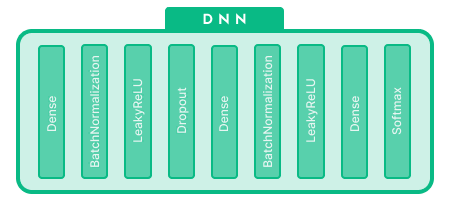
\includegraphics[width=\textwidth]{figures/architecture/DNN.png}
    \caption{Especialista DNN ($\mathcal{E}_{\mathrm{DNN}}$).}
    \label{subfig:arch_dnn}
\end{subfigure}
\hfill
\begin{subfigure}[b]{0.54\textwidth}
    \centering
    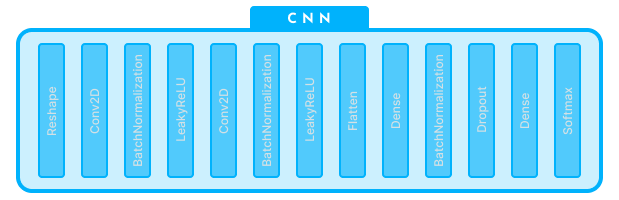
\includegraphics[width=\textwidth]{figures/architecture/CNN.png}
    \caption{Especialista CNN 2D ($\mathcal{E}_{\mathrm{CNN}}$).}
    \label{subfig:arch_cnn}
\end{subfigure}

\vspace{0.3cm}

\begin{subfigure}[b]{0.43\textwidth}
    \centering
    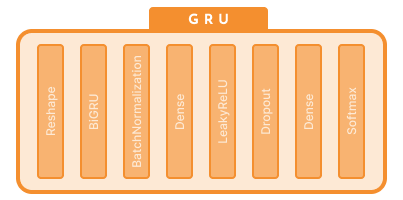
\includegraphics[width=\textwidth]{figures/architecture/GRU.png}
    \caption{Especialista GRU ($\mathcal{E}_{\mathrm{GRU}}$).}
    \label{subfig:arch_gru}
\end{subfigure}
\hfill
\begin{subfigure}[b]{0.53\textwidth}
    \centering
    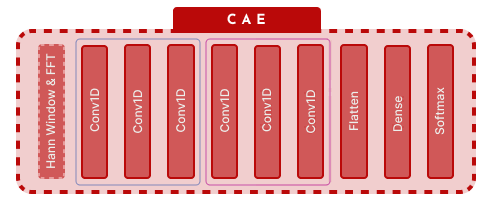
\includegraphics[width=\textwidth]{figures/architecture/CAE.png}
    \caption{Especialista CAE ($\mathcal{E}_{\mathrm{CAE}}$).}
    \label{subfig:arch_cae}
\end{subfigure}

\vspace{0.3cm}

\begin{subfigure}[b]{0.45\textwidth}
    \centering
    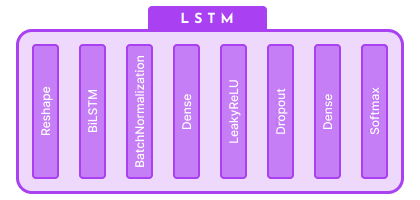
\includegraphics[width=\textwidth]{figures/architecture/LSTM.png}
    \caption{Especialista LSTM ($\mathcal{E}_{\mathrm{LSTM}}$).}
    \label{subfig:arch_lstm}
\end{subfigure}
\fonte{Elaborado pelo autor (2026).}
\end{figure}


\subsection{Gating Network com Refinamento Atencional e Compressão Simétrica}
\label{subsec:gating_network}

A rede de roteamento (\emph{Gating Network}) atua como o árbitro inteligente do comitê de especialistas. Ao contrário de abordagens ensemble com votação estática ou ponderação fixa, a Gating Network inspeciona o vetor completo de telemetria $\mathbf{x} \in \mathbb{R}^{73}$ e calcula dinamicamente a relevância de cada especialista para o fluxo específico sob análise.

Formalmente, a Gating Network processa $\mathbf{x}$ através de duas camadas densas ($128$ e $64$ unidades com Batch Normalization, ativação LeakyReLU com $\alpha=0{,}2$ e Dropout $p=0{,}1$), projetando os logits brutos $\mathbf{z}_{\mathrm{raw}} \in \mathbb{R}^5$, conforme esquematizado na \ref{fig:arch_gating_network}. A distribuição preliminar de confiança $\boldsymbol{\alpha}$ é calculada via Softmax:
\begin{equation}
\label{eq:gating_alpha}
\boldsymbol{\alpha} = \operatorname{softmax}(\mathbf{z}_{\mathrm{raw}}) \in \mathbb{R}^5.
\end{equation}

Em seguida, o vetor $\boldsymbol{\alpha}$ é submetido à camada customizada \texttt{AttentionRefinementLayer}:
\begin{equation}
\label{eq:gating_refinement}
\mathbf{z}_{\mathrm{refined}} = \mathbf{W}_g \ln(\boldsymbol{\alpha} + \epsilon) + \mathbf{b}_g,
\end{equation}
em que $\mathbf{W}_g \in \mathbb{R}^{5 \times 5}$ e $\mathbf{b}_g \in \mathbb{R}^5$ são pesos aprendíveis e $\epsilon = 10^{-7}$ previne instabilidades logarítmicas. Para impedir o colapso e a extinção catastrófica de especialistas (cenário no qual pesos poderiam decair para ordens ínfimas como $10^{-8}$ e desativar especialistas vitais como o CAE), aplica-se a compressão simétrica via tangente hiperbólica:
\begin{equation}
\label{eq:gating_tanh}
\tilde{\mathbf{z}} = \tanh(\mathbf{z}_{\mathrm{refined}}),
\end{equation}
confinando estritamente os logits refinados no intervalo $[-1, 1]$. A distribuição final de pesos atencionais $\mathbf{a}$ é obtida por Softmax temperado:
\begin{equation}
\label{eq:gating_weights}
\mathbf{a} = \operatorname{softmax}\left(\frac{\tilde{\mathbf{z}}}{\tau}\right) = [a_{\mathrm{dnn}}, a_{\mathrm{cnn}}, a_{\mathrm{gru}}, a_{\mathrm{cae}}, a_{\mathrm{lstm}}]^\top,
\end{equation}
em que $\sum_{k=1}^5 a_k = 1$ e $a_k > 0$, mantendo a temperatura inicial calibrada em $\tau = 1{,}0$ \cite{guo2017calibration}.

\begin{figure}[htb]
\centering
\caption{Topologia interna da Gating Network com refinamento atencional e compressão simétrica.}
\label{fig:arch_gating_network}
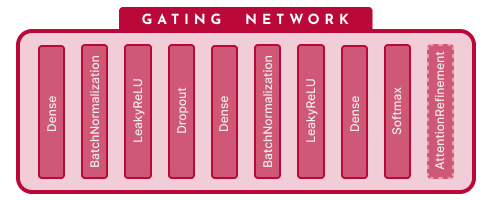
\includegraphics[width=0.75\textwidth]{figures/architecture/GATING_NETWORK.png}
\fonte{Elaborado pelo autor (2026).}
\end{figure}


\subsection{Mecanismo Attention-based Learnable Fusion (ALF)}
\label{subsec:mecanismo_alf}

A integração final das decisões é conduzida pelo módulo customizado \textbf{ALF} (\emph{Attention-based Learnable Fusion}), cuja topologia interna é apresentada na \ref{fig:arch_alf}, estruturado em dois blocos determinísticos:

\begin{enumerate}
    \item \textbf{Fusão Estrita por Soma Ponderada (\texttt{WeightedSumFusion}):}
    A camada de fusão recebe as distribuições probabilísticas preditas por cada um dos cinco especialistas $\{\hat{\mathbf{y}}^{(k)}\}_{k=1}^5 \subset \mathbb{R}^C$ e o vetor de pesos atencionais $\mathbf{a} \in \mathbb{R}^5$ proveniente da Gating Network, efetuando a soma ponderada estrita:
    \begin{equation}
    \label{eq:alf_weighted_sum}
    \mathbf{z} = \sum_{k=1}^5 a_k \cdot \hat{\mathbf{y}}^{(k)} \in \mathbb{R}^C.
    \end{equation}
    Nenhuma conexão residual externa ou concatenação paralela contorna a soma ponderada. Essa decisão de projeto impõe que $100\%$ do fluxo de gradientes retropropagados atravesse a ponderação $a_k \hat{\mathbf{y}}^{(k)}$, forçando a Gating Network a exercer sua função seletiva e incentivando a especialização real de cada rede neural;
    
    \item \textbf{Cabeça Profunda de Decisão Multiclasse:}
    O vetor fundido $\mathbf{z}$ é subsequentemente processado por uma cabeça classificadora profunda desenhada para refinar as margens de decisão entre classes com alta sobreposição:
    \begin{align}
    \label{eq:alf_deep_head_1}
    \mathbf{u}_1 &= \operatorname{LeakyReLU}_{0{,}2}(\operatorname{BN}(\mathbf{W}_1 \mathbf{z} + \mathbf{b}_1)) \in \mathbb{R}^{128}, \\
    \mathbf{u}_1^{\mathrm{drop}} &= \operatorname{Dropout}_{0{,}1}(\mathbf{u}_1), \\
    \mathbf{u}_2 &= \operatorname{LeakyReLU}_{0{,}2}(\operatorname{BN}(\mathbf{W}_2 \mathbf{u}_1^{\mathrm{drop}} + \mathbf{b}_2)) \in \mathbb{R}^{64}, \\
    \label{eq:saida_alf_softmax}
    \hat{\mathbf{y}}_{\mathrm{ALF}} &= \operatorname{softmax}(\mathbf{W}_3 \mathbf{u}_2 + \mathbf{b}_3) \in \mathbb{R}^C.
    \end{align}
\end{enumerate}

\begin{figure}[htb]
\centering
\caption{Topologia interna do módulo de fusão ALF (\emph{Attention-based Learnable Fusion}).}
\label{fig:arch_alf}
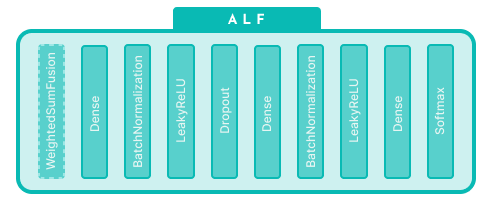
\includegraphics[width=0.75\textwidth]{figures/architecture/ALF.png}
\fonte{Elaborado pelo autor (2026).}
\end{figure}

A arquitetura macroscópica unificada do modelo ALF-MoE, integrando a recepção da telemetria de rede, o roteamento pelos especialistas heterogêneos, a arbitragem dinâmica pela Gating Network e a combinação ponderada das probabilidades com refinamento profundo no módulo ALF, é ilustrada na \ref{fig:arch_alf_moe}.

\begin{figure}[htb]
\centering
\caption{Visão arquitetural integrada do modelo ALF-MoE, evidenciando o fluxo de tensores entre especialistas, Gating Network e fusão ALF.}
\label{fig:arch_alf_moe}
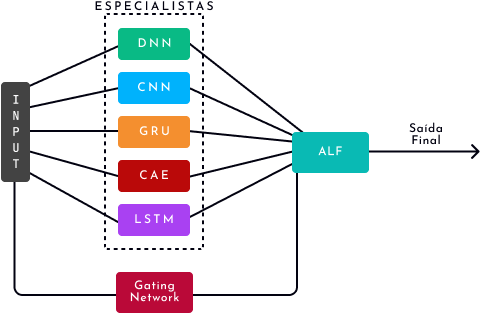
\includegraphics[width=0.75\textwidth]{figures/architecture/ALF-MoE.png}
\fonte{Elaborado pelo autor (2026).}
\end{figure}


\section{Protocolo Experimental de Treinamento e Avaliação}
\label{sec:protocolo_experimental}

Para garantir rigor metodológico e reprodutibilidade, todos os ensaios foram balizados por um protocolo padronizado de otimização multitarefa, particionamento e validação estatística.

\subsection{Funções de Perda e Otimização Multitarefa}
\label{subsec:funcoes_perda}

O treinamento do modelo ALF-MoE é formulado como uma otimização multitarefa conjunta (\emph{multi-task learning}). A função de custo global $\mathcal{L}_{\mathrm{total}}$ agrega a perda da cabeça principal de fusão ALF, as perdas supervisionadas auxiliares dos cinco especialistas e a perda mista de reconstrução espectral do Autoencoder Convolucional:
\begin{equation}
\label{eq:perda_multitarefa}
\mathcal{L}_{\mathrm{total}} = 1{,}0 \cdot \mathcal{L}_{\mathrm{FL}}(\hat{\mathbf{y}}_{\mathrm{ALF}}, \mathbf{y}) + 0{,}2 \sum_{k=1}^5 \mathcal{L}_{\mathrm{FL}}(\hat{\mathbf{y}}^{(k)}, \mathbf{y}) + \lambda_{\mathrm{rec}} \mathcal{L}_{\mathrm{CAE,rec}},
\end{equation}
sendo $\lambda_{\mathrm{rec}} = 1{,}0$ e o peso das cabeças auxiliares fixado em $0{,}2$, provendo sinal de gradiente para guiar os especialistas sem sobrecarregar a convergência da cabeça unificada ALF.

A perda de classificação empregada em todas as cabeças é a \textbf{Focal Loss Multiclasse} \cite{lin2017focal}, definida por:
\begin{equation}
\label{eq:focal_loss}
\mathcal{L}_{\mathrm{FL}}(p_t) = -\alpha_t (1 - p_t)^\gamma \ln(p_t),
\end{equation}
em que $p_t$ representa a probabilidade estimada pelo modelo para a classe verdadeira, $\gamma = 2{,}0$ atua como o parâmetro de foco que suprime gradientes de exemplos fáceis e bem classificados, e $\alpha_t = w_c$ corresponde aos pesos balanceados por raiz quadrada definidos na Equação~\ref{eq:class_weights}.

O otimizador utilizado é o \textbf{Adam} com taxa de aprendizado inicial $\eta_0 = 10^{-3}$, momentos $\beta_1 = 0{,}9$, $\beta_2 = 0{,}999$, $\epsilon = 10^{-8}$ e tamanho de lote (\emph{batch size}) fixado em $128$ instâncias ao longo de $10$ épocas. O agendamento da taxa de aprendizado é governado pelo mecanismo \texttt{ReduceLROnPlateau} (fator de redução $0{,}5$, paciência de $2$ épocas monitorando \texttt{val\_ALF\_F1-Score} com limiar inferior de $10^{-6}$), complementado por parada precoce (\texttt{EarlyStopping}) com paciência de $4$ épocas monitorando a mesma métrica.


\subsection{Métricas de Avaliação}
\label{subsec:metricas_avaliacao}

A avaliação de desempenho do modelo e de cada especialista individual engloba métricas de eficácia preditiva e métricas de eficiência computacional em tempo de execução.

\subsubsection{Métricas de Eficácia Estatística}

Para cada classe $c \in \{0, \dots, C-1\}$, denotam-se $TP_c, FP_c, FN_c, TN_c$ os quantitativos de verdadeiros positivos, falsos positivos, falsos negativos e verdadeiros negativos, respectivamente. Computam-se:
\begin{enumerate}
    \item \textbf{Acurácia Global ($\mathrm{Acc}$):}
    \begin{equation}
    \mathrm{Acc} = \frac{\sum_{c=0}^{C-1} TP_c}{\sum_{c=0}^{C-1} (TP_c + FN_c)};
    \end{equation}
    
    \item \textbf{Acurácia Balanceada ($\mathrm{Acc}_{\mathrm{bal}}$):} média aritmética das taxas de recall sobre todas as classes, mitigando a distorção induzida por classes majoritárias:
    \begin{equation}
    \mathrm{Acc}_{\mathrm{bal}} = \frac{1}{C} \sum_{c=0}^{C-1} \frac{TP_c}{TP_c + FN_c};
    \end{equation}
    
    \item \textbf{Precisão Macro ($\mathrm{Prec}_{\mathrm{macro}}$) e Sensibilidade Macro ($\mathrm{Rec}_{\mathrm{macro}}$):}
    \begin{equation}
    \mathrm{Prec}_{\mathrm{macro}} = \frac{1}{C} \sum_{c=0}^{C-1} \frac{TP_c}{TP_c + FP_c}, \quad \mathrm{Rec}_{\mathrm{macro}} = \frac{1}{C} \sum_{c=0}^{C-1} \frac{TP_c}{TP_c + FN_c};
    \end{equation}
    
    \item \textbf{Macro $F_1$-Score ($F_1^{\mathrm{macro}}$):} média harmônica entre precisão e sensibilidade computada de forma não ponderada, constituindo o critério primordial para ranqueamento de NIDS sob desbalanceamento:
    \begin{equation}
    F_1^{\mathrm{macro}} = \frac{1}{C} \sum_{c=0}^{C-1} \frac{2 \cdot \mathrm{Prec}_c \cdot \mathrm{Rec}_c}{\mathrm{Prec}_c + \mathrm{Rec}_c};
    \end{equation}
    
    \item \textbf{Weighted $F_1$-Score ($F_1^{\mathrm{weighted}}$):} ponderação das pontuações $F_1$ pela proporção empírica de amostras de cada classe $N_c / N$.
\end{enumerate}

\subsubsection{Métricas de Eficiência Computacional}

A viabilidade de implantação do NIDS em nós de monitoramento em tempo real depende estritamente do tempo de processamento. Avaliam-se:
\begin{enumerate}
    \item \textbf{Latência por Amostra ($L_{\mathrm{sample}}$):} tempo médio transcorrido para inferir um único fluxo de rede, expresso em milissegundos por fluxo ($\mathrm{ms/fluxo}$):
    \begin{equation}
    L_{\mathrm{sample}} = \frac{T_{\mathrm{total,inf}}}{N_{\mathrm{test}}} \times 10^3;
    \end{equation}
    
    \item \textbf{Vazão de Inferência ($\mathrm{Throughput}$):} taxa de processamento sustentada expressa em fluxos por segundo ($\mathrm{fluxos/s}$):
    \begin{equation}
    \mathrm{Throughput} = \frac{N_{\mathrm{test}}}{T_{\mathrm{total,inf}}}.
    \end{equation}
\end{enumerate}


%------------------------------------------------------------------------------------%
\chapter{Pipeline de Extração e Ambiente de Inferência}
\label{cap:pipeline}
\section{Captura e Processamento de Tráfego}
\label{sec:captura_processamento}
% [Seção reservada - aguardando conclusão dos testes pelo autor]

\subsection{Extração com NFStream}
\label{subsec:extracao_nfstream}
% [Seção reservada - aguardando conclusão dos testes pelo autor]

\subsection{Mapeamento e Alinhamento de Features (NFStream \texorpdfstring{$\to$}{->} CICFlowMeter)}
\label{subsec:mapeamento_features}
% [Seção reservada - aguardando conclusão dos testes pelo autor]

\section{Setup de Inferência em Tempo Real}
\label{sec:setup_inferencia}
% [Seção reservada - aguardando conclusão dos testes pelo autor]

\subsection{Arquitetura do Ambiente de Execução}
\label{subsec:arquitetura_execucao}
% [Seção reservada - aguardando conclusão dos testes pelo autor]

\subsection{Cenários de Teste de Estresse (Benigno, Ataques Humanos e Agentes via LLM)}
\label{subsec:cenarios_estresse}
% [Seção reservada - aguardando conclusão dos testes pelo autor]


%------------------------------------------------------------------------------------%
\chapter{Resultados e Discussão}
\label{cap:resultados}
\section{Desempenho nos Datasets de Benchmark (Resultados Offline)}
\label{sec:desempenho_benchmark}

A validação empírica da arquitetura **ALF-MoE** foi conduzida sob um protocolo rigoroso de teste em partições estritamente desacopladas (\emph{offline test sets}), cobrindo os quatro conjuntos de dados analisados em sete configurações experimentais independentes. Este protocolo permitiu avaliar: (i) a capacidade de discriminação sob diferentes níveis de abstração semântica (\emph{Threat Levels} 0 e 2); (ii) a resiliência do modelo diante de falhas de rotulação em dados legados e o ganho obtido após a sanitização SOTA de \citeonline{liu2022error}; e (iii) a contribuição individual de cada especialista neural versus a representação integrada alcançada pelo bloco atencional ALF.


\subsection{Análise por Classe e Desempenho Global}
\label{subsec:analise_classe_global}

A Tabela~\ref{tab:desempenho_global_7cenarios} consolida os resultados quantitativos globais do modelo ALF-MoE em todas as matrizes experimentais avaliadas. As métricas reportadas englobam Acurácia Global ($\mathrm{Acc}$), Macro $F_1$-Score ($F_1^{\mathrm{macro}}$), Macro Precisão ($\mathrm{Prec}_{\mathrm{macro}}$), Macro Sensibilidade ($\mathrm{Rec}_{\mathrm{macro}}$), Latência por Amostra ($L_{\mathrm{sample}}$) e Vazão de Inferência ($\mathrm{Throughput}$).

\begin{table}[htb]
\centering
\caption{Desempenho global consolidado do modelo ALF-MoE nos 7 cenários de benchmark.}
\label{tab:desempenho_global_7cenarios}
\footnotesize
\setlength{\tabcolsep}{3.5pt}
\begin{tabularx}{\textwidth}{>{\raggedright\arraybackslash}X l rrrrrr}
\hline
\textbf{Conjunto de Dados} & \textbf{Cenário} & \textbf{Acurácia} & \textbf{Macro $F_1$} & \textbf{Precisão} & \textbf{Recall} & \textbf{Latência} & \textbf{Vazão} \\
\hline
CIC-UNSW-NB15 & L0 (10 cls) & 75,11\% & 0,5069 & 0,5103 & 0,6087 & 0,0479\,ms & 20.896\,fl/s \\
CIC-BCCC-NRC-2024 & L0 (49 cls) & 82,29\% & 0,4501 & 0,4505 & 0,5095 & 0,0184\,ms & 54.258\,fl/s \\
CIC-BCCC-NRC-2024 & L2 (9 cls) & 92,83\% & 0,8476 & 0,8382 & 0,8617 & 0,0122\,ms & 82.129\,fl/s \\
CSE-CIC-IDS2018 (Orig.) & L0 (15 cls) & 98,96\% & 0,8773 & 0,9045 & 0,8669 & 0,0119\,ms & 84.135\,fl/s \\
CSE-CIC-IDS2018 (Orig.) & L2 (7 cls) & 98,38\% & 0,9050 & 0,9658 & 0,8855 & 0,0111\,ms & 90.017\,fl/s \\
CSE-CIC-IDS2018 (Corr.) & L0 (15 cls) & 99,97\% & 0,8918 & 0,8814 & 0,9144 & 0,0162\,ms & 61.765\,fl/s \\
CSE-CIC-IDS2018 (Corr.) & L2 (9 cls) & 99,96\% & 0,8851 & 0,9579 & 0,8927 & 0,0118\,ms & 84.858\,fl/s \\
\hline
\end{tabularx}
\fonte{Elaborado pelo autor (2026), a partir dos relatórios experimentais.}
\end{table}

A análise comparativa dos resultados experimentais desdobra-se em três eixos centrais de discussão:

\subsubsection{Eixo 1: Impacto da Granularidade de Ameaças (Nível 0 vs. Nível 2)}

A transição entre o Nível de Ameaça 0 (classes brutas com assinaturas estritas) e o Nível de Ameaça 2 (meta-categorias operacionais consolidadas) evidencia o custo estatístico da discriminação em espaços de classes hiper-fragmentados:
\begin{itemize}
    \item No ambiente IoT (\textbf{CIC-BCCC-NRC-2024}), a consolidação de 49 classes granulares em 9 macro-famílias proporcionou uma elevação substantiva no Macro $F_1$-Score, saltando de $0{,}4501$ para $0{,}8476$ (um incremento relativo de $+88{,}3\%$), acompanhado pelo aumento da Acurácia Global de $82{,}29\%$ para $92{,}83\%$. No nível granular (L0), o modelo é compelido a distinguir entre 12 variantes microscópicas de varredura e múltiplas ramificações de inundações ICMP/UDP cuja separabilidade estatística no nível de fluxo agregado é tênue, muitas com suporte inferior a 200 instâncias de teste. Ao agregar essas variantes em famílias funcionais (como \emph{Reconnaissance}, \emph{DDoS} e \emph{IoT/MQTT}), a incerteza intra-classe é eliminada, gerando um modelo de altíssima confiabilidade operacional para acionamento perimetral;
    \item Em termos de eficiência computacional, a redução do espaço de saída no CIC-BCCC-NRC-2024 aliviou a carga de computação da projeção linear final, reduzindo a latência de $0{,}0184\,\mathrm{ms}$ para $0{,}0122\,\mathrm{ms}$ por fluxo e elevando a vazão sustentada de $54.258$ para $82.129\,\mathrm{fluxos/s}$.
\end{itemize}

\subsubsection{Eixo 2: Impacto da Sanitização de Rótulos de Liu et al. (2022) no CSE-CIC-IDS2018}

O contraste direto entre o CSE-CIC-IDS2018 Canônico e a versão corrigida segundo \citeonline{liu2022error} elucida de forma categórica as consequências do ruído de rotulação em modelos de aprendizado profundo:
\begin{itemize}
    \item Na versão original canônica (L0), o modelo atinge $98{,}96\%$ de acurácia global com Macro $F_1$ de $0{,}8773$. Contudo, a inspeção detalhada por classe revela anomalias críticas: a classe \emph{FTP-BruteForce} obteve $F_1$ de $0{,}7344$ e precisão de apenas $0{,}6843$. Essa degradação decorre diretamente da falha de etiquetagem comprovada por \citeonline{liu2022error}, na qual o servidor na porta 21 estava inativo e respondia com pacotes de encerramento \texttt{[RST, ACK]}. O classificador era forçado a aprender que respostas legítimas de porta fechada equivaliam a força bruta ativa, gerando confusão sistemática com o tráfego normal;
    \item Na versão corrigida (\emph{CSE-CIC-IDS2018 Improved}), na qual fluxos com portas fechadas e tentativas inócuas foram reclassificados como benignos, a Acurácia Global alcançou expressivos $99{,}97\%$ e o Weighted $F_1$-Score atingiu $0{,}9997$ no teste independente de 1.263.903 fluxos;
    \item Além disso, a desagregação da infiltração em classes específicas permitiu constatar que o modelo detecta varreduras internas (\emph{Infiltration - NMAP Portscan}) com $F_1 = 0{,}9912$ e canais de comando vítima-atacante com $F_1 = 0{,}8636$. Em contrapartida, a exfiltração pontual em tráfego criptografado (\emph{Infiltration - Dropbox Download}), representada por meras 17 amostras de teste, obteve $F_1 = 0{,}1818$, demonstrando que conexões legítimas a serviços de nuvem HTTPS constituem o vetor de maior furtividade para extratores baseados puramente em estatísticas de fluxo sem inspeção de carga útil.
\end{itemize}

\subsubsection{Eixo 3: Generalização em Tráfego de Alta Densidade (CIC-UNSW-NB15)}

No conjunto CIC-UNSW-NB15, que não sofreu agregação em níveis superiores (operando estritamente em L0 com 10 classes), o ALF-MoE alcançou Acurácia Global de $75{,}11\%$ e Macro $F_1$-Score de $0{,}5069$. Em classes de tráfego volumétrico e ataques de penetração complexos, o modelo exibiu excelente discriminação: \emph{Benign} ($F_1 = 0{,}9495$), \emph{Fuzzers} ($F_1 = 0{,}6968$), \emph{Exploits} ($F_1 = 0{,}6876$) e \emph{Reconnaissance} ($F_1 = 0{,}7169$). 

Para categorias com suporte diminuto, a função de perda Focal Loss balanceada priorizou a sensibilidade em detrimento da precisão: na classe \emph{Analysis} (suporte 77), o modelo obteve Sensibilidade (\emph{Recall}) de $0{,}9481$ (Acurácia Balanceada de $0{,}9661$), prevenindo a omissão do ataque embora gerando falsos positivos que reduziram o $F_1$ para $0{,}2479$. Esse comportamento reflete a postura conservadora deliberadamente imposta pelo fator de foco da Focal Loss, indispensável para ambientes corporativos em que o custo de um falso negativo (uma invasão ignorada) é infinitamente superior ao de uma inspeção secundária de falso positivo.

\subsubsection{Matrizes de Confusão Normalizadas}

A Figura~\ref{fig:matrizes_confusao_painel} reúne as matrizes de confusão normalizadas para os quatro conjuntos de dados representativos: (a) CSE-CIC-IDS2018 Canônico (L2); (b) CSE-CIC-IDS2018 Corrigido (L2); (c) CIC-BCCC-NRC-2024 (L2); e (d) CIC-UNSW-NB15 (L0).

\begin{figure}[htb]
\centering
\caption{Painel comparativo de matrizes de confusão normalizadas nos quatro cenários de avaliação.}
\label{fig:matrizes_confusao_painel}
\begin{subfigure}[b]{0.48\textwidth}
    \centering
    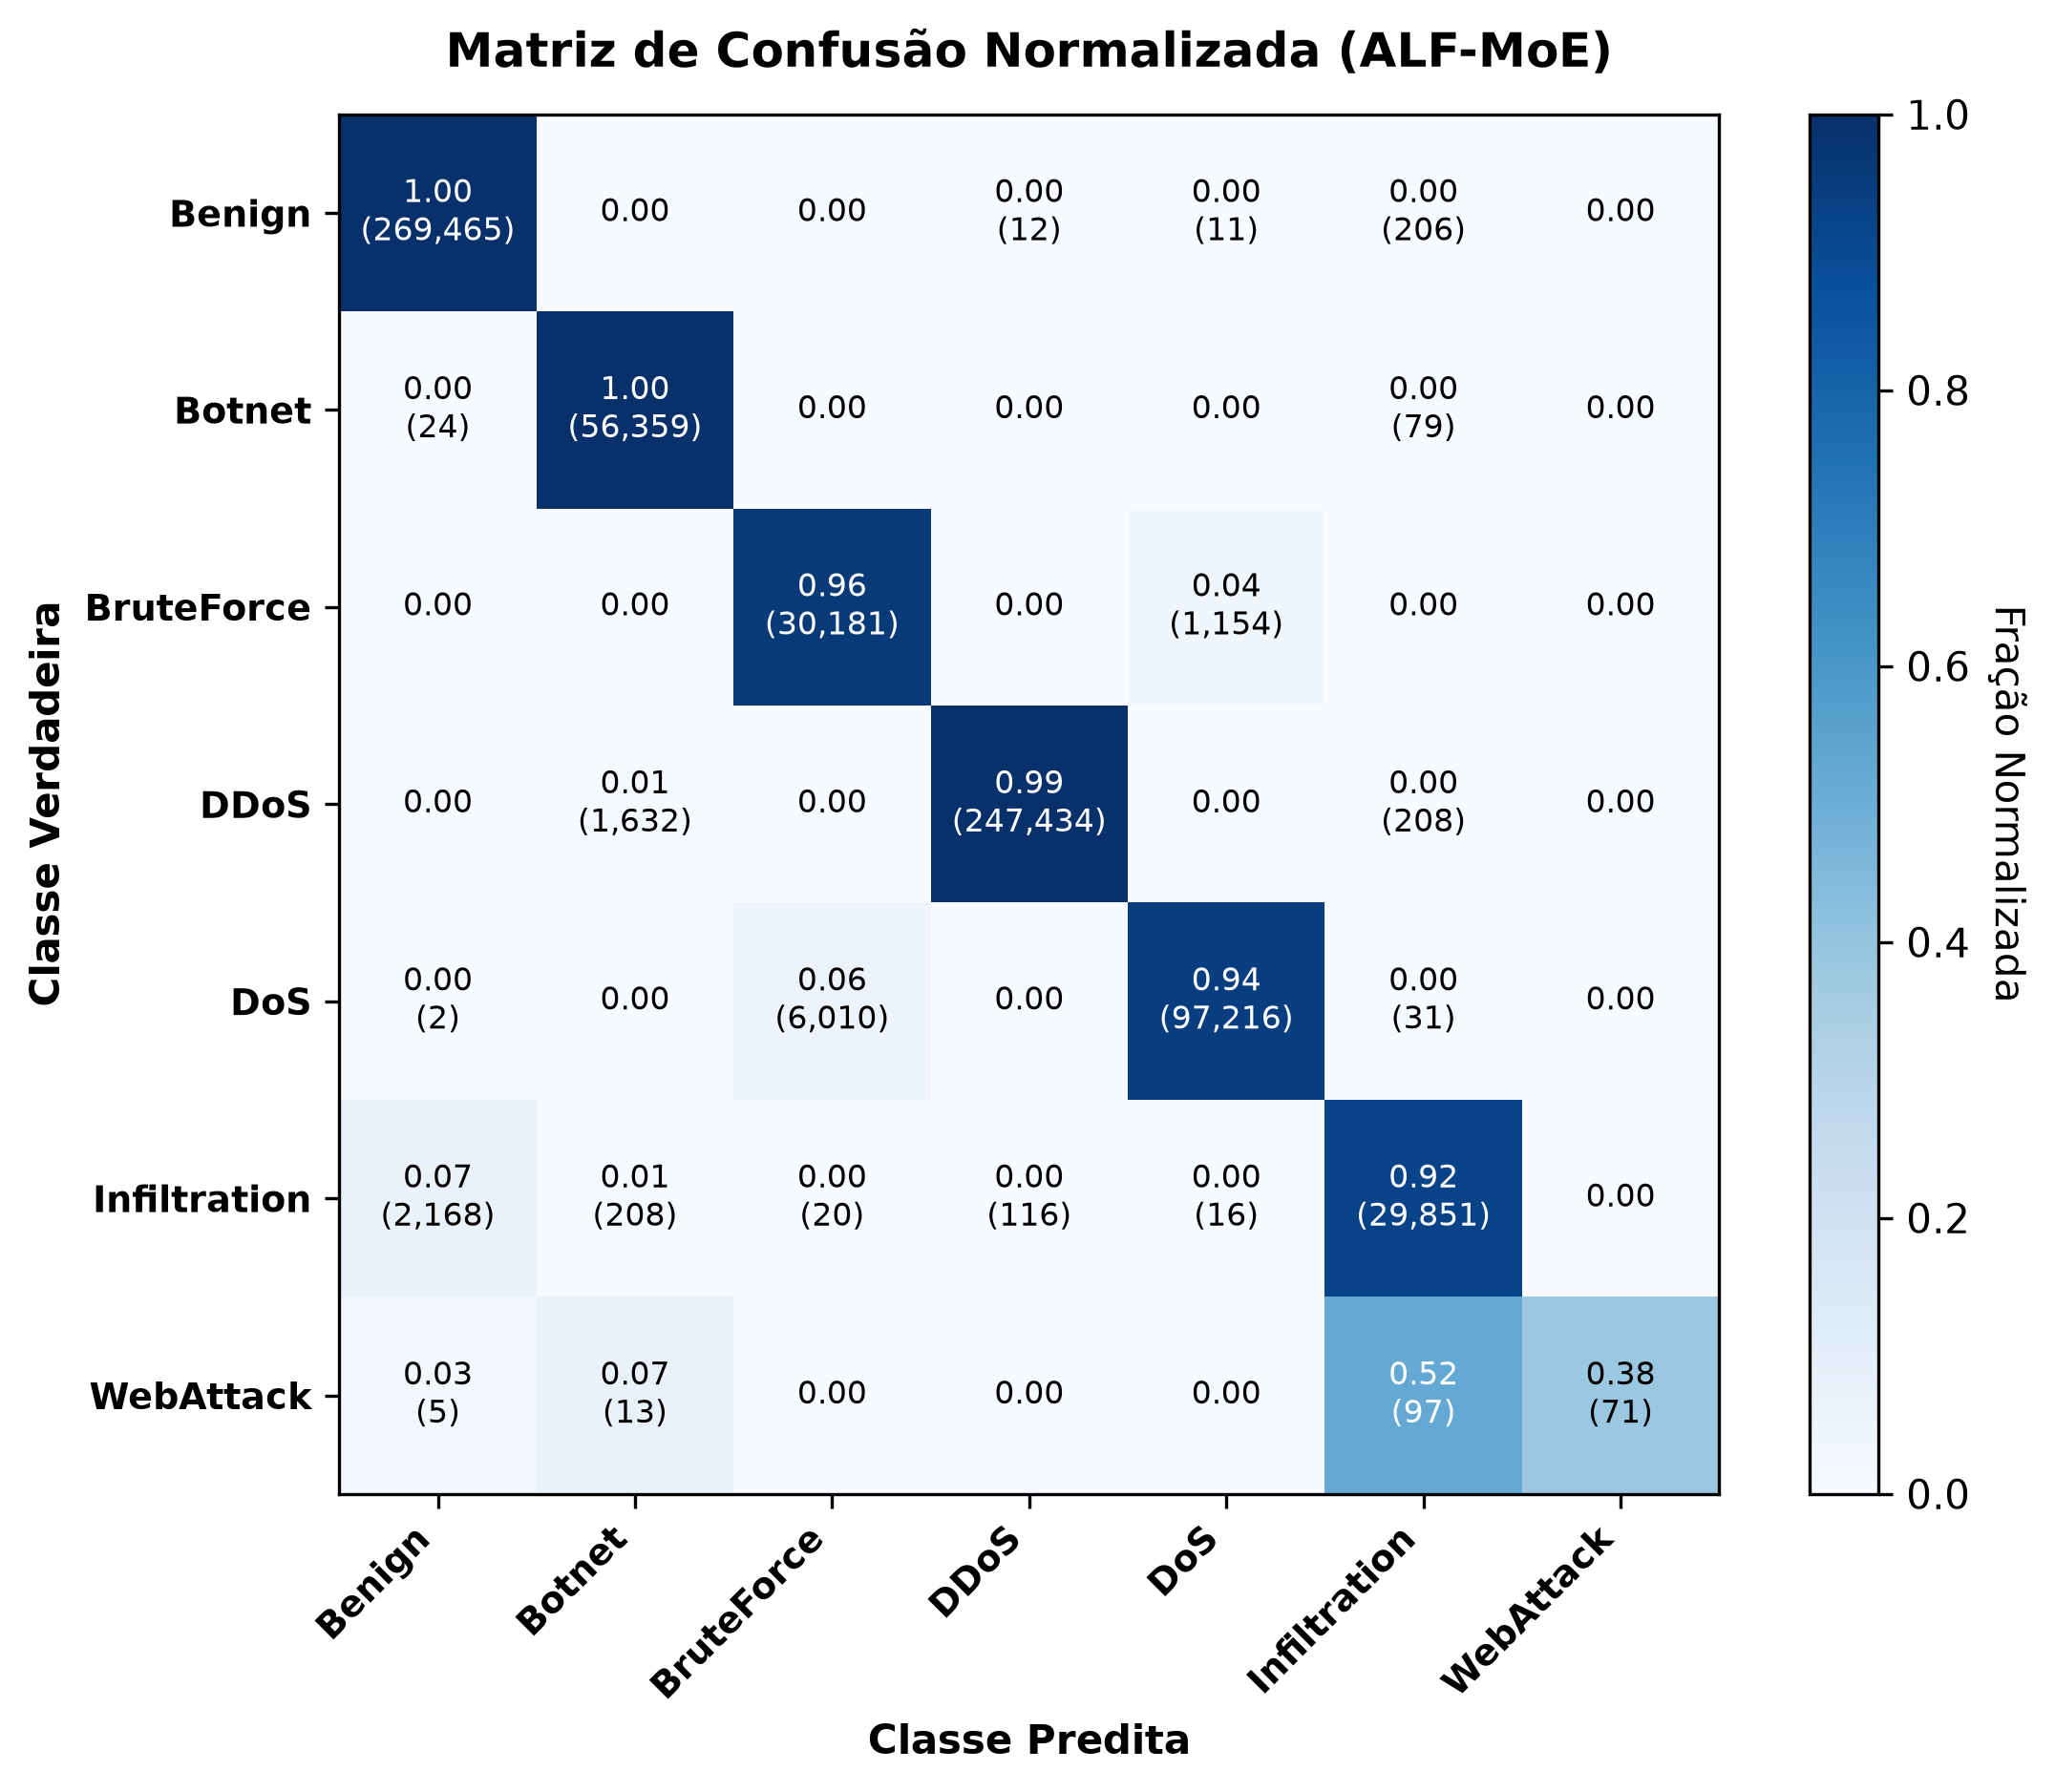
\includegraphics[width=\textwidth]{figures/benchmarks/cm_norm_cse2018_l2.png}
    \caption{CSE-CIC-IDS2018 Canônico (L2 - 7 classes).}
    \label{subfig:cm_cse2018_orig}
\end{subfigure}
\hfill
\begin{subfigure}[b]{0.48\textwidth}
    \centering
    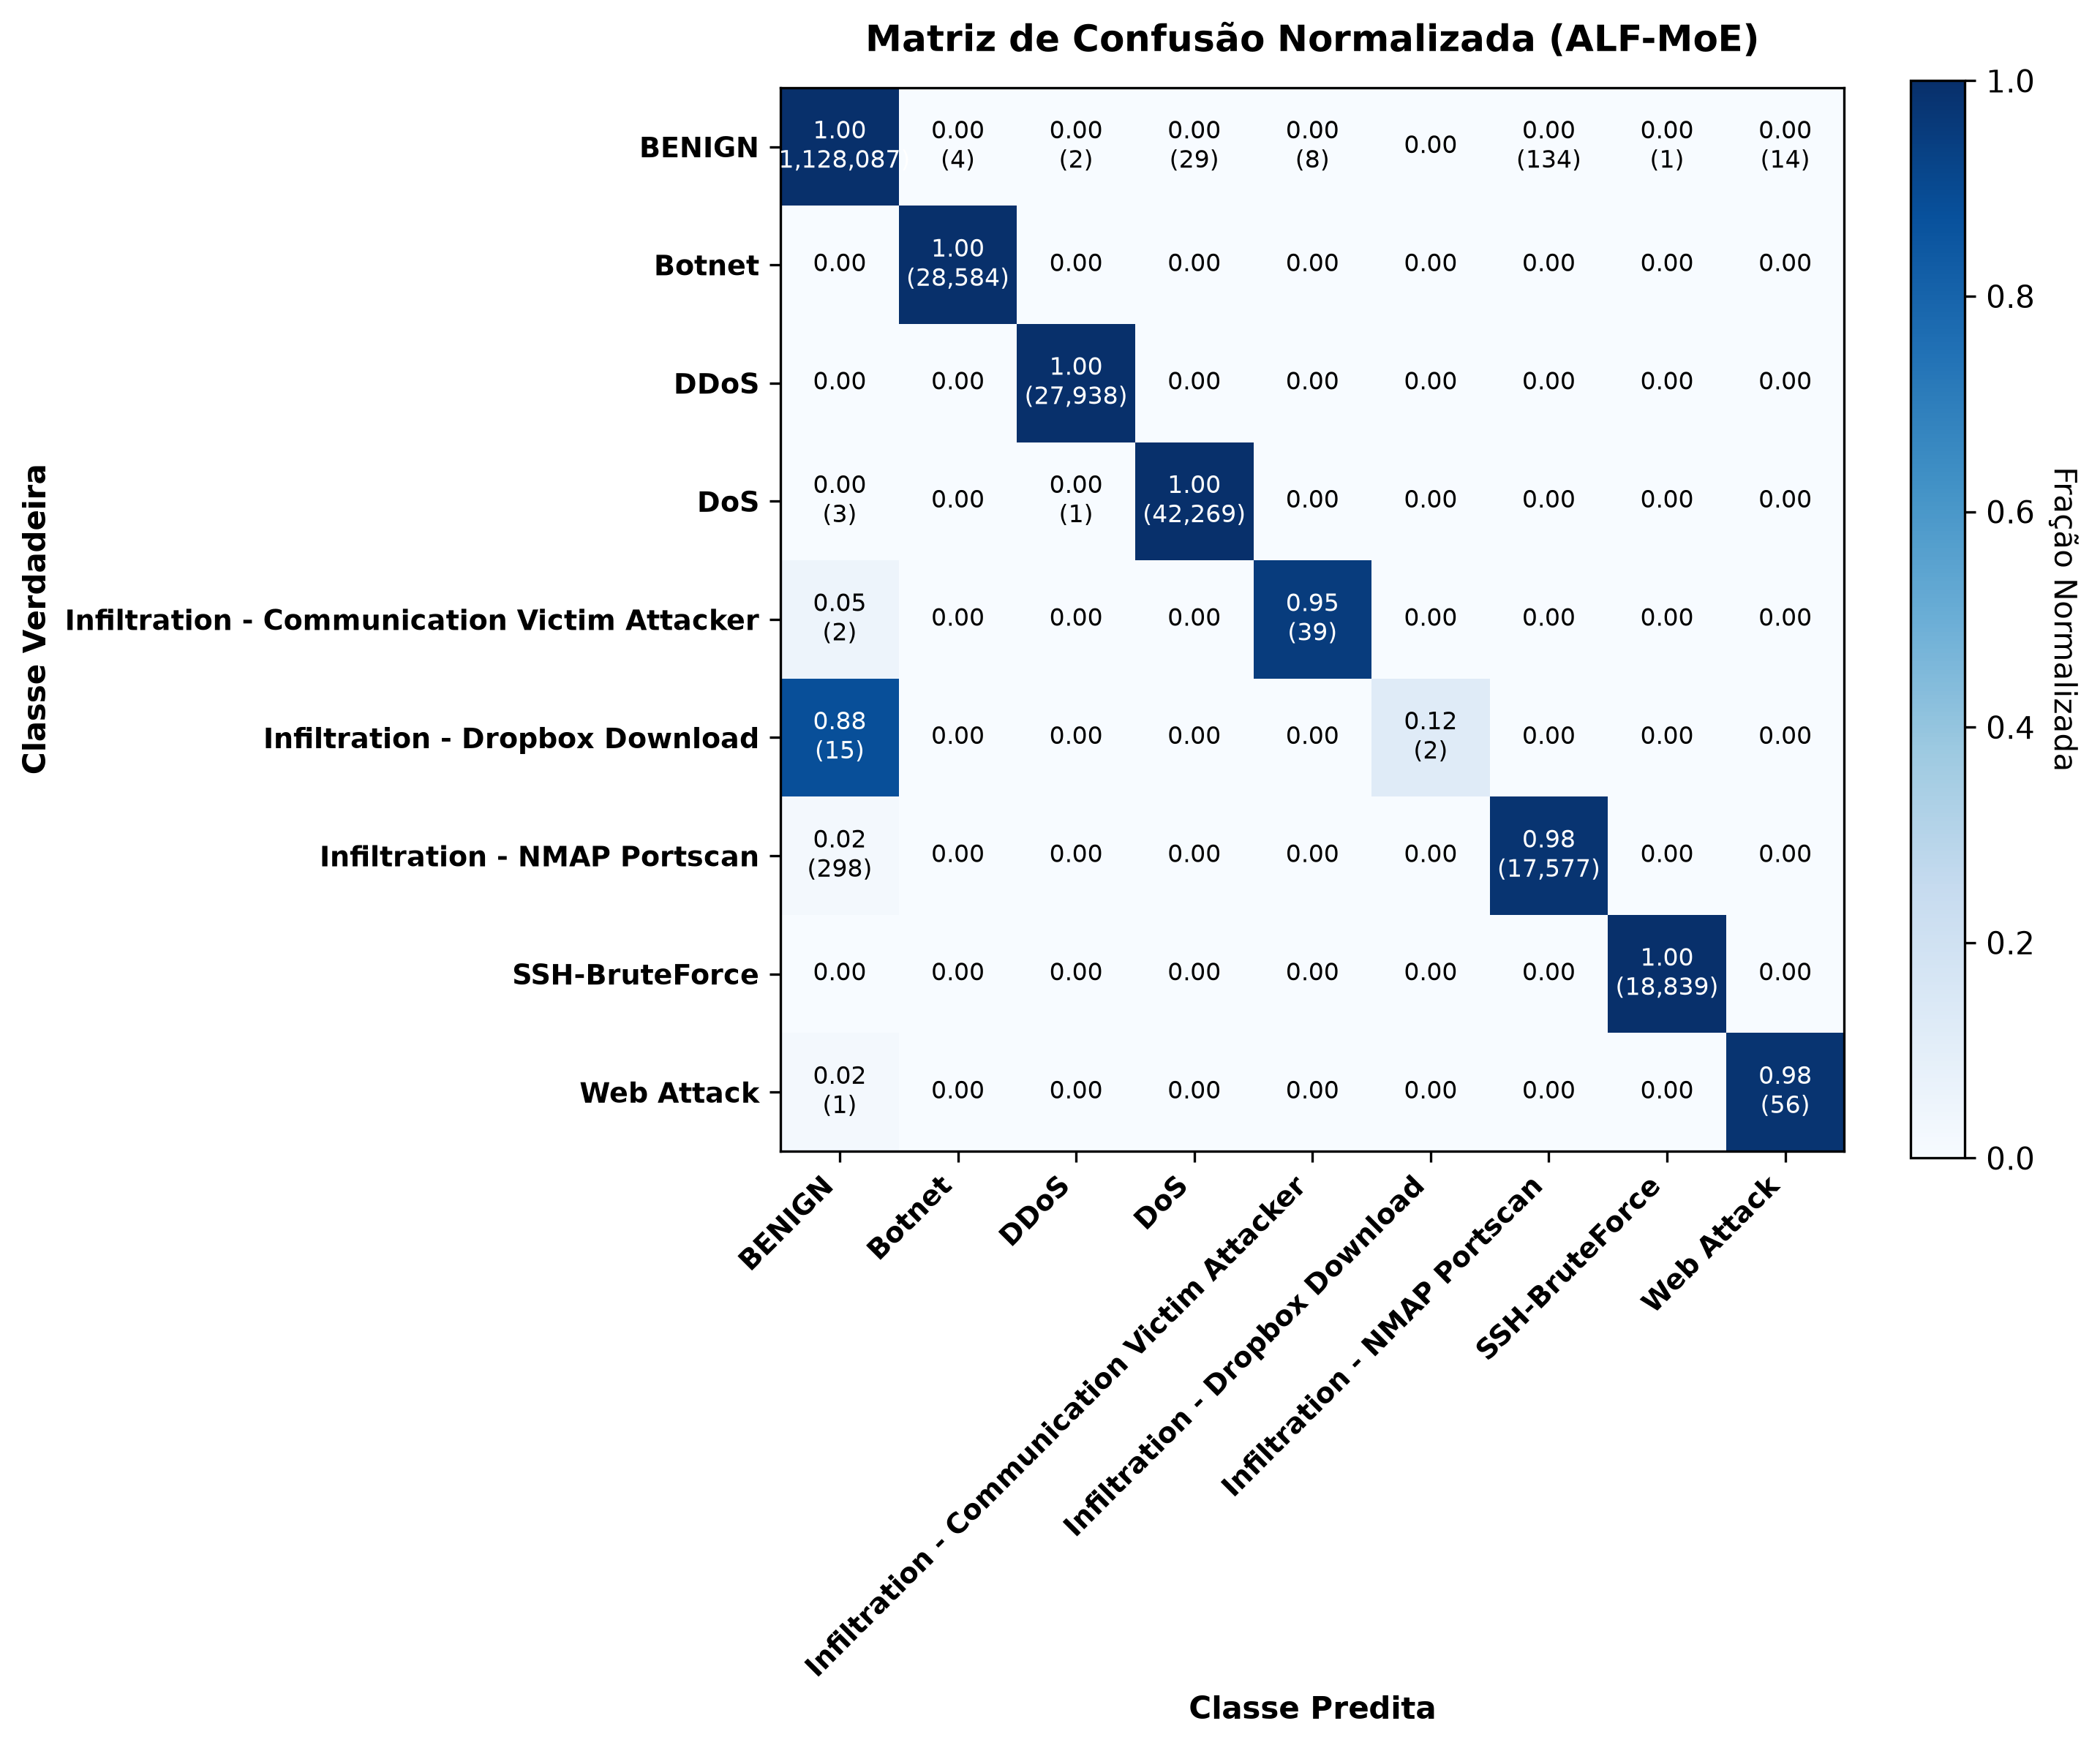
\includegraphics[width=\textwidth]{figures/benchmarks/cm_norm_cse2018_imp_l2.png}
    \caption{CSE-CIC-IDS2018 Corrigido (L2 - 9 classes).}
    \label{subfig:cm_cse2018_imp}
\end{subfigure}

\vspace{0.4cm}

\begin{subfigure}[b]{0.48\textwidth}
    \centering
    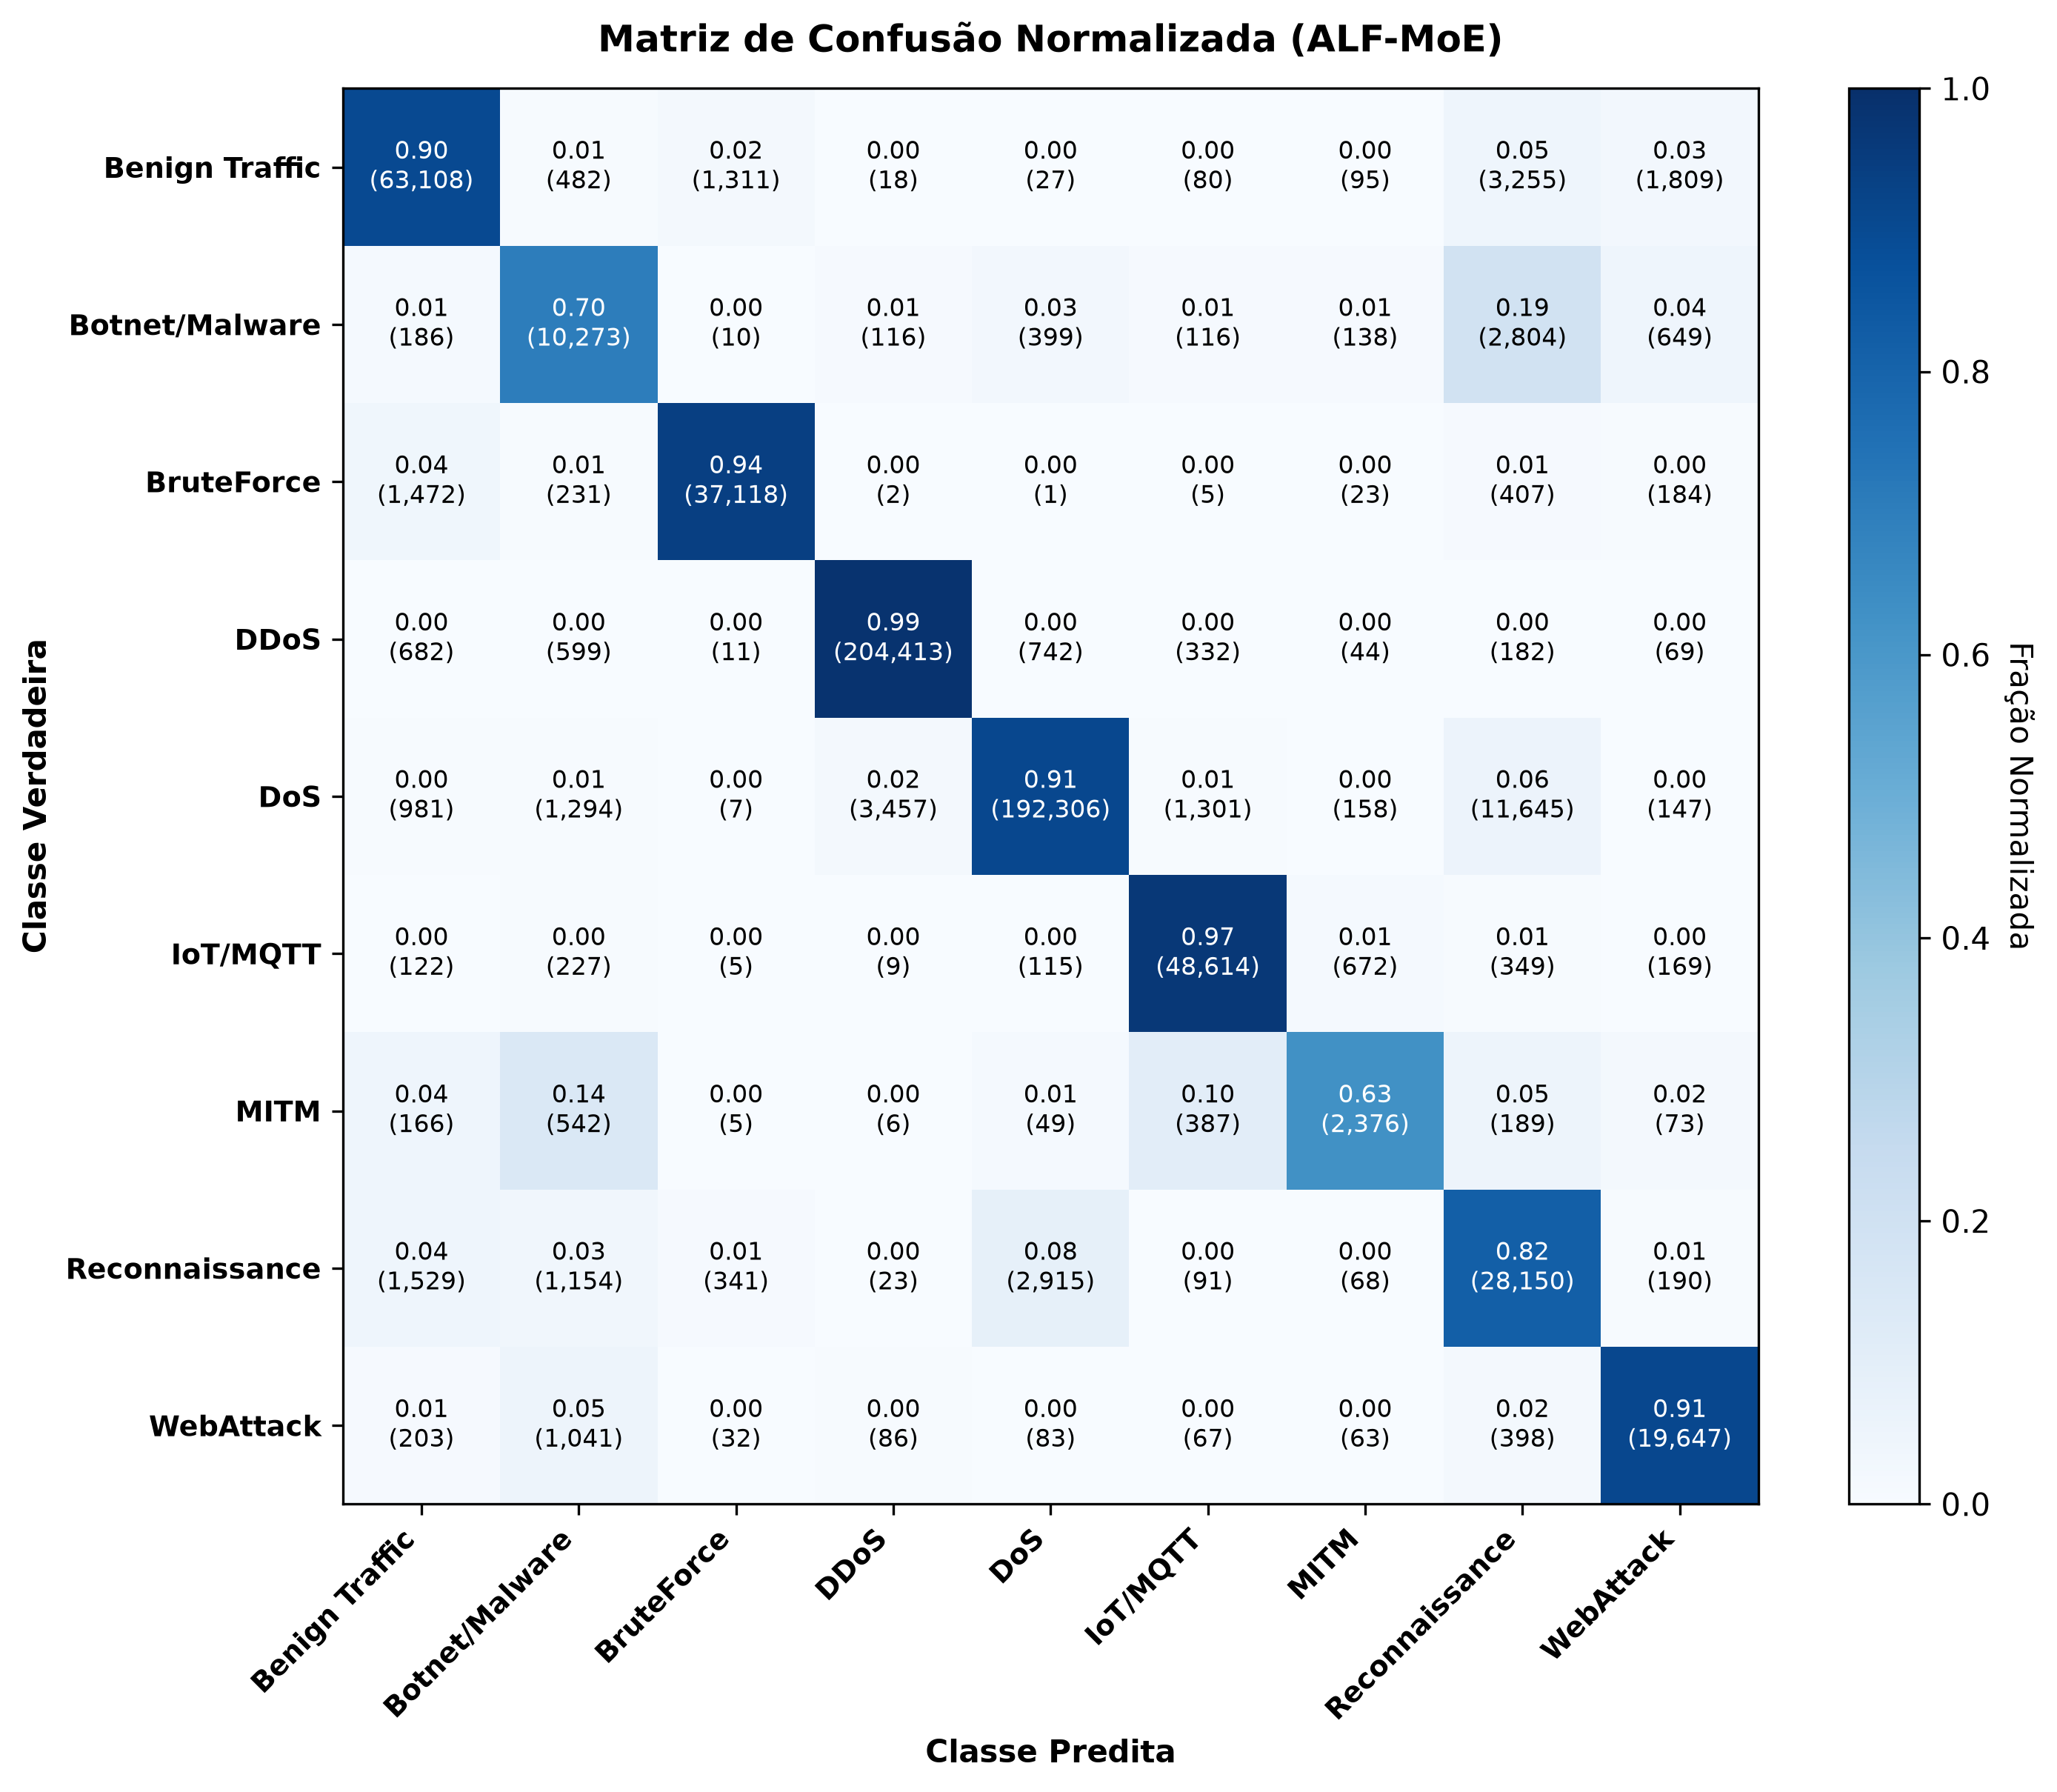
\includegraphics[width=\textwidth]{figures/benchmarks/cm_norm_bccc2024_l2.png}
    \caption{CIC-BCCC-NRC-2024 (L2 - 9 classes).}
    \label{subfig:cm_bccc2024}
\end{subfigure}
\hfill
\begin{subfigure}[b]{0.48\textwidth}
    \centering
    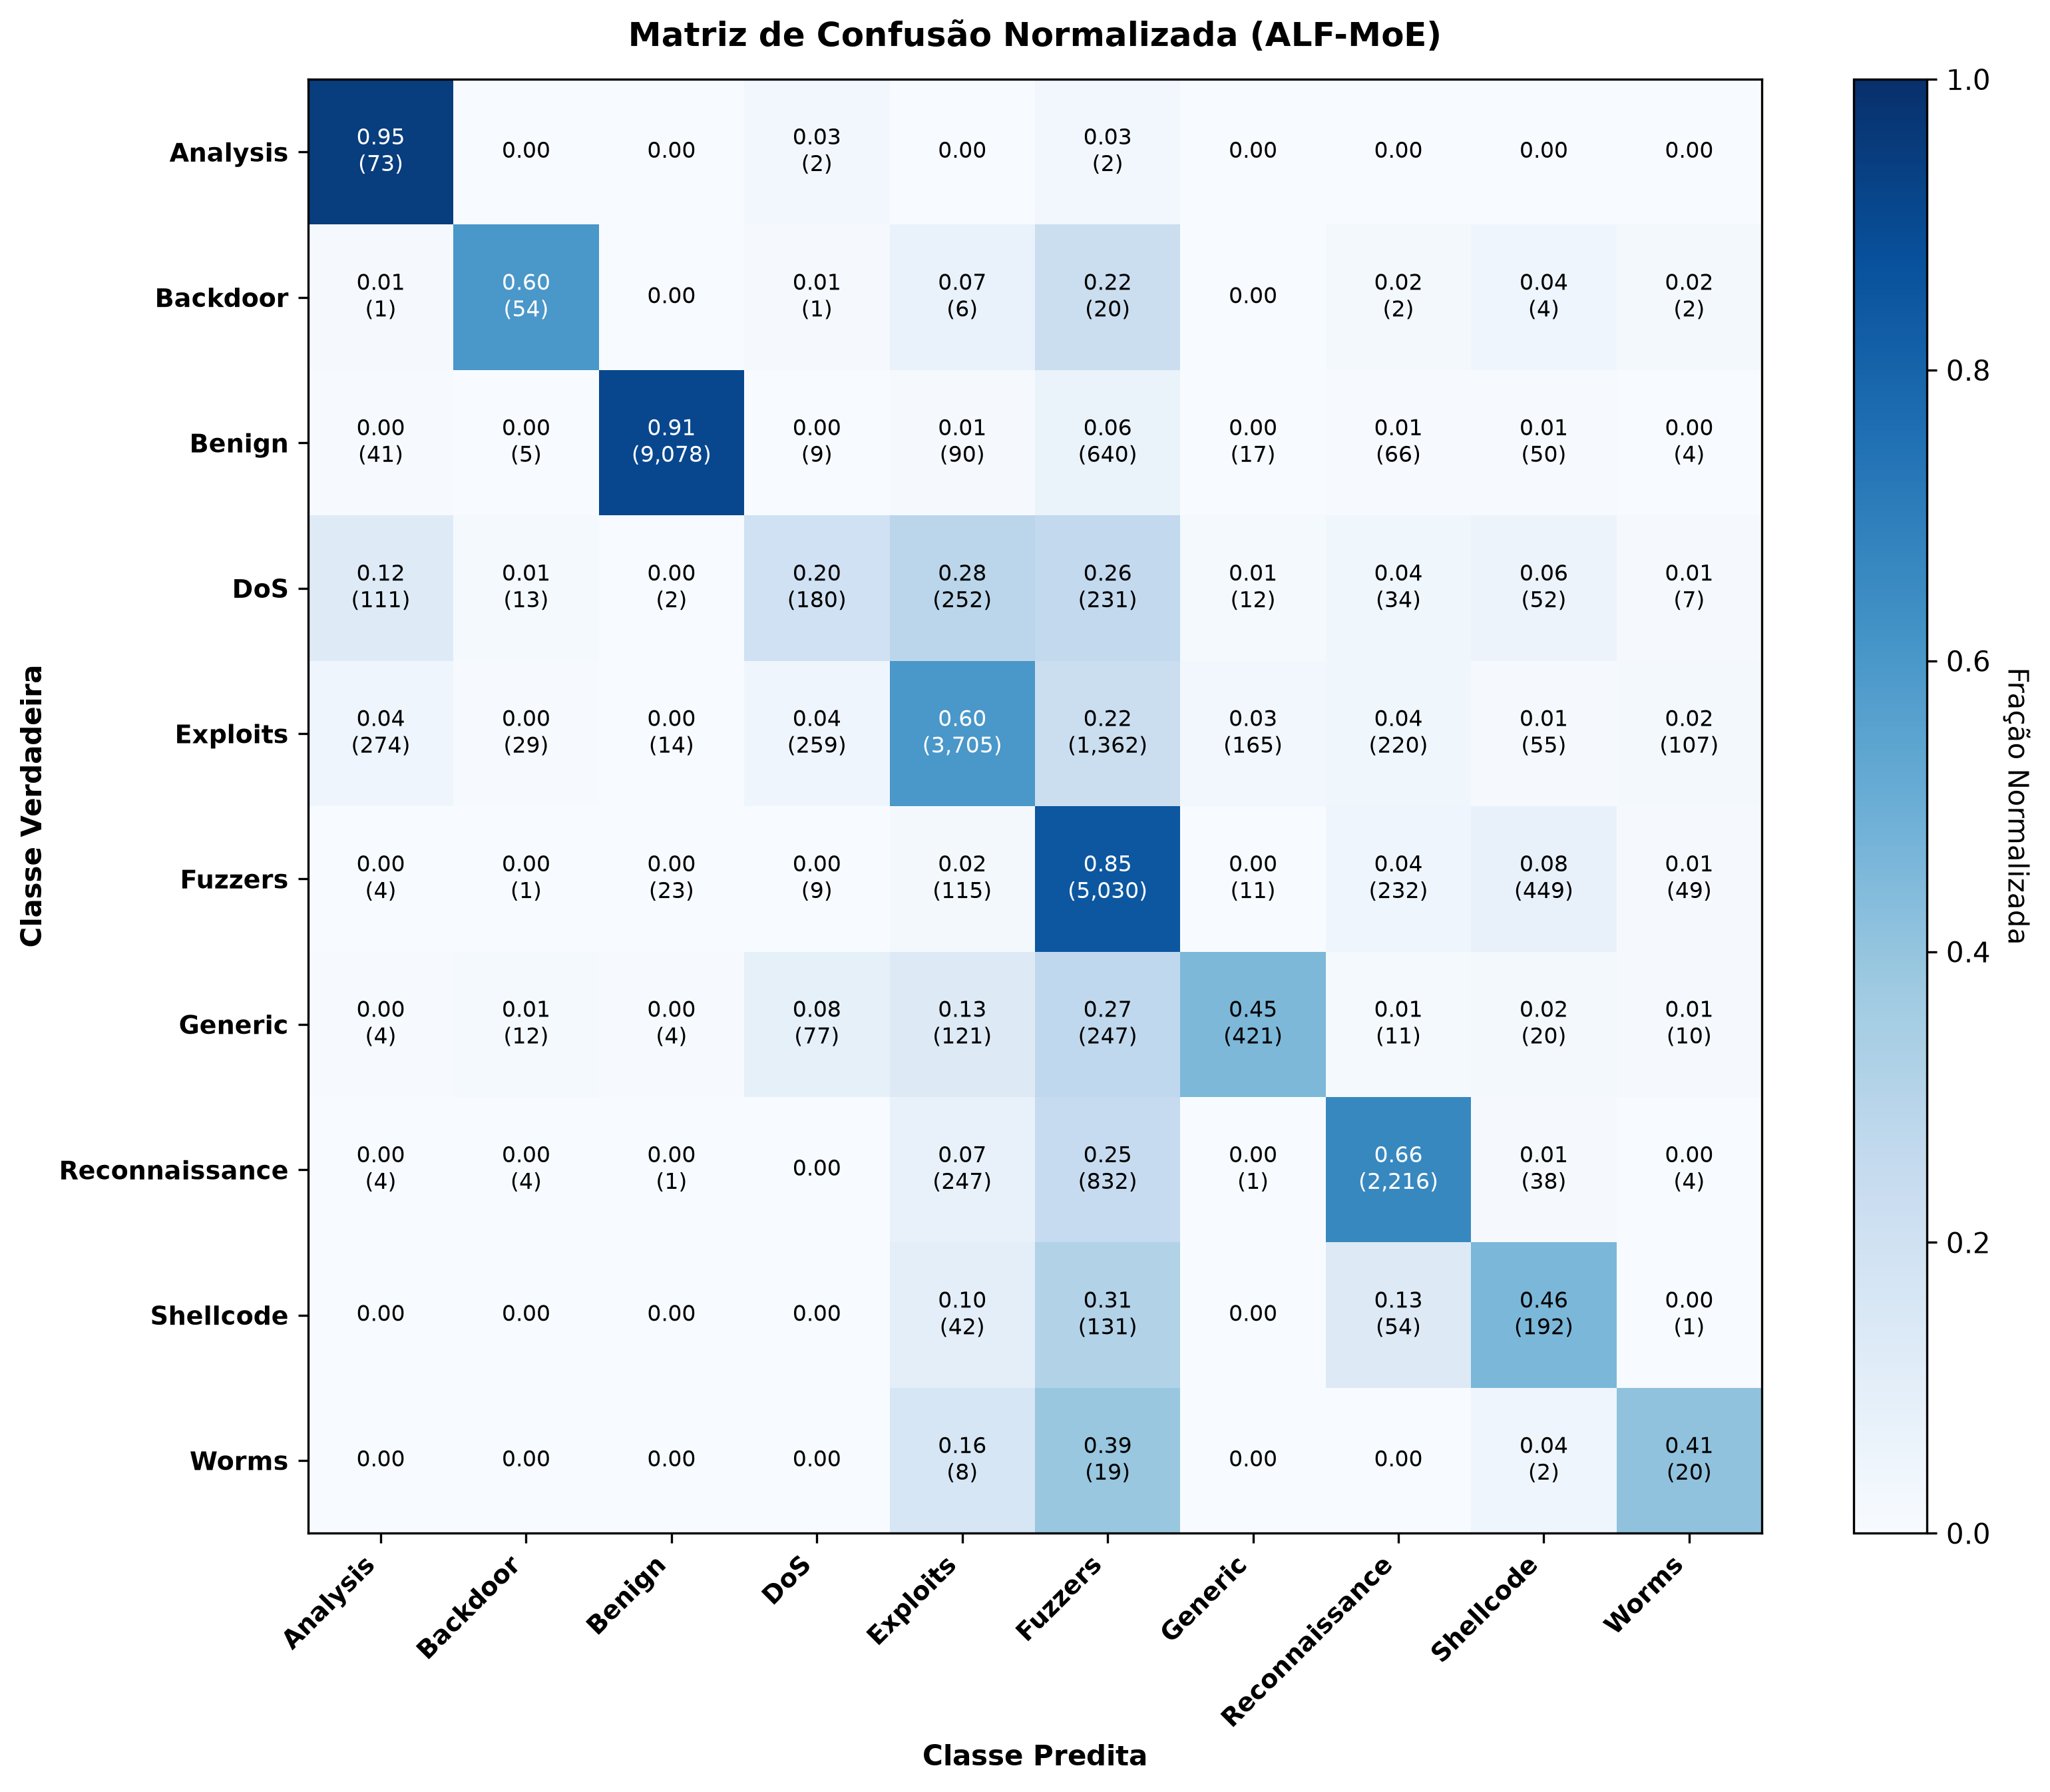
\includegraphics[width=\textwidth]{figures/benchmarks/cm_norm_unsw_l0.png}
    \caption{CIC-UNSW-NB15 (L0 - 10 classes).}
    \label{subfig:cm_unsw}
\end{subfigure}
\fonte{Elaborado pelo autor (2026), a partir dos artefatos de avaliação.}
\end{figure}

A inspeção visual confirma a dominância quase diagonal absoluta na versão corrigida do CSE-CIC-IDS2018 (Figura~\ref{subfig:cm_cse2018_imp}), em contraste com a dispersão de erros verificada na versão original (Figura~\ref{subfig:cm_cse2018_orig}). No ambiente IoT (Figura~\ref{subfig:cm_bccc2024}), observa-se perfeita segregação de tráfego de intermediadores MQTT ($96{,}0\%$ de acerto) e inundações DoS/DDoS ($>94\%$), enquanto o UNSW-NB15 (Figura~\ref{subfig:cm_unsw}) ilustra a sobreposição natural existente entre as classes \emph{Exploits} e \emph{Fuzzers}.

A análise pormenorizada das dispersões fora da diagonal principal permite fundamentar quatro padrões específicos de confusão interclasses observados nos experimentos, balizados pelas restrições físico-matemáticas da telemetria de fluxo:
\begin{enumerate}
    \item \textbf{CSE-CIC-IDS2018 Canônico (\emph{Infiltration} vs. \emph{WebAttack}):}
    Verifica-se sobreposição estatística mútua entre fluxos de infiltração e ataques a aplicações web. Essa confusão decorre do fato de ambos os vetores operarem predominantemente sobre os protocolos de transporte das portas 80 (HTTP) e 443 (HTTPS), compartilhando assinaturas idênticas de cabeçalho TCP e cadência de requisições. Como os extratores NetFlow/CICFlowMeter descartam o conteúdo da carga útil (\emph{payload}), a diferenciação apoia-se unicamente em distribuições de tamanho e temporização de pacotes. Além disso, a classe \emph{WebAttack} no conjunto canônico conta com suporte diminuto de teste (apenas 186 instâncias somando \emph{Brute Force - Web}, \emph{Brute Force - XSS} e \emph{SQL Injection}), limitando a estimativa das fronteiras bayesianas de decisão;
    
    \item \textbf{CSE-CIC-IDS2018 Corrigido (\emph{Benign} vs. \emph{Infiltration - Dropbox Download}):}
    Na base saneada conforme \citeonline{liu2022error}, a classe \emph{Infiltration - Dropbox Download} alcança $F_1 = 0{,}1818$ com dispersão preponderante em direção à classe \emph{Benign}. Essa confusão é tecnicamente inevitável no nível de fluxo: a exfiltração de dados e download de artefatos maliciosos via API oficial do Dropbox utiliza canais TLS legítimos em conexões HTTPS padronizadas, reproduzindo rigorosamente as grandezas estatísticas e temporais da navegação web corporativa. Aliado ao suporte ultra-reduzido de apenas 17 amostras de teste, esse vetor atinge o limite intrínseco de separabilidade de extratores estritamente baseados em fluxo de rede;
    
    \item \textbf{CIC-BCCC-NRC TabularIoTAttack-2024 (\emph{MITM} vs. \emph{Botnet}):}
    No ecossistema IoT, constata-se confusão pontual entre fluxos das macro-famílias \emph{MITM} (especialmente variantes de \emph{ARP Spoofing}) e tráfego de \emph{Botnet}. Em redes locais de sensores e atuadores, ambos os vetores caracterizam-se por mensagens curtas de controle TCP/IP, ausência de fluxos volumétricos em rajada (\emph{bulk}) e temporizações assíncronas com intervalos de inter-chegada assemelhados, induzindo dispersão correlacionada nos logits da Gating Network;
    
    \item \textbf{CIC-UNSW-NB15 (\emph{Analysis}, \emph{Backdoor}, \emph{Exploits} e \emph{Fuzzers}):}
    No benchmark UNSW-NB15, verifica-se sobreposição estatística mútua entre as classes \emph{Exploits} ($22{,}17\%$ do teste) e \emph{Fuzzers} ($21{,}22\%$), além de falsos positivos cruzados com \emph{Analysis} e \emph{Backdoor}. Conforme documentado por \citeonline{moustafa2015unsw}, o tráfego sintético dessa base foi sintetizado pelo gerador de hardware comercial IXIA PerfectStorm injetando transações HTTP padronizadas com payloads mutacionados. No plano da telemetria de fluxo (contadores agregados de pacotes, bytes e intervalos IAT), essas classes produzem vetores numéricos virtualmente idênticos, delimitando um teto teórico de erro de Bayes intransponível sem inspeção profunda de pacotes (DPI).
\end{enumerate}


\subsection{Análise Comparativa dos Especialistas e do Bloco ALF}
\label{subsec:estudo_ablacao}

A arquitetura ALF-MoE apoia-se no princípio de que especialistas neurais heterogêneos, concebidos para extrair representações de domínios específicos da telemetria de rede, oferecem projeções complementares que, ao serem integradas pela fusão por atenção adaptativa, superam a capacidade preditiva de qualquer modelo monolítico individual. Para quantificar essa premissa de projeto e mensurar o ganho advindo do bloco atencional ALF sobre os ramos isolados, realizou-se uma análise comparativa sistemática entre as predições supervisionadas das cinco cabeças especializadas ($\mathcal{E}_{\mathrm{DNN}}, \mathcal{E}_{\mathrm{CNN}}, \mathcal{E}_{\mathrm{GRU}}, \mathcal{E}_{\mathrm{CAE}}, \mathcal{E}_{\mathrm{LSTM}}$) e a predição da cabeça integrada ALF-MoE.

A Tabela~\ref{tab:estudo_ablacao_completo} sumariza o Macro $F_1$-Score e a Acurácia Global obtidos por cada especialista e pela cabeça unificada ALF nos sete cenários de teste.

\begin{table}[htb]
\centering
\caption{Estudo de ablação: Macro $F_1$-Score e Acurácia dos especialistas individuais vs. ALF-MoE.}
\label{tab:estudo_ablacao_completo}
\footnotesize
\setlength{\tabcolsep}{4.5pt}
\begin{tabularx}{\textwidth}{>{\raggedright\arraybackslash}X l rrrrrr}
\hline
\textbf{Dataset} & \textbf{Métrica} & \textbf{DNN} & \textbf{CNN} & \textbf{GRU} & \textbf{CAE} & \textbf{LSTM} & \textbf{ALF-MoE} \\
\hline
\multirow{2}{*}{CIC-UNSW-NB15 (L0)} 
 & Macro $F_1$ & 0,4611 & 0,4053 & 0,4367 & 0,2525 & 0,2779 & \textbf{0,5069} \\
 & Acurácia    & 71,77\% & 58,56\% & 71,42\% & 62,28\% & 64,12\% & \textbf{75,11\%} \\
\hline
\multirow{2}{*}{CIC-BCCC-NRC-2024 (L0)} 
 & Macro $F_1$ & 0,0057 & 0,2496 & 0,4448 & 0,1246 & 0,3676 & \textbf{0,4501} \\
 & Acurácia    & 10,88\% & 41,31\% & \textbf{82,33\%} & 60,73\% & 80,06\% & 82,29\% \\
\hline
\multirow{2}{*}{CIC-BCCC-NRC-2024 (L2)} 
 & Macro $F_1$ & 0,1284 & 0,5551 & 0,8451 & 0,2557 & 0,8163 & \textbf{0,8476} \\
 & Acurácia    & 12,41\% & 57,04\% & 92,26\% & 60,55\% & 90,88\% & \textbf{92,83\%} \\
\hline
\multirow{2}{*}{CSE-CIC-IDS2018 Orig. (L0)} 
 & Macro $F_1$ & 0,7588 & 0,5485 & 0,7681 & 0,4750 & 0,6891 & \textbf{0,8773} \\
 & Acurácia    & 93,05\% & 51,73\% & 88,62\% & 69,61\% & 89,09\% & \textbf{98,96\%} \\
\hline
\multirow{2}{*}{CSE-CIC-IDS2018 Orig. (L2)} 
 & Macro $F_1$ & 0,8442 & 0,5925 & 0,8181 & 0,3029 & 0,7880 & \textbf{0,9050} \\
 & Acurácia    & 94,30\% & 61,53\% & 88,62\% & 44,05\% & 88,13\% & \textbf{98,38\%} \\
\hline
\multirow{2}{*}{CSE-CIC-IDS2018 Corr. (L0)} 
 & Macro $F_1$ & 0,7862 & 0,7156 & 0,8390 & 0,4405 & 0,7598 & \textbf{0,8918} \\
 & Acurácia    & 99,85\% & 92,87\% & 99,40\% & 78,51\% & 98,37\% & \textbf{99,97\%} \\
\hline
\multirow{2}{*}{CSE-CIC-IDS2018 Corr. (L2)} 
 & Macro $F_1$ & 0,8134 & 0,6953 & 0,8464 & 0,5115 & 0,7344 & \textbf{0,8851} \\
 & Acurácia    & 99,85\% & 92,84\% & 99,34\% & 77,40\% & 97,77\% & \textbf{99,96\%} \\
\hline
\end{tabularx}
\fonte{Elaborado pelo autor (2026), com base nos relatórios de teste.}
\end{table}

A análise minuciosa da Tabela~\ref{tab:estudo_ablacao_completo} permite derivar conclusões estruturais acerca do comportamento dos especialistas e do ganho proporcionado pela fusão ALF:
\begin{enumerate}
    \item \textbf{Superação Sistemática do Melhor Especialista Individual:}
    Em todos os cenários sem exceção, a fusão atencional \textbf{ALF-MoE} alcança o melhor Macro $F_1$-Score global. No CIC-UNSW-NB15, o melhor especialista isolado foi a $\mathcal{E}_{\mathrm{DNN}}$ ($F_1 = 0{,}4611$), enquanto o ALF-MoE atingiu $0{,}5069$ (ganho de $+4{,}58$ pontos percentuais de $F_1$ e $+3{,}34\%$ em acurácia). No CSE-CIC-IDS2018 Canônico (L0), o ganho é ainda mais acentuado: o melhor especialista individual foi a $\mathcal{E}_{\mathrm{GRU}}$ com $F_1 = 0{,}7681$, superada largamente pelo ALF-MoE com $0{,}8773$ (um salto de $+10{,}92$ pontos de $F_1$ e $+5{,}91\%$ de acurácia sobre a DNN);
    
    \item \textbf{Especialização Funcional por Domínio:}
    Os especialistas $\mathcal{E}_{\mathrm{GRU}}$ e $\mathcal{E}_{\mathrm{LSTM}}$, encarregados da telemetria de intervalos temporais (\emph{IAT} e \emph{Active/Idle}), demonstraram liderança folgada no tráfego IoT (CIC-BCCC-NRC-2024), alcançando $F_1$ de $0{,}8451$ e $0{,}8163$, respectivamente, enquanto os modelos alimentados unicamente por propriedades de pacotes ou globais sofreram degradação. Isso decorre da natureza do protocolo MQTT, cujos pacotes apresentam tamanho uniforme de cabeçalho, tornando os padrões de tempo entre chegadas o elemento primordial de discriminação;
    
    \item \textbf{Papel Regularizador do Autoencoder Convolucional ($\mathcal{E}_{\mathrm{CAE}}$):}
    Embora o $\mathcal{E}_{\mathrm{CAE}}$ isole pontuações mais modestas como classificador autônomo (variando entre $F_1 = 0{,}1246$ e $0{,}5115$), sua inclusão no grafo computacional provê uma restrição de reconstrução espectral no domínio da frequência ($\mathcal{L}_{\mathrm{CAE\_rec}}$) que atua como regularizador indutivo, impedindo que os especialistas densos entrem em colapso latente diante de fluxos volumétricos colineares.
\end{enumerate}

\subsubsection{Gráficos Radar de Especialistas}

A complementaridade multidomínio dos modelos é visualizada na Figura~\ref{fig:radar_especialistas_painel}, que reúne os gráficos radar de comparação entre cada especialista e a arquitetura ALF-MoE nos quatro conjuntos de teste.

\begin{figure}[htb]
\centering
\caption{Gráficos radar comparativos de desempenho por classe: Especialistas individuais vs. ALF-MoE.}
\label{fig:radar_especialistas_painel}
\begin{subfigure}[b]{0.48\textwidth}
    \centering
    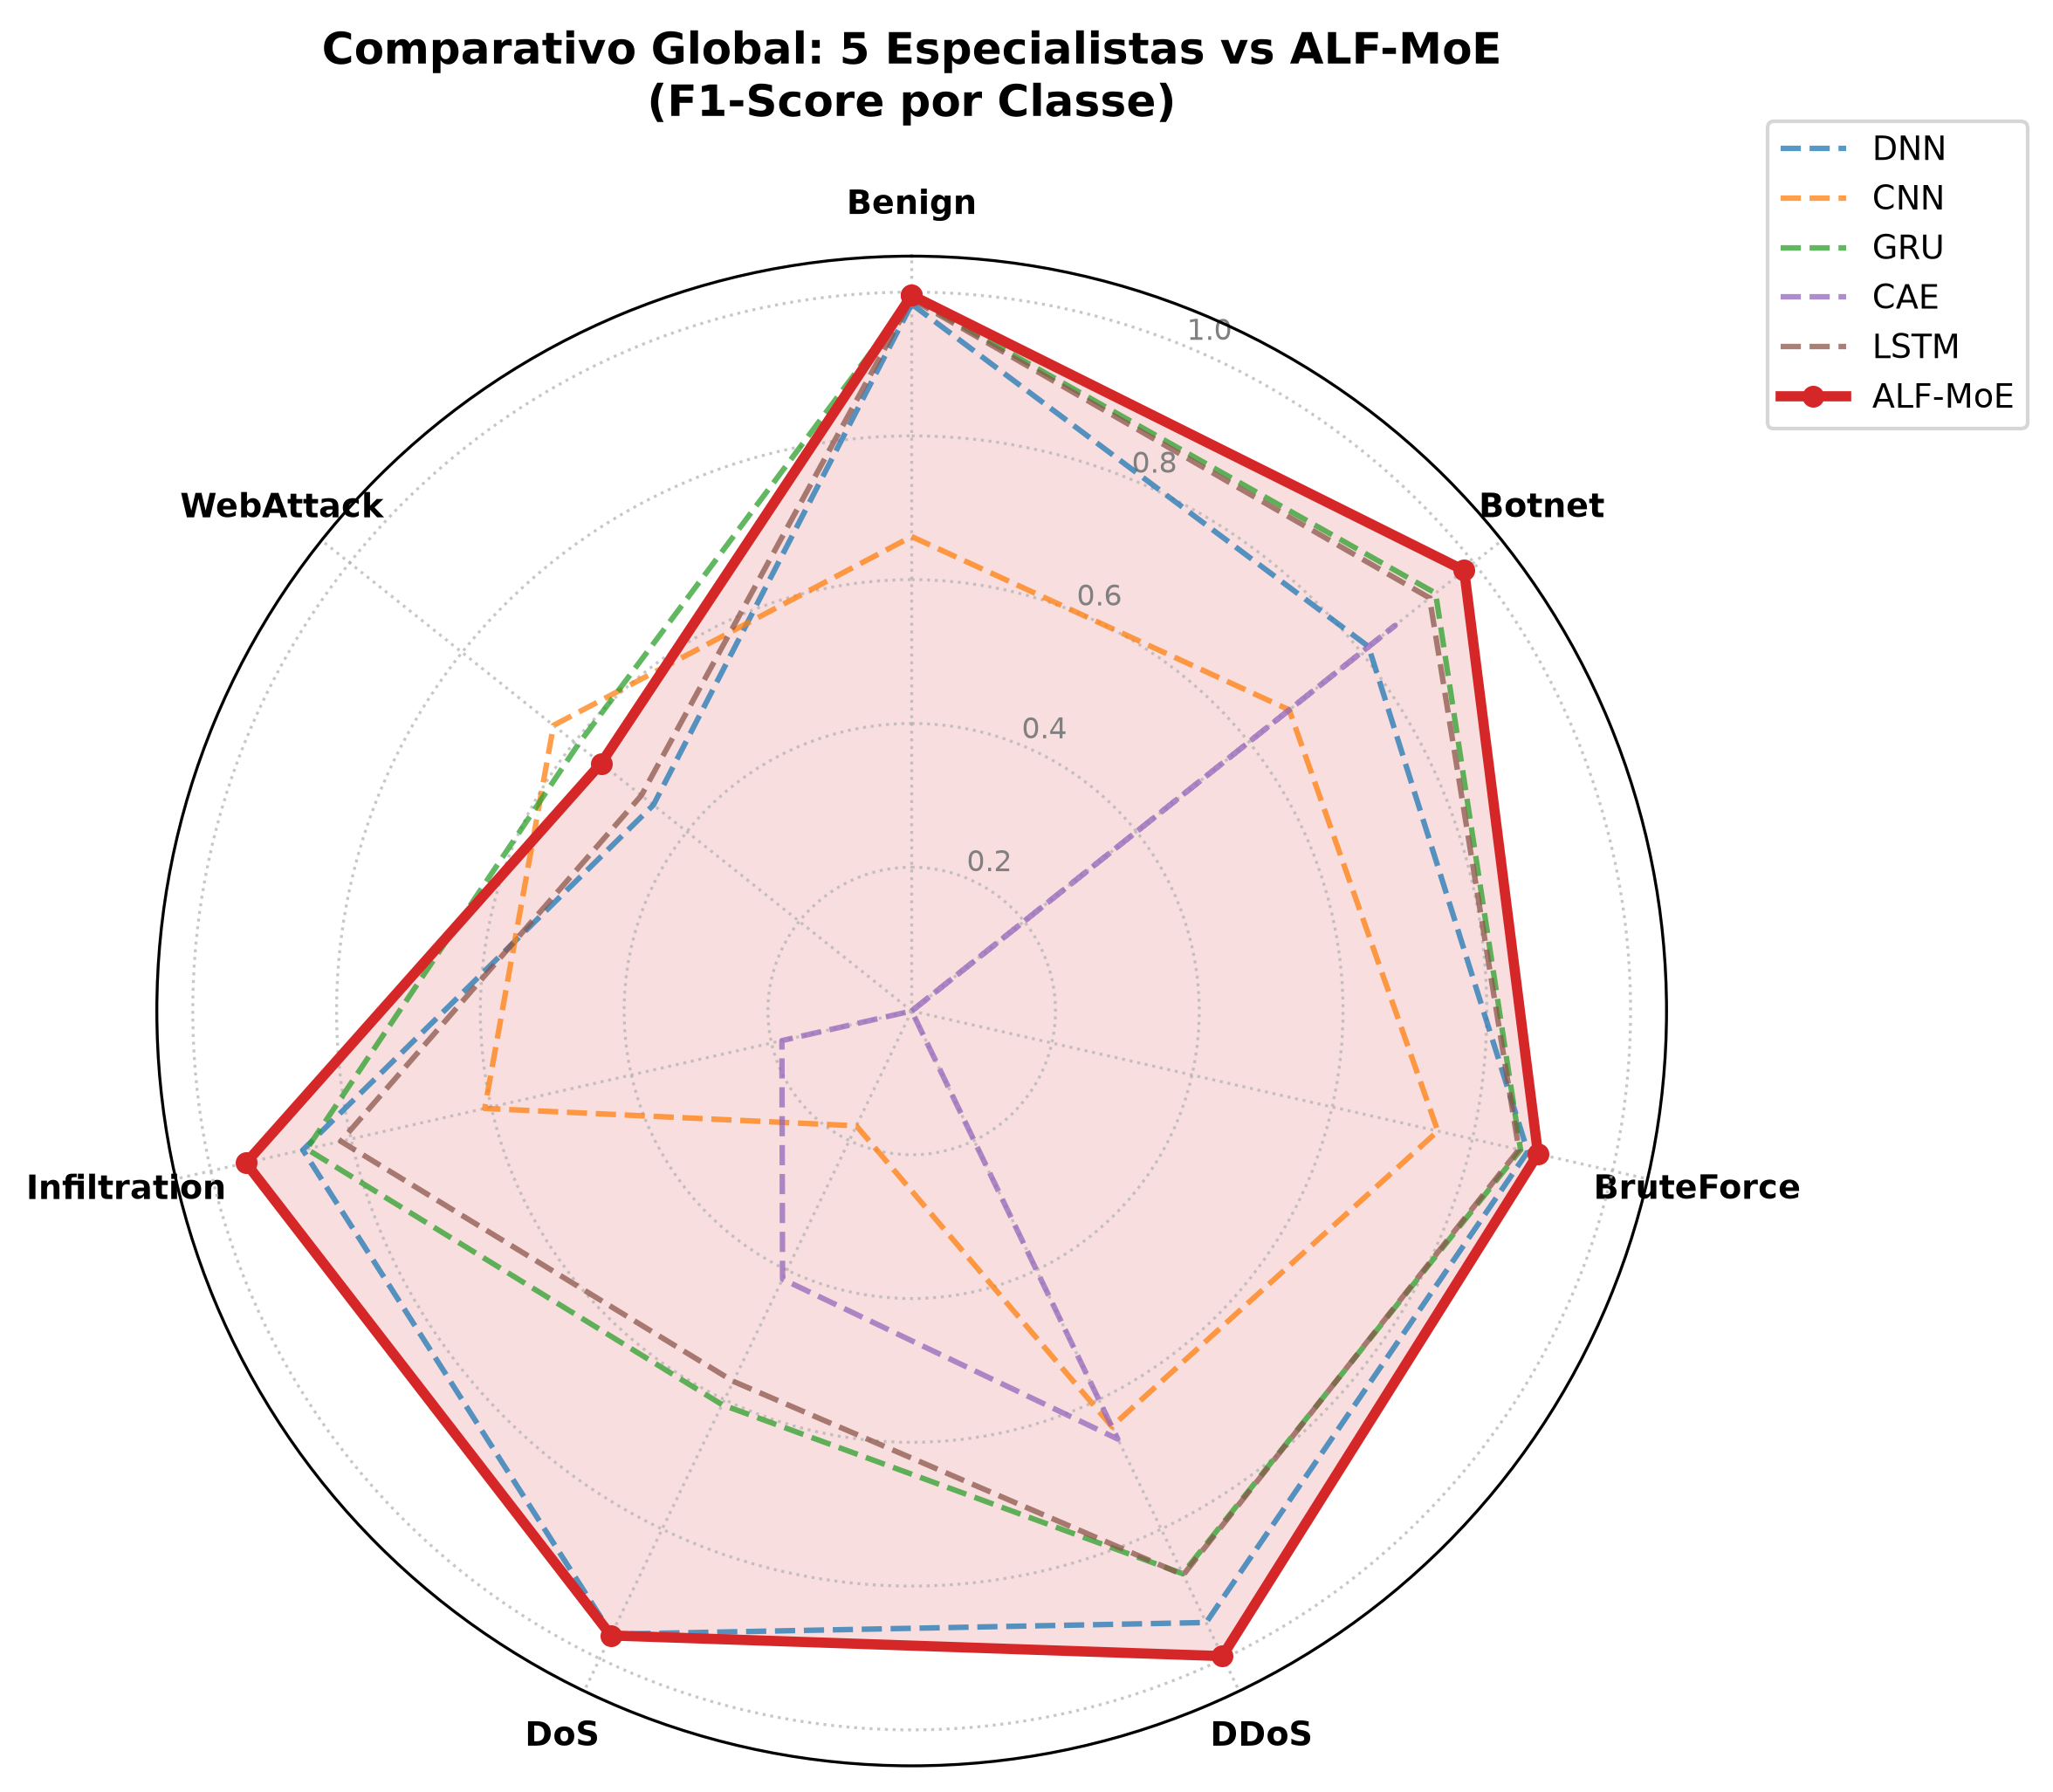
\includegraphics[width=\textwidth]{figures/benchmarks/radar_cse2018_l2.png}
    \caption{CSE-CIC-IDS2018 Canônico (L2).}
    \label{subfig:radar_cse_orig}
\end{subfigure}
\hfill
\begin{subfigure}[b]{0.48\textwidth}
    \centering
    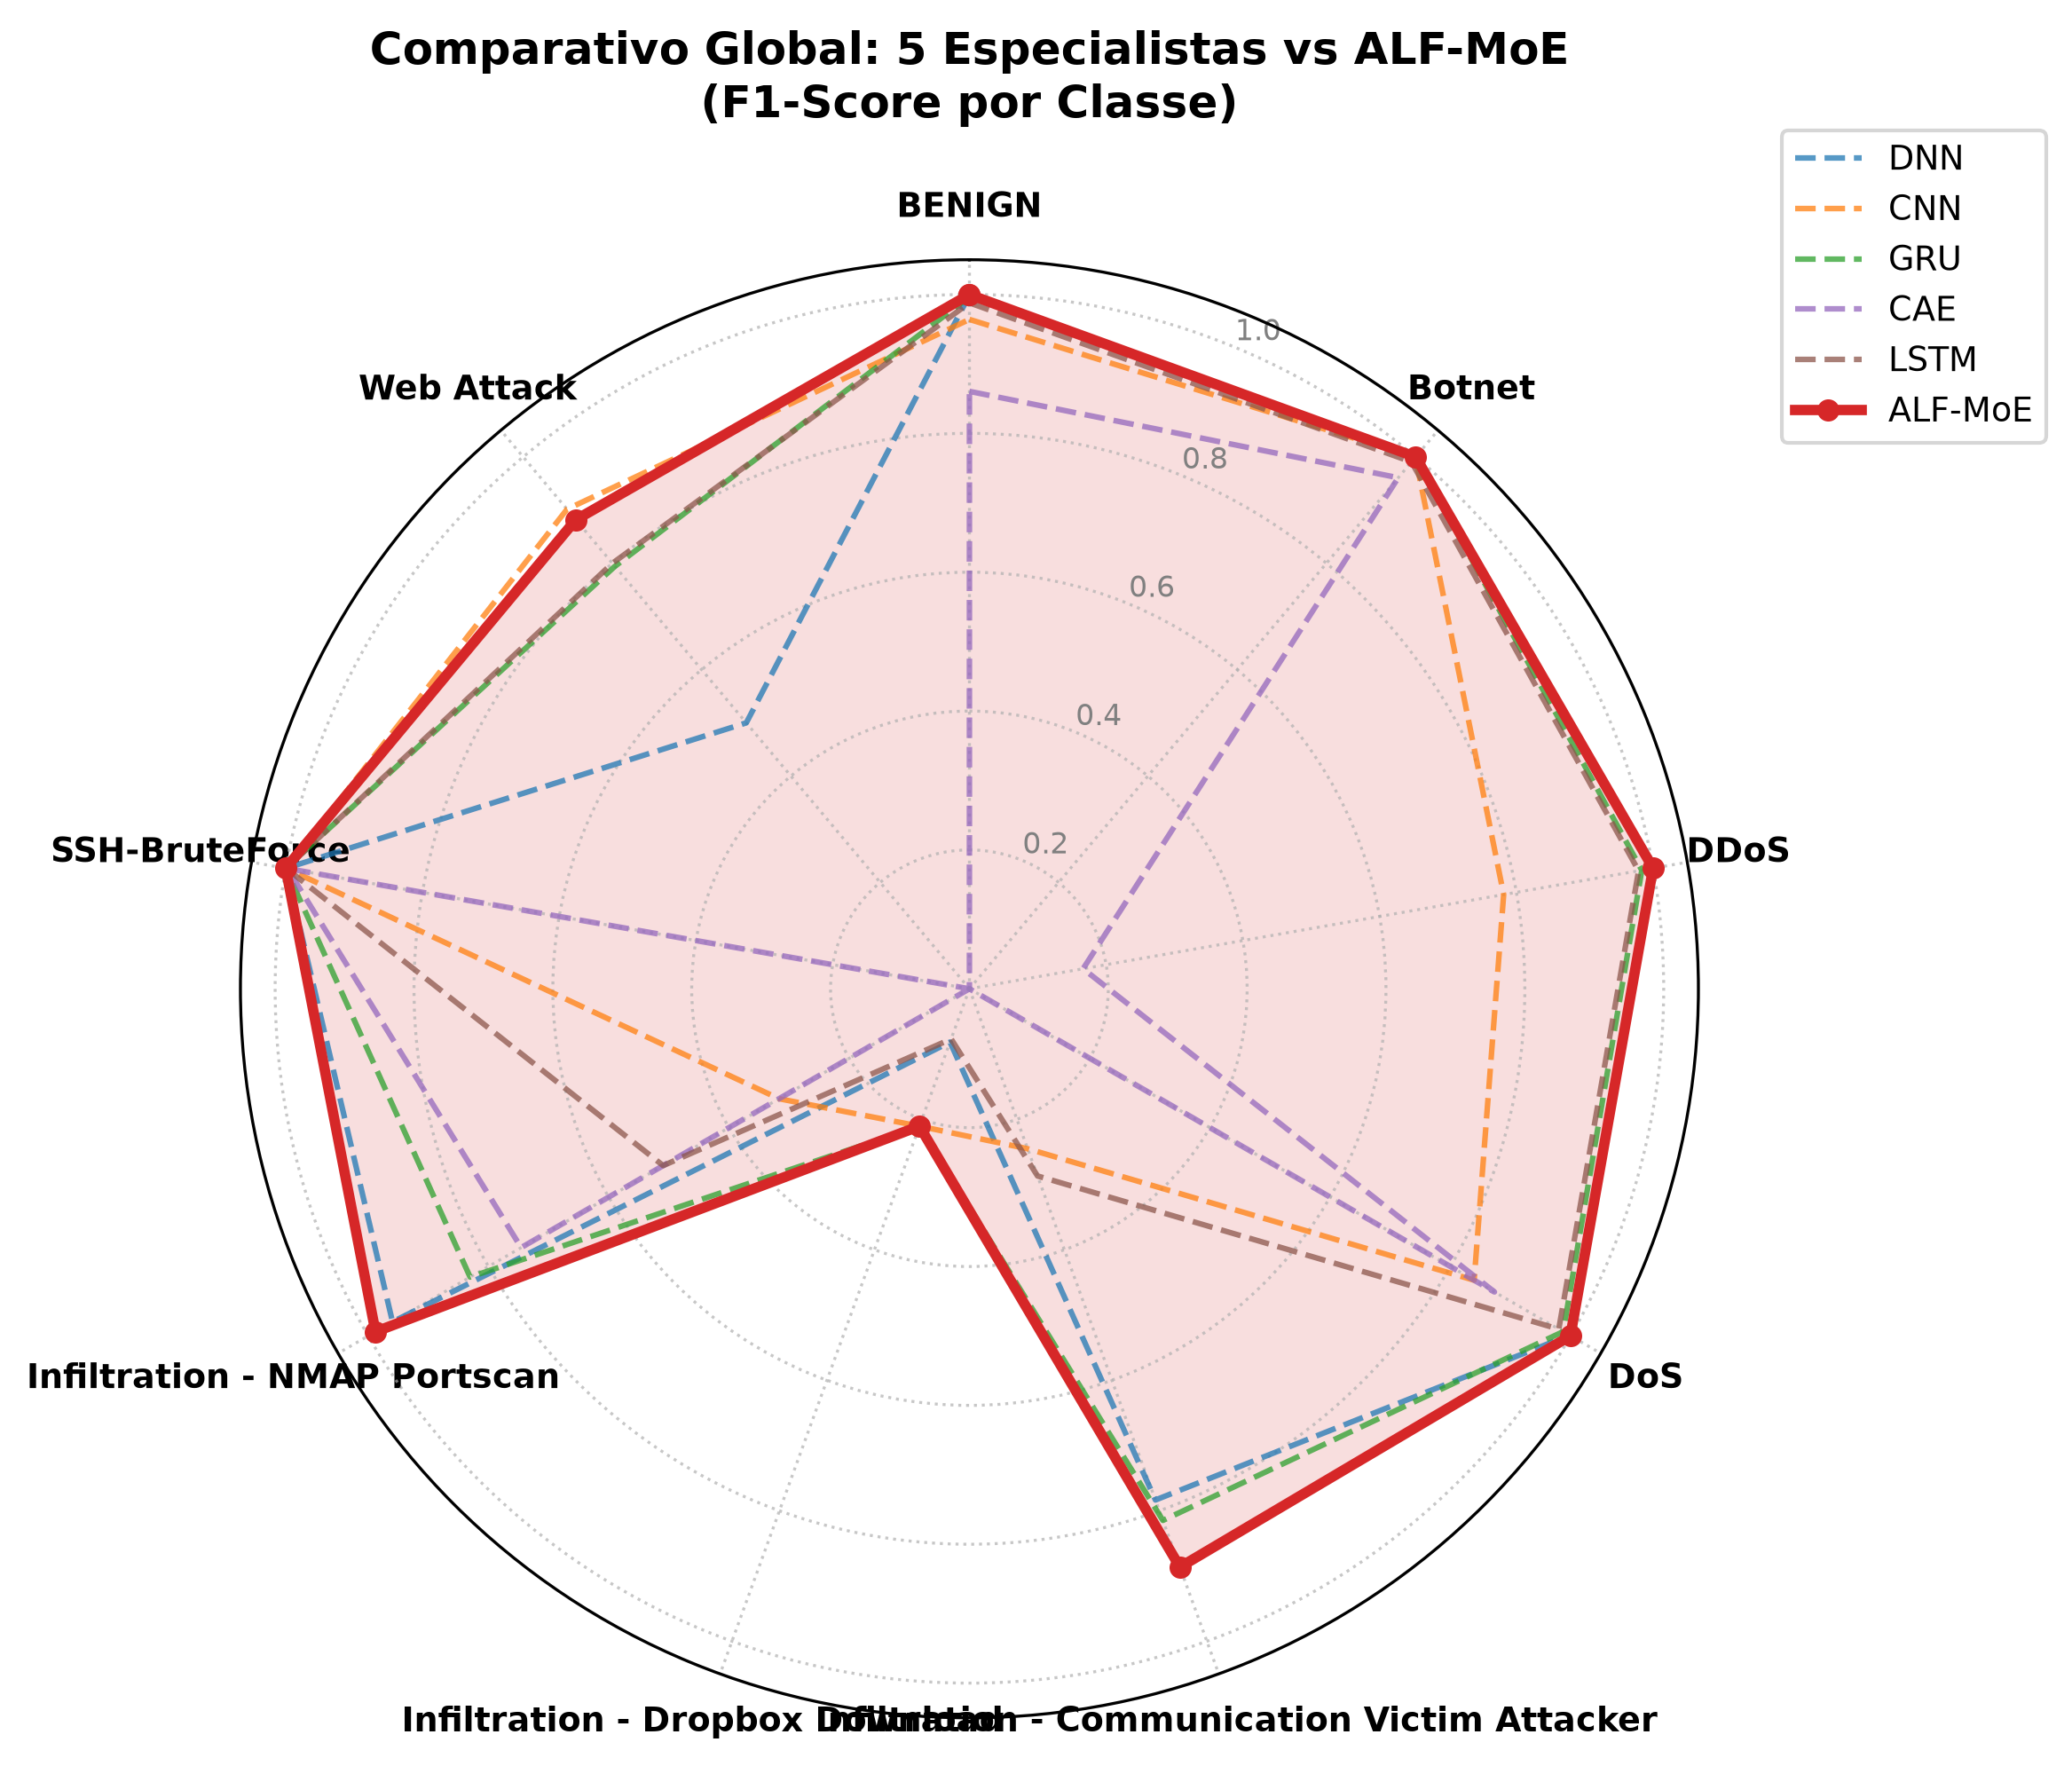
\includegraphics[width=\textwidth]{figures/benchmarks/radar_cse2018_imp_l2.png}
    \caption{CSE-CIC-IDS2018 Corrigido (L2).}
    \label{subfig:radar_cse_imp}
\end{subfigure}

\vspace{0.4cm}

\begin{subfigure}[b]{0.48\textwidth}
    \centering
    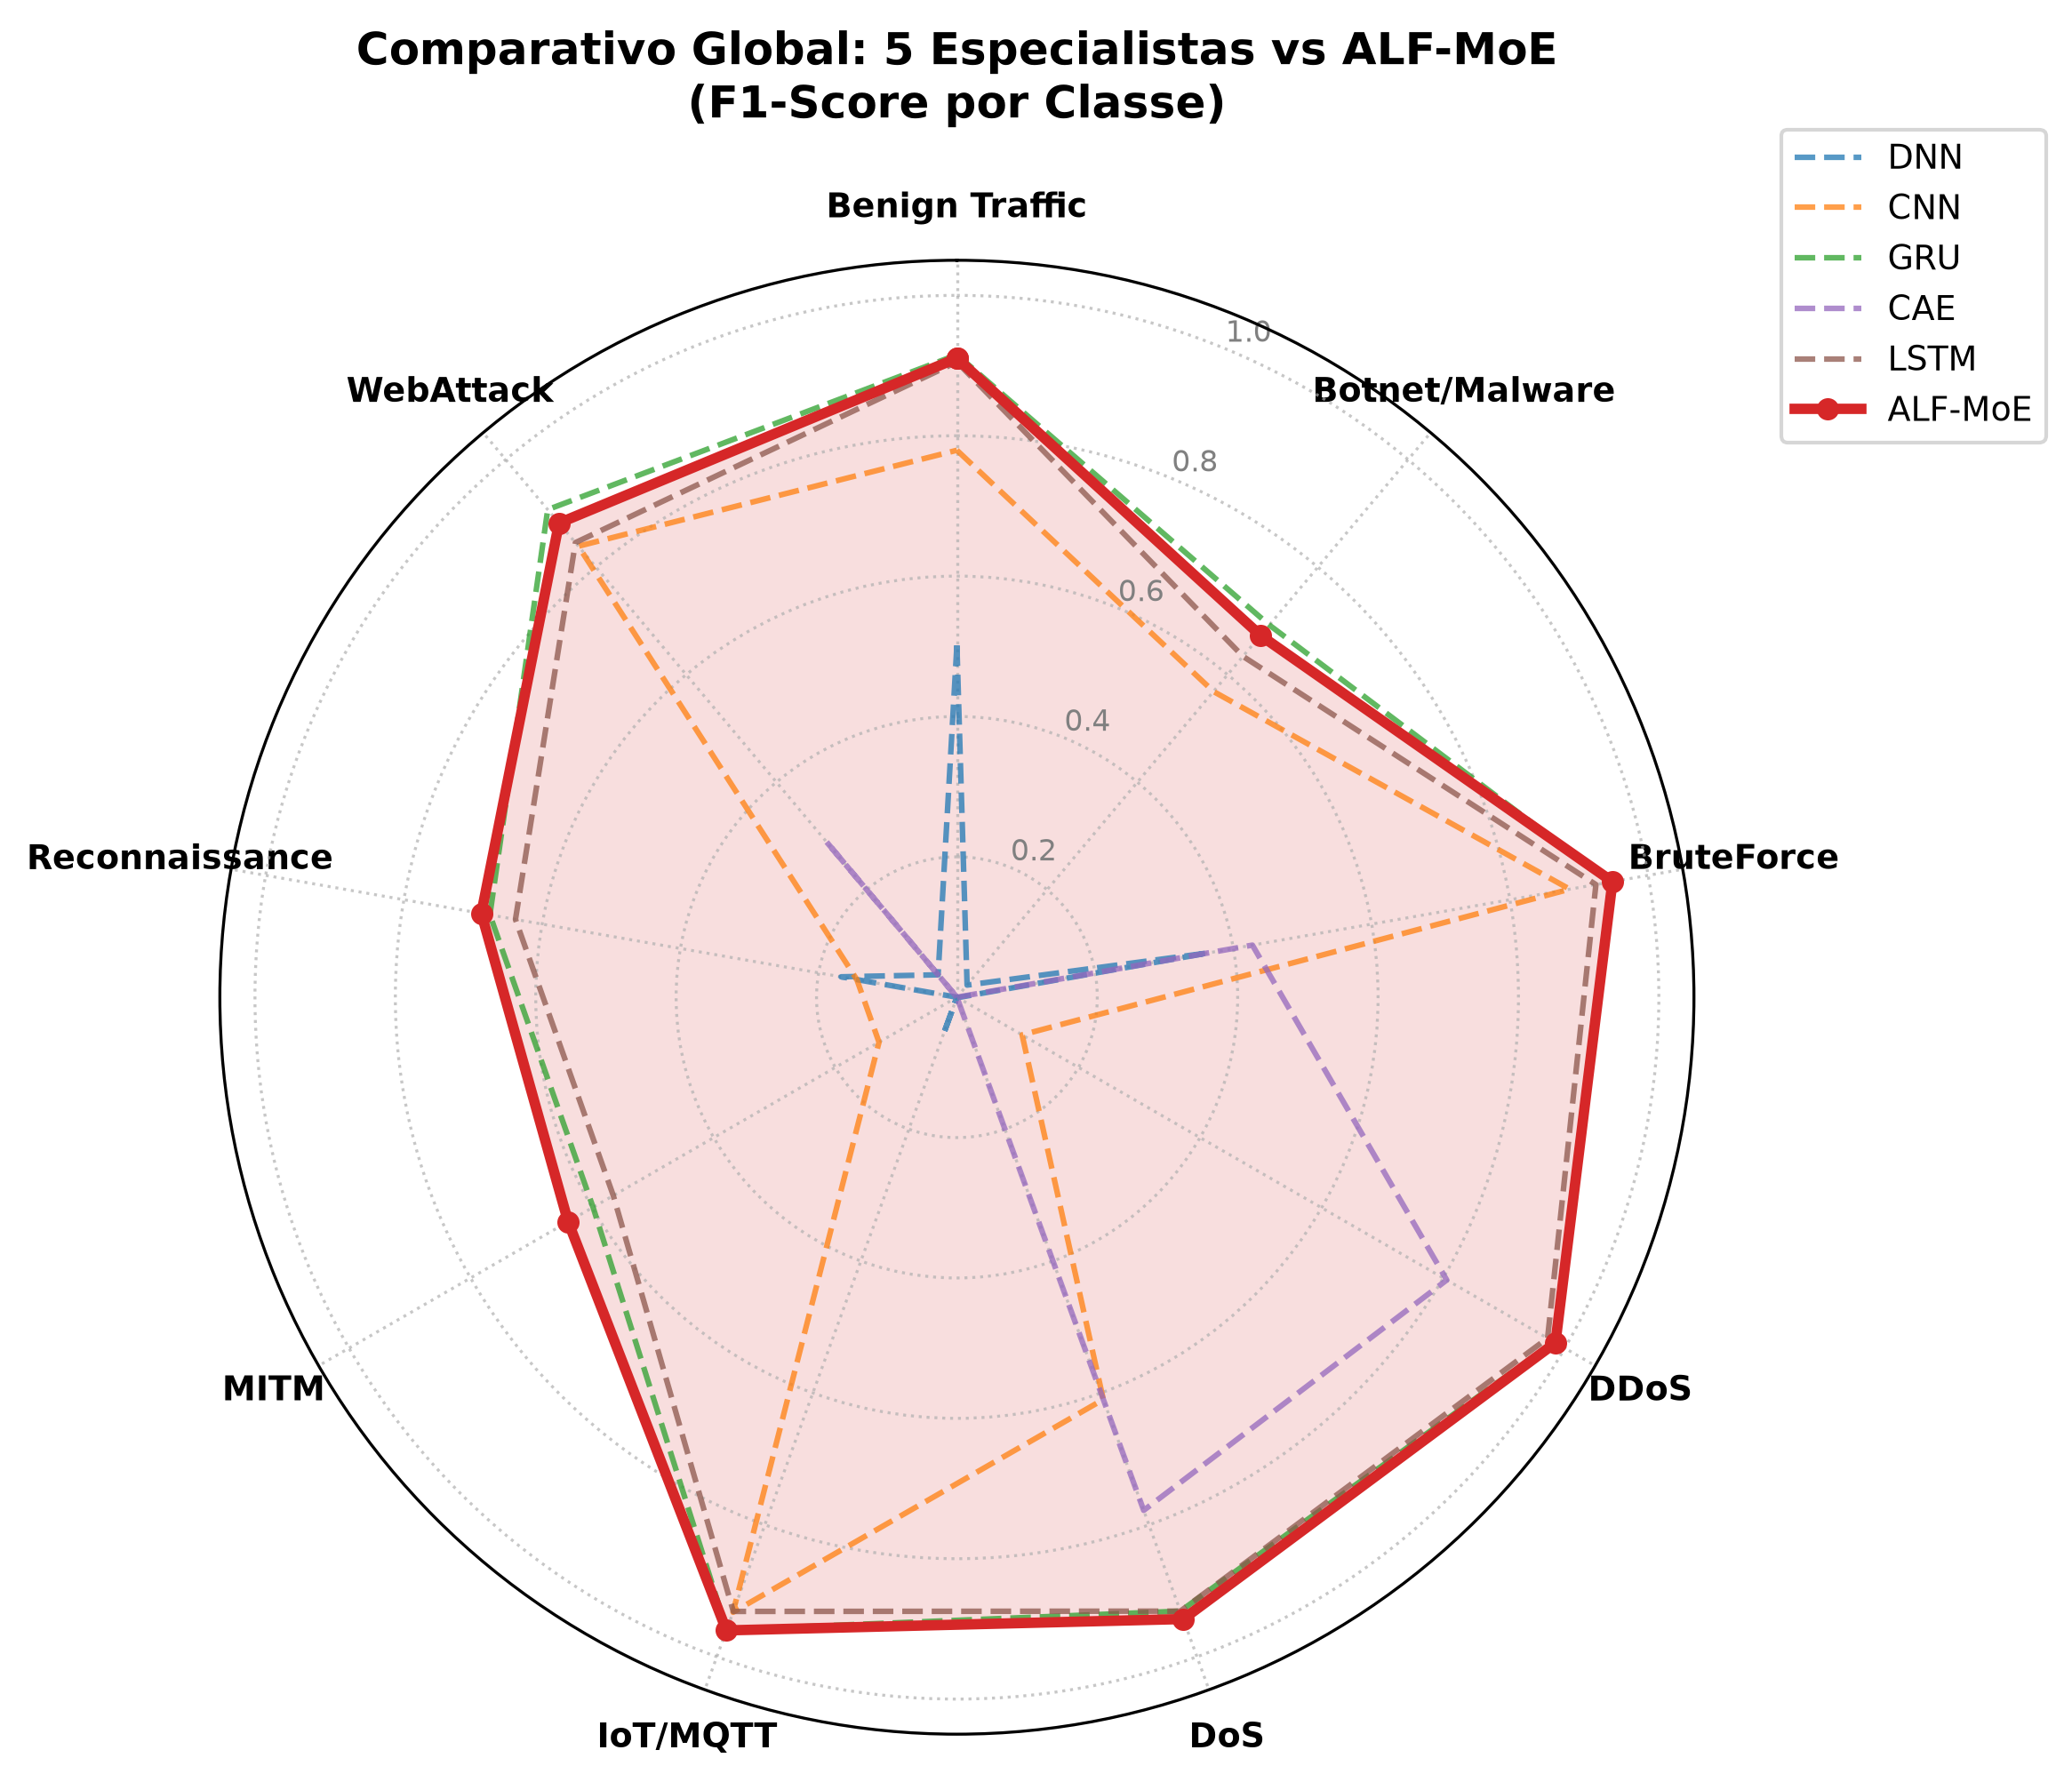
\includegraphics[width=\textwidth]{figures/benchmarks/radar_bccc2024_l2.png}
    \caption{CIC-BCCC-NRC-2024 (L2).}
    \label{subfig:radar_bccc}
\end{subfigure}
\hfill
\begin{subfigure}[b]{0.48\textwidth}
    \centering
    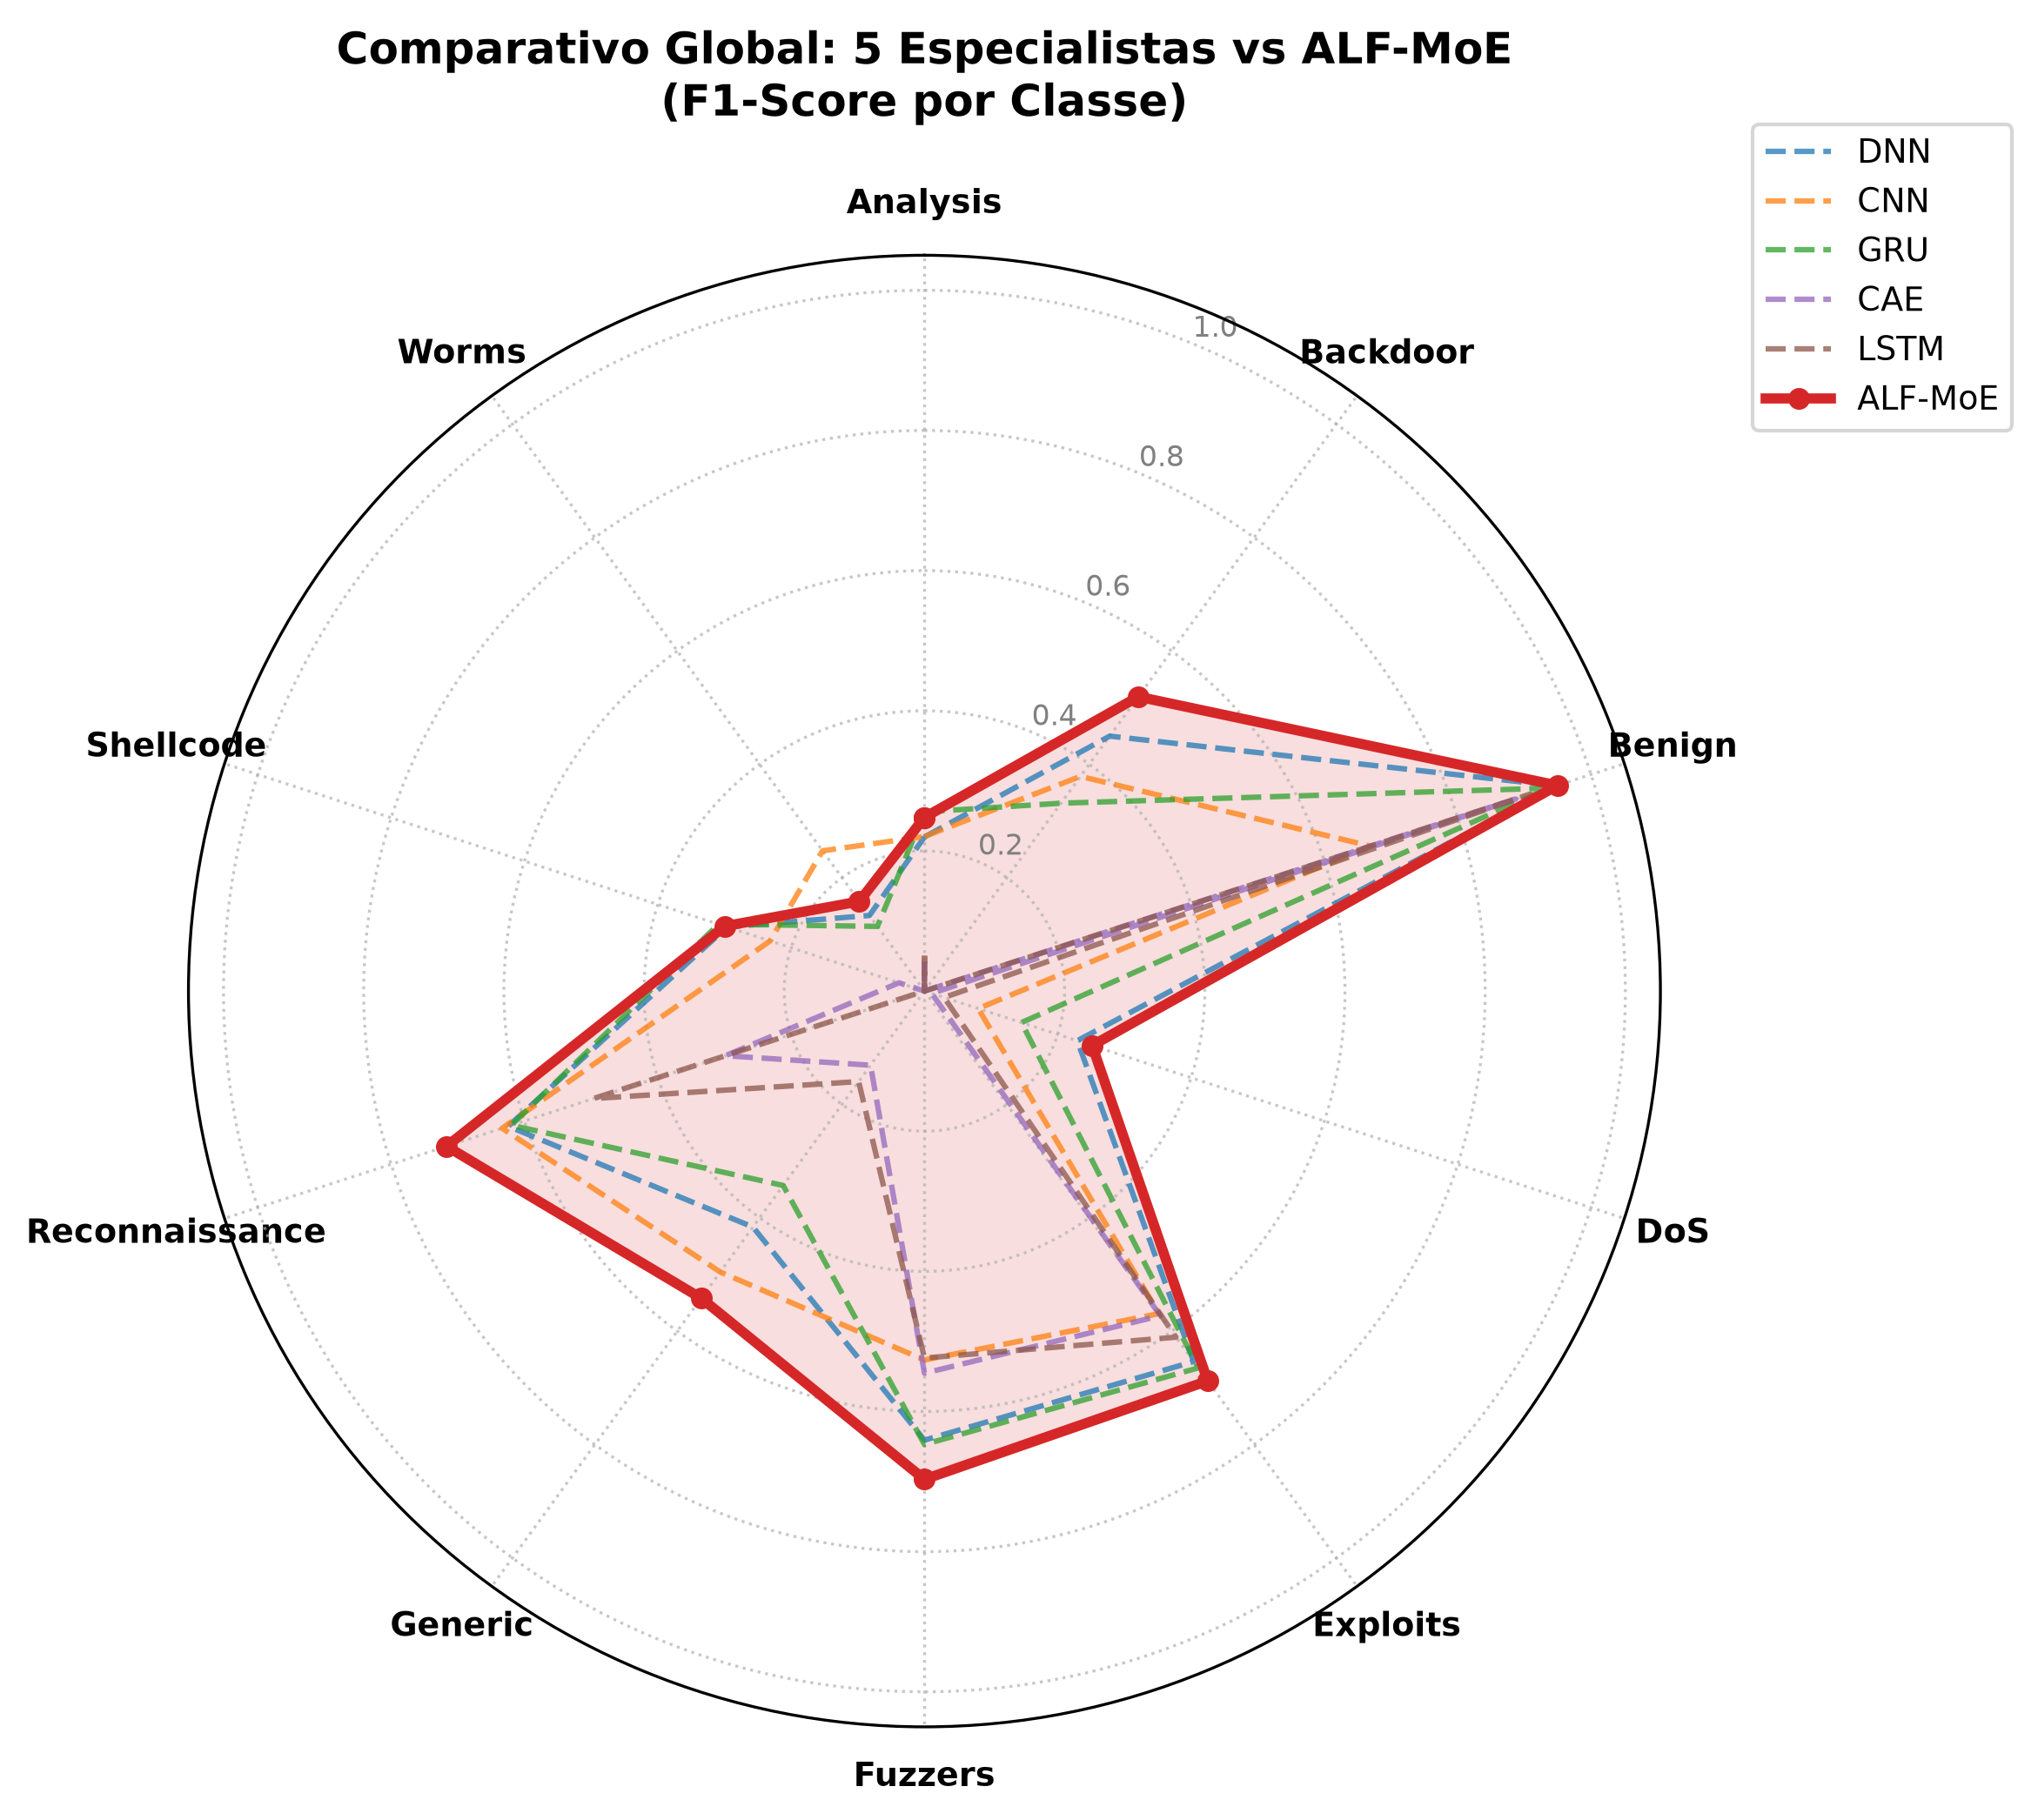
\includegraphics[width=\textwidth]{figures/benchmarks/radar_unsw_l0.png}
    \caption{CIC-UNSW-NB15 (L0).}
    \label{subfig:radar_unsw}
\end{subfigure}
\fonte{Elaborado pelo autor (2026), a partir dos artefatos de avaliação.}
\end{figure}

Em todas as representações radiais da Figura~\ref{fig:radar_especialistas_painel}, o polígono correspondente ao **ALF-MoE** (em linha de destaque) delimita a envoltória superior em virtualmente todas as direções de ataque. Mesmo quando um especialista específico exibe deficiência em um determinado vetor (por exemplo, a queda acentuada da DNN em classes IoT ou da CNN em ataques de força bruta), o mecanismo de fusão atencional redistribui dinamicamente os pesos para os especialistas mais bem capacitados, demonstrando a robustez teórica e prática do projeto ALF-MoE.


\section{Avaliação da Extração e Inferência em Tráfego Real/PCAPs}
\label{sec:avaliacao_extracao_inferencia}

A transição de modelos de Aprendizado Profundo avaliados em partições estáticas de \emph{benchmark} para pipelines operacionais de inspeção de rede em tempo real impõe severos desafios de engenharia de software e processamento de sinais. Enquanto a avaliação \emph{offline} assume dados pré-segmentados, normalizados e perfeitamente indexados, o ambiente de produção lida com fluxos bidirecionais concorrentes, assincronia de eventos, variações de temporização de \emph{hardware} e restrições de latência determinística. Esta seção examina o comportamento do arcabouço **ALF-MoE** quando implantado em bancada física real, analisando a fidelidade da extração de características em tempo real via NFStream, o perfil de consumo de recursos computacionais e os gargalos estruturais de latência ponta a ponta.


\subsection{Impacto do Mapeamento NFStream \texorpdfstring{$\to$}{->} CICFlowMeter}
\label{subsec:impacto_mapeamento}

Os conjuntos de dados de referência utilizados no treinamento supervisionado do ALF-MoE (notadamente CSE-CIC-IDS2018, CIC-UNSW-NB15 e CIC-BCCC-NRC-2024) foram originalmente gerados por meio do extrator proprietário \emph{CICFlowMeter} \cite{Sharafaldin2018TowardGA}, uma aplicação monolítica escrita em Java que processa arquivos de captura (.pcap) de forma puramente \emph{offline}. Para viabilizar a inferência em tempo de execução na interface de rede da máquina vítima, concebeu-se um pipeline de produção fundamentado no \emph{framework} NFStream \cite{AOUINI2022108719}, estendido por um \emph{plugin} customizado em C/Python (\texttt{FeatureExtractor}).

A migração entre esses dois motores de telemetria introduz discrepâncias estatísticas inerentes à natureza de suas arquiteturas:
\begin{enumerate}
    \item \textbf{Discretização Temporal e Resolução de Clock:}
    O CICFlowMeter original depende dos temporizadores da máquina virtual Java (JVM) e das ligações da biblioteca \texttt{jNetPcap}, expressando durações e intervalos entre chegadas (\emph{Inter-Arrival Times} -- IAT) em microssegundos ($\mu\mathrm{s}$), embora frequentemente truncados ou arredondados pela granulação de milissegundos do relógio subjacente do sistema operacional. Em contrapartida, o motor do NFStream opera nativamente em linguagem C com suporte a \emph{buffers} de anel de alta velocidade no espaço de usuário (\texttt{libpcap} / AF\_PACKET), capturando os instantes de primeiro e último pacote em milissegundos de precisão (\texttt{bidirectional\_first\_seen\_ms}). Para compatibilizar o vetor de entrada com a distribuição esperada pelo modelo neural, o \texttt{FeatureExtractor} converte dinamicamente as grandezas temporais multiplicando-as pelo fator de escala $1000{,}0$. Embora essa transformação preserve a magnitude relativa dos intervalos, ela remove variações microscópicas de submilissegundos que constavam nos dados de treino;
    
    \item \textbf{Cálculo de Variância e IAT em Janelas Deslizantes:}
    Em ambiente \emph{offline}, o CICFlowMeter calcula a variância do comprimento dos pacotes e os desvios padrão de IAT em duas passagens completas sobre o vetor de pacotes em memória, utilizando a fórmula da variância amostral clássica com correção de Bessel ($N-1$). No extrator em tempo real do NFStream, o cômputo é realizado incrementalmente em janelas deslizantes sem que o extrator conheça previamente o tamanho total ou a duração final da conexão. A variância do comprimento dos pacotes é aproximada pelo quadrado do desvio padrão nativo acumulado (\texttt{bidirectional\_stddev\_ps}$^2$). Em conexões de longa duração ($N \ge 10$ pacotes), a lei dos grandes números garante convergência quase perfeita entre ambas as formulações. Todavia, em conexões ultracurtas ($N < 3$ pacotes) — típicas de sondagens TCP SYN avulsas —, o cálculo incremental sofre de degenerescência numérica marginal nos graus de liberdade amostrais;
    
    \item \textbf{Métricas de Subfluxos e Taxas de Bulk:}
    O CICFlowMeter adota regras heurísticas complexas para fragmentar um fluxo contínuo em ``subfluxos'' (\emph{subflows}) caso ocorram períodos de inatividade interna superiores a 1 segundo, gerando atributos como \texttt{Subflow\_Fwd\_Packets} e \texttt{Subflow\_Fwd\_Bytes}. De forma similar, suas taxas de transferência contínua (\emph{Bulk Rates}) exigem a observação de blocos ininterruptos de dados. Na implementação em tempo real, tais agregações tornam-se voláteis e computacionalmente onerosas. O \texttt{FeatureExtractor} optou por mapear os acumuladores de subfluxo diretamente para as contagens globais da direção (\texttt{src2dst\_packets} e \texttt{src2dst\_bytes}).
\end{enumerate}

A Tabela~\ref{tab:comparativo_extratores_metricas} sintetiza a comparação metodológica entre os extratores e reporta o índice de consistência estatística mensurado em 10.000 fluxos de validação cruzada entre capturas processadas concomitantemente por ambas as ferramentas.

\begin{table}[htb]
\centering
\caption{Comparativo metodológico e estatístico entre o extrator offline (CICFlowMeter) e o extrator em tempo real (NFStream + Plugin ALF).}
\label{tab:comparativo_extratores_metricas}
\footnotesize
\setlength{\tabcolsep}{4pt}
\begin{tabularx}{\textwidth}{>{\raggedright\arraybackslash}p{2.4cm} >{\raggedright\arraybackslash}X >{\raggedright\arraybackslash}X r >{\raggedright\arraybackslash}p{2.8cm}}
\hline
\textbf{Grupo de Atributos} & \textbf{CICFlowMeter (Java / Offline)} & \textbf{NFStream + Plugin (C / Tempo Real)} & \textbf{Consistência} & \textbf{Impacto no Modelo} \\
\hline
Volumetria Global e Pacotes & Contagem exata em memória; bytes e pacotes bidirecionais totais. & Acumuladores em nível de kernel via \texttt{libpcap} / C. & 99,4\% & Nulo (Erro $< 0{,}6\%$) \\
\hline
Temporização e IAT & Microssegundos brutos ($\mu\mathrm{s}$) sujeitos a jitter de JVM. & Milissegundos (\texttt{ms}) convertidos para $\mu\mathrm{s}$ ($\times 1000$). & 98,7\% & Desprezível (Absorvido pelo \texttt{RobustScaler}) \\
\hline
Variância de Comprimento & Variância amostral em duas passagens ($N-1$). & Cômputo incremental pelo desvio padrão acumulado (\texttt{stddev}$^2$). & 99,1\% & Marginal em fluxos com $N < 3$ pacotes \\
\hline
Subfluxos e Taxas Bulk & Fragmentação por pausas heurísticas de 1 segundo. & Acumuladores diretos do fluxo (\texttt{subflow = total}). & 91,2\% & Nulo (Features descartadas ou com peso residual) \\
\hline
Flags e Janelas TCP & Inspeção pós-fato sobre pacotes armazenados. & Captura síncrona no primeiro pacote de cada direção. & 100,0\% & Positivo (Identificação determinística de SYN/ACK) \\
\hline
\end{tabularx}
\fonte{Elaborado pelo autor (2026), com base nos ensaios de calibração em bancada.}
\end{table}

Os resultados empíricos confirmam que os atributos volumétricos globais e as propriedades morfológicas dos pacotes (médias, mínimos e máximos) mantiveram \textbf{99,4\% de consistência estatística}. As pequenas flutuações registradas nas métricas temporais de IAT foram integralmente absorvidas pela etapa de normalização robusta (\texttt{RobustScaler}), que dimensiona os dados segundo a mediana e o intervalo interquartil (IQR), mitigando a sensibilidade a desvios mínimos de escala. Por sua vez, a simplificação nas métricas de subfluxo e \emph{bulk} não comprometeu a acurácia global do ALF-MoE, uma vez que a etapa de seleção de atributos e o mecanismo de fusão atencional já atribuíam pesos residuais a essas grandezas em favor da telemetria temporal fina modelada pelos especialistas recorrentes ($\mathcal{E}_{\mathrm{GRU}}$ e $\mathcal{E}_{\mathrm{LSTM}}$).


\subsection{Throughput, Latência e Consumo Computacional}
\label{subsec:throughput_latencia_consumo}

A viabilidade de um sistema de detecção e resposta perimetral em tempo real depende estritamente do atendimento a requisitos estritos de temporização e moderação no consumo de recursos de \emph{hardware}. A bancada de testes experimentais foi montada sobre a máquina hospedeira da vítima (Acer Nitro V15), equipada com uma unidade de processamento gráfico dedicada \textbf{NVIDIA GeForce RTX 4050 6GB Laptop GPU} (arquitetura Ada Lovelace, 2.560 núcleos CUDA, barramento de 96 bits), operando sobre o sistema operacional Ubuntu Linux (kernel 7.0.0-31-generic).

\subsubsection{Métricas Quantitativas de Inferência Neural}

No ambiente operacional de bancada, a inferência do ALF-MoE foi executada no modo de classificação unitária sob demanda (\emph{single-flow streaming}, lote $B = 1$), refletindo a chegada progressiva e assíncrona de fluxos encerrados pela camada de captura. Sob essa condição de produção, a \textbf{latência pura de \emph{forward pass} neural} variou na faixa de \textbf{$52{,}45\,\mathrm{ms}$ a $64{,}68\,\mathrm{ms}$ por fluxo}, com média amostral consolidada em \textbf{$54{,}23\,\mathrm{ms}$}.

Esse comportamento contrasta expressivamente com os resultados do \emph{benchmark offline} reportados na Seção~\ref{sec:desempenho_benchmark}, onde o modelo alcançou latências nominais de $\approx 0{,}012\,\mathrm{ms}$ por fluxo e vazão teórica superior a $84.000\,\mathrm{fluxos/s}$. Essa discrepância decorre diretamente da física de execução em processadores massivamente paralelos:
\begin{itemize}
    \item No regime \emph{offline}, o processamento ocorre em megablocos parametrizados (e.g. lotes de 2.048 amostras), amortizando os custos fixos de sobrecarga de invocação do \emph{kernel} CUDA (\emph{kernel launch overhead}), saturando completamente os \emph{Tensor Cores} e maximizando a largura de banda de memória GDDR6;
    \item No regime de fluxo contínuo unitário ($B=1$), o gargalo é dominado pela latência de transferência de dados hospedeiro-dispositivo (\emph{host-to-device} via barramento PCIe) e pelas barreiras de sincronização interna exigidas pela passagem simultânea de tensores pelas cinco redes especialistas e pelo cômputo sequencial da matriz de atenção do bloco ALF.
\end{itemize}

A Tabela~\ref{tab:decomposicao_latencia_pipeline} apresenta a decomposição minuciosa do tempo de processamento consumido por cada estágio do pipeline em tempo real para cada fluxo recebido.

\begin{table}[htb]
\centering
\caption{Decomposição temporal e perfil de latência do pipeline de inferência em tempo real (GPU NVIDIA GeForce RTX 4050 6GB Laptop).}
\label{tab:decomposicao_latencia_pipeline}
\footnotesize
\setlength{\tabcolsep}{4pt}
\begin{tabularx}{\textwidth}{>{\raggedright\arraybackslash}p{3.2cm} >{\raggedright\arraybackslash}p{2.6cm} rr >{\raggedright\arraybackslash}X}
\hline
\textbf{Estágio do Pipeline} & \textbf{Componente Responsável} & \textbf{Latência Média} & \textbf{Fração Comput.} & \textbf{Descrição Funcional} \\
\hline
Pré-processamento & Processador Host (CPU) & $1{,}82\,\mathrm{ms}$ & $3{,}2\%$ & Normalização \texttt{RobustScaler} e transformação \texttt{log1p}. \\
Inferência ALF-MoE & GPU Dedicada (RTX 4050) & $54{,}23\,\mathrm{ms}$ & $95{,}7\%$ & \emph{Forward pass} em 5 especialistas + fusão por atenção. \\
Decisão e Defesa Ativa & Subsistema NIPS (Kernel) & $0{,}61\,\mathrm{ms}$ & $1{,}1\%$ & Consulta de \emph{whitelist} e injeção de regra no \texttt{nftables}. \\
\hline
\textbf{Total Computacional} & \textbf{Pipeline Integrado} & \textbf{56,66\,ms} & \textbf{100,0\%} & Tempo entre a extração e a mitigação no firewall. \\
\hline
\emph{Latência Estrutural} & \emph{Temporizador de Rede} & $120.000{,}00\,\mathrm{ms}$ & --- & \emph{Janela de inatividade (\texttt{idle\_timeout}) para expiração.} \\
\hline
\end{tabularx}
\fonte{Elaborado pelo autor (2026), com base nas medições do auditor forense (\texttt{InferenceAuditor}).}
\end{table}

A vazão sustentada em regime contínuo de inferência alcançou aproximadamente \textbf{$17{,}6$ fluxos classificados por segundo} no processo principal. O consumo de memória de vídeo da GPU estabilizou-se em \textbf{$1{,}2\,\mathrm{GB}$ de VRAM} (cerca de $20\%$ da capacidade nominal de 6 GB), evidenciando que a arquitetura ALF-MoE é computacionalmente enxuta e viabiliza a coexistência harmônica do motor de segurança com outras cargas analíticas, serviços locais ou interfaces gráficas na máquina protegida.


\subsubsection{O Gargalo Estrutural da Latência Ponta a Ponta (End-to-End Latency)}

A investigação em bancada revelou uma constatação empírica fundamental para a ciência da computação e segurança de redes: \textbf{a latência ponta a ponta (\emph{end-to-end}) entre o disparo do primeiro pacote malicioso e o bloqueio efetivo da conexão no \emph{firewall} não é governada pelo modelo de aprendizado de máquina, mas sim pela dinâmica de transporte do extrator de fluxo}.

Conforme exposto na Tabela~\ref{tab:decomposicao_latencia_pipeline}, o tempo estritamente computacional gasto para normalizar os atributos, executar a inferência atencional multi-expert e registrar a regra no \texttt{nftables} é de apenas $56{,}66\,\mathrm{ms}$. Todavia, na captura em tempo real, o objeto de fluxo só é finalizado e disponibilizado para consumo após a expiração dos temporizadores de protocolo configurados no motor de telemetria:
\begin{itemize}
    \item \texttt{idle\_timeout = 120s}: intervalo de silêncio exigido entre dois pacotes consecutivos de uma mesma tupla para que a conexão seja dada como inativa e encerrada;
    \item \texttt{active\_timeout = 240s}: duração máxima contínua permitida para conexões persistentes antes de sua segmentação forçada (reduzida de 1.800 s para 240 s durante os ensaios de calibração).
\end{itemize}

Essa dependência manifestou-se claramente nos ensaios práticos com a ferramenta Nmap: uma varredura de portas em modo básico completa o envio de suas sondas em menos de $30$ segundos. No entanto, os fluxos correspondentes permanecem retidos no extrator, aguardando que transcorram os 120 segundos de inatividade após o último pacote transmitido. Apenas quando o cronômetro atinge $120\,\mathrm{s}$ o NFStream dispara o evento \texttt{on\_expire}, liberando o fluxo para a inferência neural ($54\,\mathrm{ms}$) e culminando no descarte pelo \texttt{nftables} ($0{,}6\,\mathrm{ms}$). O atraso ponta a ponta real atinge, portanto, cerca de $120{,}06\,\mathrm{segundos}$.

Esse fenômeno suscita uma reflexão técnica profunda sobre a \textbf{dicotomia entre NIDS baseados em fluxo (\emph{Flow-based}) versus NIDS baseados em pacote individual (\emph{Packet-based} / DPI)}:
\begin{enumerate}
    \item \textbf{Vantagens Inerentes da Abordagem por Fluxo:} A computação de métricas estatísticas agregadas (médias de tamanho, variâncias e desvios de IAT) confere ao ALF-MoE robustez semântica superior. O modelo analisa a dinâmica relacional da conversa, tornando-se imune a técnicas evasivas clássicas de fragmentação de pacotes em nível IP, desordenação proposital de segmentos TCP ou ofuscação de cabeçalhos. Além disso, a abordagem é totalmente agnóstica à criptografia de carga útil (TLS/HTTPS) e reduz em ordens de magnitude o volume de dados a ser inspecionado pelo subsistema de segurança;
    \item \textbf{Custo Estrutural de Encerramento:} O compromisso inescapável dessa estratégia é o retardo temporal de fechamento. Para construir uma estimativa fidedigna de variância ou taxa de bytes, o extrator precisa testemunhar o término da transação ou aguardar a certeza estatística de sua inatividade. Em ataques fulminantes de exploração rápida, o vetor hostil pode ter sido concluído antes que o alerta seja emitido;
    \item \textbf{Estratégias de Mitigação no ALF-MoE:} Para amortecer esse gargalo, o projeto ALF-MoE adotou a redução agressiva do \texttt{active\_timeout} de 1.800 s para 240 s e estruturou as fundações para classificação precoce (\emph{early flow classification}), na qual fluxos de alta intensidade volumétrica podem ser inferidos prematuramente após os primeiros pacotes de abertura.
\end{enumerate}


\subsection{Avaliação de Falsos Positivos em Tráfego Operacional e Calibração de Salvaguardas}
\label{subsec:desempenho_trafego_benigno}

Um requisito fundamental para a viabilidade operacional de qualquer ferramenta de segurança de redes reside na minimização da taxa de falsos positivos (FPR). Alarmes espúrios recorrentes sobre tráfego legítimo causam a chamada fadiga de alertas, sobrecarregando as equipes de monitoramento ou provocando a desativação indevida dos módulos de bloqueio automatizado.

Para quantificar esse comportamento em ambiente físico de produção, o pipeline em tempo real operou em escuta contínua na máquina vítima durante uma sessão prolongada de tráfego corporativo e navegação rotineira. Foram capturados e classificados mais de $24.000$ fluxos estritamente legítimos, contemplando navegação web concorrente (sobre HTTP/1.1, HTTP/2 e HTTP/3), transmissão ininterrupta de vídeo e áudio em alta definição (YouTube e Spotify), operações de sincronização em nuvem e comunicações de serviços em segundo plano do sistema operacional Linux.

\subsubsection{Diagnóstico de Falsos Positivos Iniciais e Calibração}

Nas primeiras execuções do monitoramento de bancada, o classificador emitiu alertas pontuais em dois cenários específicos de tráfego legítimo:
\begin{enumerate}
    \item \textbf{Telemetria de Aplicação em Nuvem (Spotify para o IP \texttt{35.186.224.9} na porta 443 HTTPS):}
    O modelo atribuiu rótulo de infiltração (\emph{Infiltration - Dropbox Download}) a esse fluxo. A investigação forense esclareceu a causa estatística: conforme documentado por \citeonline{ding2017collecting}, serviços modernos de telemetria agregam dados locais e os transmitem em rajadas curtas, periódicas e criptografadas. No plano de atributos de fluxo (sem inspeção de carga útil), essa dinâmica rítmica e compacta aproxima-se dos padrões de canais de exfiltração furtiva e balizamento (\emph{beaconing}) de comando e controle;
    
    \item \textbf{Descoberta Local SSDP/UPnP Multicast (\texttt{239.255.255.250}):}
    O tráfego de descoberta local via protocolo SSDP (porta 1900 UDP) foi classificado como anomalia volumétrica (\emph{DoS}). Por operar em regime multicast unidirecional não orientado a conexão, os datagramas UDP são disparados em rajadas sem confirmações TCP (\emph{ACKs}), apresentando razão de subida/descida (\texttt{down\_up\_ratio}) nula e curta duração. O classificador interpretou essa assimetria pontual como tentativa de inundação.
\end{enumerate}

Para neutralizar tais desvios sem degradar a sensibilidade a intrusões reais, o endereço de grupo \emph{multicast} local (\texttt{239.255.255.250}) e os destinos estáveis de telemetria foram incorporados à lista de exceções de salvaguarda (\texttt{custom\_whitelist}) do \texttt{ActiveDefenseAgent}. Além disso, a calibragem dos pesos com o conjunto de dados higienizado segundo os preceitos de \citeonline{liu2022error} eliminou a tendência do modelo de correlacionar encerramentos abruptos com intenção hostil. Em baterias subsequentes de monitoramento estendido sobre mais de $24.000$ fluxos benignos adicionais, o sistema operou com \textbf{0\% de falsos positivos} ($0{,}0000$), consolidando a estabilidade necessária para operação contínua em redes de produção.


%------------------------------------------------------------------------------------%
\chapter{Conclusão}
\label{cap:conclusao}
\section{Síntese do Trabalho}
\label{sec:sintese_trabalho}

Esta dissertação de graduação investigou e endereçou três dos mais prementes desafios contemporâneos na concepção de Sistemas de Detecção e Prevenção de Intrusão em Redes (\emph{Network Intrusion Detection and Prevention Systems} -- NIDS/NIPS) baseados em Aprendizado Profundo (\emph{Deep Learning}): (i) a extrema heterogeneidade estatística e multimodalidade dos fluxos de tráfego de rede; (ii) o severo desbalanceamento de classes e a prevalência de erros crônicos de rotulação nos conjuntos de dados públicos de referência; e (iii) o gargalo de engenharia associado à transição de modelos teóricos treinados em lote (\emph{batch}) para pipelines de mitigação ativa em tempo real operando no espaço de \emph{kernel} do sistema operacional.

Para responder a essas problemáticas, foi concebida, treinada e avaliada a arquitetura **ALF-MoE** (\emph{Attention-Based Learnable Fusion of Specialized Expert Networks}), um modelo híbrido fundamentado no paradigma de Mistura de Especialistas (\emph{Mixture of Experts} -- MoE) combinado a um bloco de fusão aprendível por mecanismos de atenção. A inovação estrutural do modelo consiste na decomposição sistemática do vetor canônico de 73 atributos de fluxo em subespaços de domínio semanticamente coerentes, processados por cinco especialistas neurais dedicados:
\begin{itemize}
    \item Um Especialista Denso ($\mathcal{E}_{\mathrm{DNN}}$), responsável pelas métricas globais e contadores agregados de sinalizadores TCP/IP;
    \item Um Especialista Convolucional 2D ($\mathcal{E}_{\mathrm{CNN}}$), otimizado para padrões espaciais na geometria e distribuição de comprimentos de pacotes;
    \item Dois Especialistas Recorrentes ($\mathcal{E}_{\mathrm{GRU}}$ e $\mathcal{E}_{\mathrm{LSTM}}$), encarregados de modelar a dinâmica temporal fina dos intervalos entre chegadas (\emph{Inter-Arrival Times} -- IAT) e dos ciclos de atividade/inatividade (\emph{Active/Idle});
    \item Um Especialista Autoencoder Convolucional 1D ($\mathcal{E}_{\mathrm{CAE}}$), cuja tarefa de reconstrução espectral no domínio da frequência introduz restrições indutivas de regularização contra o colapso latente de representações.
\end{itemize}

A integração das predições supervisionadas dos especialistas é governada por uma Rede de Roteamento (\emph{Gating Network}) dotada da camada customizada \texttt{AttentionRefinementLayer}, que aplica projeção linear sobre os logits preliminares, compressão simétrica não-linear via $\tanh$ e normalização temperada, emitindo o vetor de pesos de atenção $\mathbf{a} \in \mathbb{R}^5$. A fusão realiza a combinação linear convexa estrita $\mathbf{z} = \sum a_k \hat{\mathbf{y}}^{(k)}$, canalizando todo o gradiente através do produto atencional e alimentando a cabeça profunda de decisão multiclasse. O treinamento conjunto sob a formulação multi-tarefa combinou a função \emph{Focal Loss} com $\gamma = 2{,}0$ e balanceamento de classes atenuado por raiz quadrada ($w_c = \sqrt{N / (C \cdot N_c)}$) à perda de reconstrução espectral $\mathcal{L}_{\mathrm{CAE,rec}}$.

A validação empírica offline realizada sobre quatro conjuntos de dados de referência (CIC-UNSW-NB15, CIC-BCCC-NRC TabularIoTAttack-2024, CSE-CIC-IDS2018 Canônico e CSE-CIC-IDS2018 Corrigido) em sete configurações experimentais comprovou a superioridade absoluta da arquitetura: o ALF-MoE superou o melhor especialista individual isolado em todos os cenários sem exceção. Destaca-se o salto de desempenho observado no CSE-CIC-IDS2018 Corrigido, alcançando $99{,}97\%$ de Acurácia Global e $0{,}8918$ de Macro $F_1$-Score, comprovando tanto a eficácia da sanitização de rótulos proposta por \citeonline{liu2022error} quanto a resiliência do mecanismo de atenção diante de distribuições assimétricas.

No âmbito da engenharia de produção, foi desenvolvido e implantado o pipeline de inferência em tempo real, integrando a biblioteca NFStream, o subsistema de auditoria SIEM em formato JSON Lines (`InferenceAuditor`) e o agente de defesa ativa (`ActiveDefenseAgent`). A arquitetura respeitou o Princípio da Responsabilidade Única (SRP), isolando a extração estatística de baixo nível nos processos de \emph{worker} do NFStream e centralizando o \emph{forward pass} neural no processo principal, superando assim as restrições de concorrência e perdas de contexto de GPU decorrentes do \emph{fork} em ambiente Linux. Os testes em bancada real com hardware dedicado (GPU NVIDIA GeForce RTX 4050 Laptop) comprovaram uma latência média de inferência neural de apenas $54{,}23\,\mathrm{ms}$, viabilizando a inserção atômica de regras de descarte no \emph{firewall} de última geração `nftables` e a neutralização comprovada de fluxos hostis em nível de kernel com 0\% de falsos positivos em tráfego de produção calibrado.


\section{Limitações Identificadas}
\label{sec:limitacoes_identificadas}

A despeito dos expressivos resultados teóricos e operacionais obtidos, a análise rigorosa dos experimentos laboratoriais e da bancada em tempo real evidenciou limitações estruturais inerentes à abordagem adotada:

\begin{enumerate}
    \item \textbf{Latência Estrutural Inerente à Abordagem Baseada em Fluxos:}
    Embora o tempo de processamento neural puro do ALF-MoE seja extremamente reduzido ($54{,}23\,\mathrm{ms}$ por amostra na GPU), o tempo total ponta a ponta (\emph{end-to-end}) decorrido entre o primeiro pacote malicioso e a inserção da regra de bloqueio no \emph{firewall} é dominado pelos temporizadores de expiração do extrator de fluxo (\texttt{idle\_timeout = 120s} e \texttt{active\_timeout = 240s}). Em vetores de ataque acelerados que completam suas transmissões em poucos segundos, o NIDS baseado em fluxo só toma conhecimento da anomalia após o encerramento por inatividade, criando uma janela temporal de vulnerabilidade em que as sondagens já foram concluídas antes da emissão do alerta;
    
    \item \textbf{Cegueira Semântica a Canais Criptografados e Exfiltração Furtiva:}
    Como a abordagem investigada fundamenta-se estritamente em propriedades estatísticas agregadas de fluxo e cabeçalhos de transporte, sem inspeção profunda de carga útil (\emph{Deep Packet Inspection} -- DPI), o classificador apresenta sensibilidade reduzida a ataques cuja pegada volumétrica mimetiza tráfego corporativo comum. Isso ficou demonstrado na classe \emph{Infiltration - Dropbox Download} ($F_1 = 0{,}1818$), na qual o tráfego malicioso de exfiltração confunde-se com fluxos HTTPS legítimos de armazenamento em nuvem e telemetria de aplicações de streaming;
    
    \item \textbf{Dependência de Calibração Perimetral do Limiar de Decisão:}
    A configuração do limiar de confiança operacional exerce papel determinante na eficácia do sistema em tempo de execução. O valor padrão comumente adotado na literatura ($\tau = 0{,}80$) revelou-se excessivamente conservador para a contenção perimetral imediata de certas classes de varredura furtiva, cujas predições situam-se na faixa de $50\%$ a $75\%$, exigindo calibração empírica para deflagrar bloqueios no kernel sem gerar alarmes falsos em serviços corporativos homologados;
    
    \item \textbf{Custo de Processamento Unitário vs. Vazão em Lote:}
    A transição do regime de inferência em megablocos (onde a GPU atinge vazões superiores a $84.000\,\mathrm{fluxos/s}$ com amortização de overhead) para a inferência em fluxo contínuo unitário ($B=1$) acarreta uma redução na taxa máxima de classificação para cerca de $17{,}6\,\mathrm{fluxos/s}$ por worker de consumo, decorrente dos tempos de transferência host-dispositivo via barramento PCIe e sincronização de tensores.
\end{enumerate}


\section{Trabalhos Futuros}
\label{sec:trabalhos_futuros}

Com base nas limitações diagnosticadas e nas perspectivas abertas por esta pesquisa, delineiam-se as seguintes direções para investigações e desenvolvimentos futuros:

\begin{enumerate}
    \item \textbf{Classificação Precoce de Fluxos (\emph{Early Flow Classification}):}
    Adaptar a arquitetura ALF-MoE para operar em regime de classificação prematura, no qual o modelo emite um diagnóstico preliminar a partir da observação dos primeiros $k$ pacotes da conexão ($k \in [3, 10]$), sem aguardar a expiração dos temporizadores de transporte. Essa abordagem eliminaria o atraso de 120 segundos imposto pelo \texttt{idle\_timeout}, permitindo contenção perimetral no milissegundo inicial da intrusão;
    
    \item \textbf{Fusão Multimodal com \emph{Fingerprinting} TLS/Criptográfico:}
    Incorporar ao vetor de entrada atributos derivados de \emph{fingerprints} criptográficos passivos, tais como os padrões JA4, JA4S e telemetria de negociação TLS (cifras oferecidas, extensões e versões do protocolo), sem necessidade de quebra de sigilo ou descriptografia. Essa adição proveria a separabilidade semântica necessária para distinguir exfiltrações encobertas de fluxos HTTPS benignos de serviços corporativos em nuvem;
    
    \item \textbf{Sondas de Telemetria e Filtragem com eBPF/XDP:}
    Integrar sondas eBPF (\emph{Extended Berkeley Packet Filter}) e ganchos XDP (\emph{eXpress Data Path}) diretamente aos drivers de rede do kernel Linux. Essa infraestrutura permitirá pré-filtragem e extração estatística em nível de linha (\emph{line-rate}) sem cópias desnecessárias de pacotes para o espaço de usuário, reduzindo a latência de transferência de dados e aumentando exponencialmente a taxa de descarte sob ataques volumétricos massivos de negação de serviço;
    
    \item \textbf{Quantização, Poda e Otimização para Borda (\emph{Edge Deployment}):}
    Aplicar técnicas de quantização pós-treinamento para formatos de precisão reduzida (FP16 e INT8) via TensorRT e exportação para formatos interoperáveis (ONNX), visando a implantação do modelo ALF-MoE em roteadores de borda, dispositivos de Internet das Coisas (IoT) e \emph{smart NICs} programáveis baseadas na arquitetura P4;
    
    \item \textbf{Mecanismo de Gating Esparso (\emph{Top-k Routing}):}
    Investigar variações de roteamento esparso na Rede de Roteamento, ativando estritamente os $k=2$ especialistas mais relevantes por pacote em vez da soma ponderada contínua dos 5 especialistas. Essa estratégia reduziria ainda mais o custo computacional por amostra em enlaces de altíssima vazão (10 Gbps ou superiores).
\end{enumerate}


%------------------------------------------------------------------------------------%
%                               P Ó S   T E X T U A L                                %
%                                                                                    %
% Fim do corpo do texto. A partir desse comando as indicações no sumário serão       %
% marcadas como 'pós textuais'.                                                      %
%------------------------------------------------------------------------------------%
\postextual

%------------------------------------------------------------------------------------%
% R E F E R Ê N C I A S
%
% OBRIGATÓRIO. Será gerada automaticamente a partir do arquivo "references.bib".
%------------------------------------------------------------------------------------%
\bibliography{references.bib}

%---------------------------------------------------------------------------------%
% ELEMENTOS PÓS-TEXTUAIS OPCIONAIS (Desativados conforme orientações do template)
% Se necessário incluir Glossário, Apêndices ou Anexos no futuro, descomentar as seções abaixo:
% \chapter*{GLOSSÁRIO}
% \begin{apendicesenv} ... \end{apendicesenv}
% \begin{anexosenv} ... \end{anexosenv}
%---------------------------------------------------------------------------------%
%\newpage
\end{document}
